\documentclass[ignorenonframetext,]{beamer}
\setbeamertemplate{caption}[numbered]
\setbeamertemplate{caption label separator}{: }
\setbeamercolor{caption name}{fg=normal text.fg}
\beamertemplatenavigationsymbolsempty
\usepackage{lmodern}
\usepackage{amssymb,amsmath}
\usepackage{ifxetex,ifluatex}
\usepackage{fixltx2e} % provides \textsubscript
\ifnum 0\ifxetex 1\fi\ifluatex 1\fi=0 % if pdftex
\usepackage[T1]{fontenc}
\usepackage[utf8]{inputenc}
\else % if luatex or xelatex
\ifxetex
\usepackage{mathspec}
\else
\usepackage{fontspec}
\fi
\defaultfontfeatures{Ligatures=TeX,Scale=MatchLowercase}
\fi
\usetheme{Singapore}
% use upquote if available, for straight quotes in verbatim environments
\IfFileExists{upquote.sty}{\usepackage{upquote}}{}
% use microtype if available
\IfFileExists{microtype.sty}{%
\usepackage{microtype}
\UseMicrotypeSet[protrusion]{basicmath} % disable protrusion for tt fonts
}{}
\newif\ifbibliography
\usepackage{graphicx,grffile}
\makeatletter
\def\maxwidth{\ifdim\Gin@nat@width>\linewidth\linewidth\else\Gin@nat@width\fi}
\def\maxheight{\ifdim\Gin@nat@height>\textheight0.8\textheight\else\Gin@nat@height\fi}
\makeatother
% Scale images if necessary, so that they will not overflow the page
% margins by default, and it is still possible to overwrite the defaults
% using explicit options in \includegraphics[width, height, ...]{}
\setkeys{Gin}{width=\maxwidth,height=\maxheight,keepaspectratio}

% Prevent slide breaks in the middle of a paragraph:
\widowpenalties 1 10000
\raggedbottom

\AtBeginPart{
\let\insertpartnumber\relax
\let\partname\relax
\frame{\partpage}
}
\AtBeginSection{
\ifbibliography
\else
\let\insertsectionnumber\relax
\let\sectionname\relax
\frame{\sectionpage}
\fi
}
\AtBeginSubsection{
\let\insertsubsectionnumber\relax
\let\subsectionname\relax
\frame{\subsectionpage}
}

\setlength{\parindent}{0pt}
\setlength{\parskip}{6pt plus 2pt minus 1pt}
\setlength{\emergencystretch}{3em}  % prevent overfull lines
\providecommand{\tightlist}{%
\setlength{\itemsep}{0pt}\setlength{\parskip}{0pt}}
\setcounter{secnumdepth}{0}
\usepackage{graphicx}
\usepackage{array}
\usepackage{tabularx}                                             % table environment providing flexibility
\usepackage{caption}                                              % for creating captions  
\usepackage{longtable}                                            % allows tables to span multiple pages
\usepackage{rotating}                                             % allows for sideways tables
%\usepackage{float}                                                % floating environments; may not need in rmarkdown
%\usepackage{placeins}                                             % keeps floats from moving
%\usepackage{indentfirst}                                          % indents first paragraph of a section
%\usepackage{mdwtab}                                               % continued float multi-page figure
\usepackage{enumerate}                                            % create lists
\usepackage{hyperref}                                             % highlight cross references
\usepackage{enumitem}                                             % numbered lists
%\usepackage{upquote}                                              % produce grave accent in latex
\usepackage{verbatim}                                             % produces verbatim results
\usepackage{fancyvrb}                                             % verbatim in a box
%\usepackage{textcomp}                                             % fixes error with packages interfering
%\usepackage{cmap}                                                 % fix mapping characters to unicode
\usepackage{lscape}

\setbeamersize{text margin left=0.2in}
\setbeamersize{text margin right=0.2in}

\definecolor{pageCol}{rgb}{0.5,0.5,1.0}

\usepackage{tikz}                                                   % used in background


\usebackgroundtemplate{
  \tikz[overlay,remember picture] 
  \node[opacity=0.3, at=(current page.south east),anchor=south east,inner sep=0pt] {
    
\includegraphics[height=0.5in]{noaalogo.jpg}};
}

\setbeamertemplate{footline}
{
  \begin{beamercolorbox}[wd=.05\paperwidth,ht=0ex,dp=0ex,left]{framenumber in head/foot}%
    \insertframenumber/\inserttotalframenumber
    
  \end{beamercolorbox}%
}
\setbeamercolor{footline}{fg=pageCol}


\newcounter{saveenumi}

%Itemize with bullet
\setbeamertemplate{itemize item}{$\circ$}

%To get two columns
\def\begincols{\begin{columns}}
\def\begincol{\begin{column}}
\def\endcol{\end{column}}
\def\endcols{\end{columns}}


%Remove section and subsection slides
\AtBeginSubsection{}
\AtBeginSection{}

\title{California Scorpionfish 2017 Stock Assessment}
\author{Melissa H Monk\(^1\), \and Xi He\(^1\), \and John Budrick\(^2\)}
\institute{\(^1\)Southwest Fisheries Science Center \and \(^2\)California Department of Fish and Wildlife}
\date{STAR Panel meeing July 24-28, 2017}

\begin{document}
\frame{\titlepage}

\begin{frame}
\tableofcontents[hideallsubsections]
\end{frame}

\begin{frame}

\end{frame}

\section{Background}\label{background}

\begin{frame}{California scorpionfish (\emph{Scorpaena guttata})}

\begin{itemize} 
 \item[$\bullet$] Most common species of \emph{Scorpaena} on the U.S. West Coast, more species in Mexico
 \item[$\bullet$] Venomous dorsal, anal and pelvic spines
 \item[$\bullet$] Demersal, found over both hard and soft bottom (anectodtal evidence sugggests they prefer \emph{new} structure)
 \item[$\bullet$] Exhibit aggregating behavior (spawning and non-spawning aggregations)  
\end{itemize}

\centering
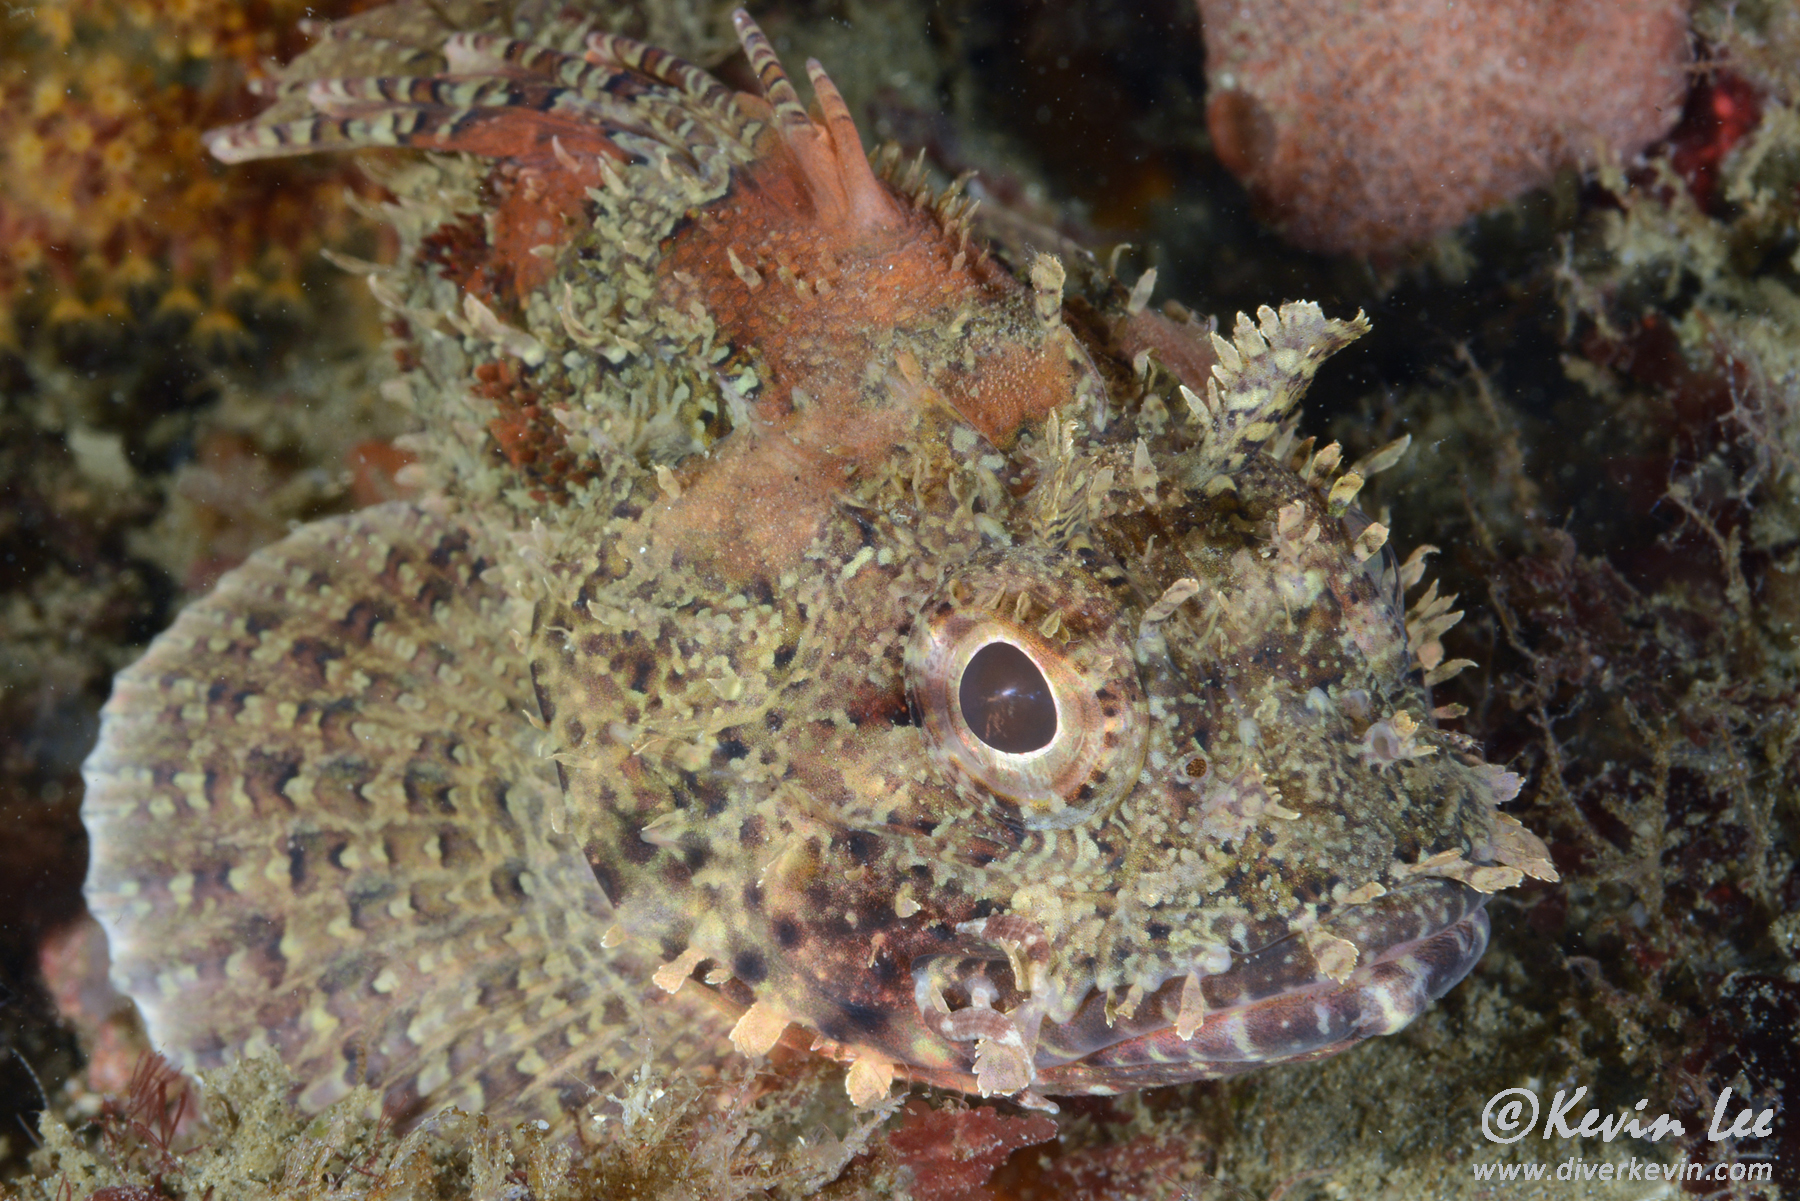
\includegraphics[width=.5\textwidth]{cover_photo}

\end{frame}

\begin{frame}{Early Life History}

\begin{itemize} 
\item[$\bullet$] Migration to spawning grounds, exhibit explosive breeding behavior just before dawn
\item[$\bullet$] External fertilization, females produce hollow gelatenous single-layer floating egg matrix
\item[$\bullet$] Eggs hatch after about 5 days
\item[$\bullet$] Juveniles settle at less than 2 cm 
\end{itemize}

\centering
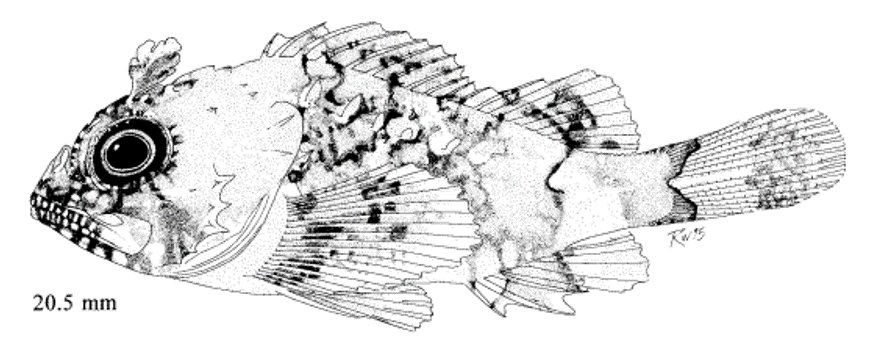
\includegraphics[width=.5\textwidth]{Figures/baby_scorp}

\footnotetext{Line drawning from CalCOFI Atlas 33, pg. 789 Figure 26}

\end{frame}

\begin{frame}{Distribution}

\begin{itemize} 
 \item[$\bullet$] Distributed from central California to Punta Eugenia, Baja California Sur, Mexico 
 \item[$\bullet$] Rarely observed north of Pt. Conception  
 \item[$\bullet$] Observed from the intertidal to 600 ft,  prefer depths of 20-450 ft  
 \item[$\bullet$] Proportion of the stock in Mexican waters unknown
\end{itemize}

\end{frame}

\begin{frame}{Distribution and Stock Assessment Boundary}

\begincols
 \begincol{.5\textwidth} 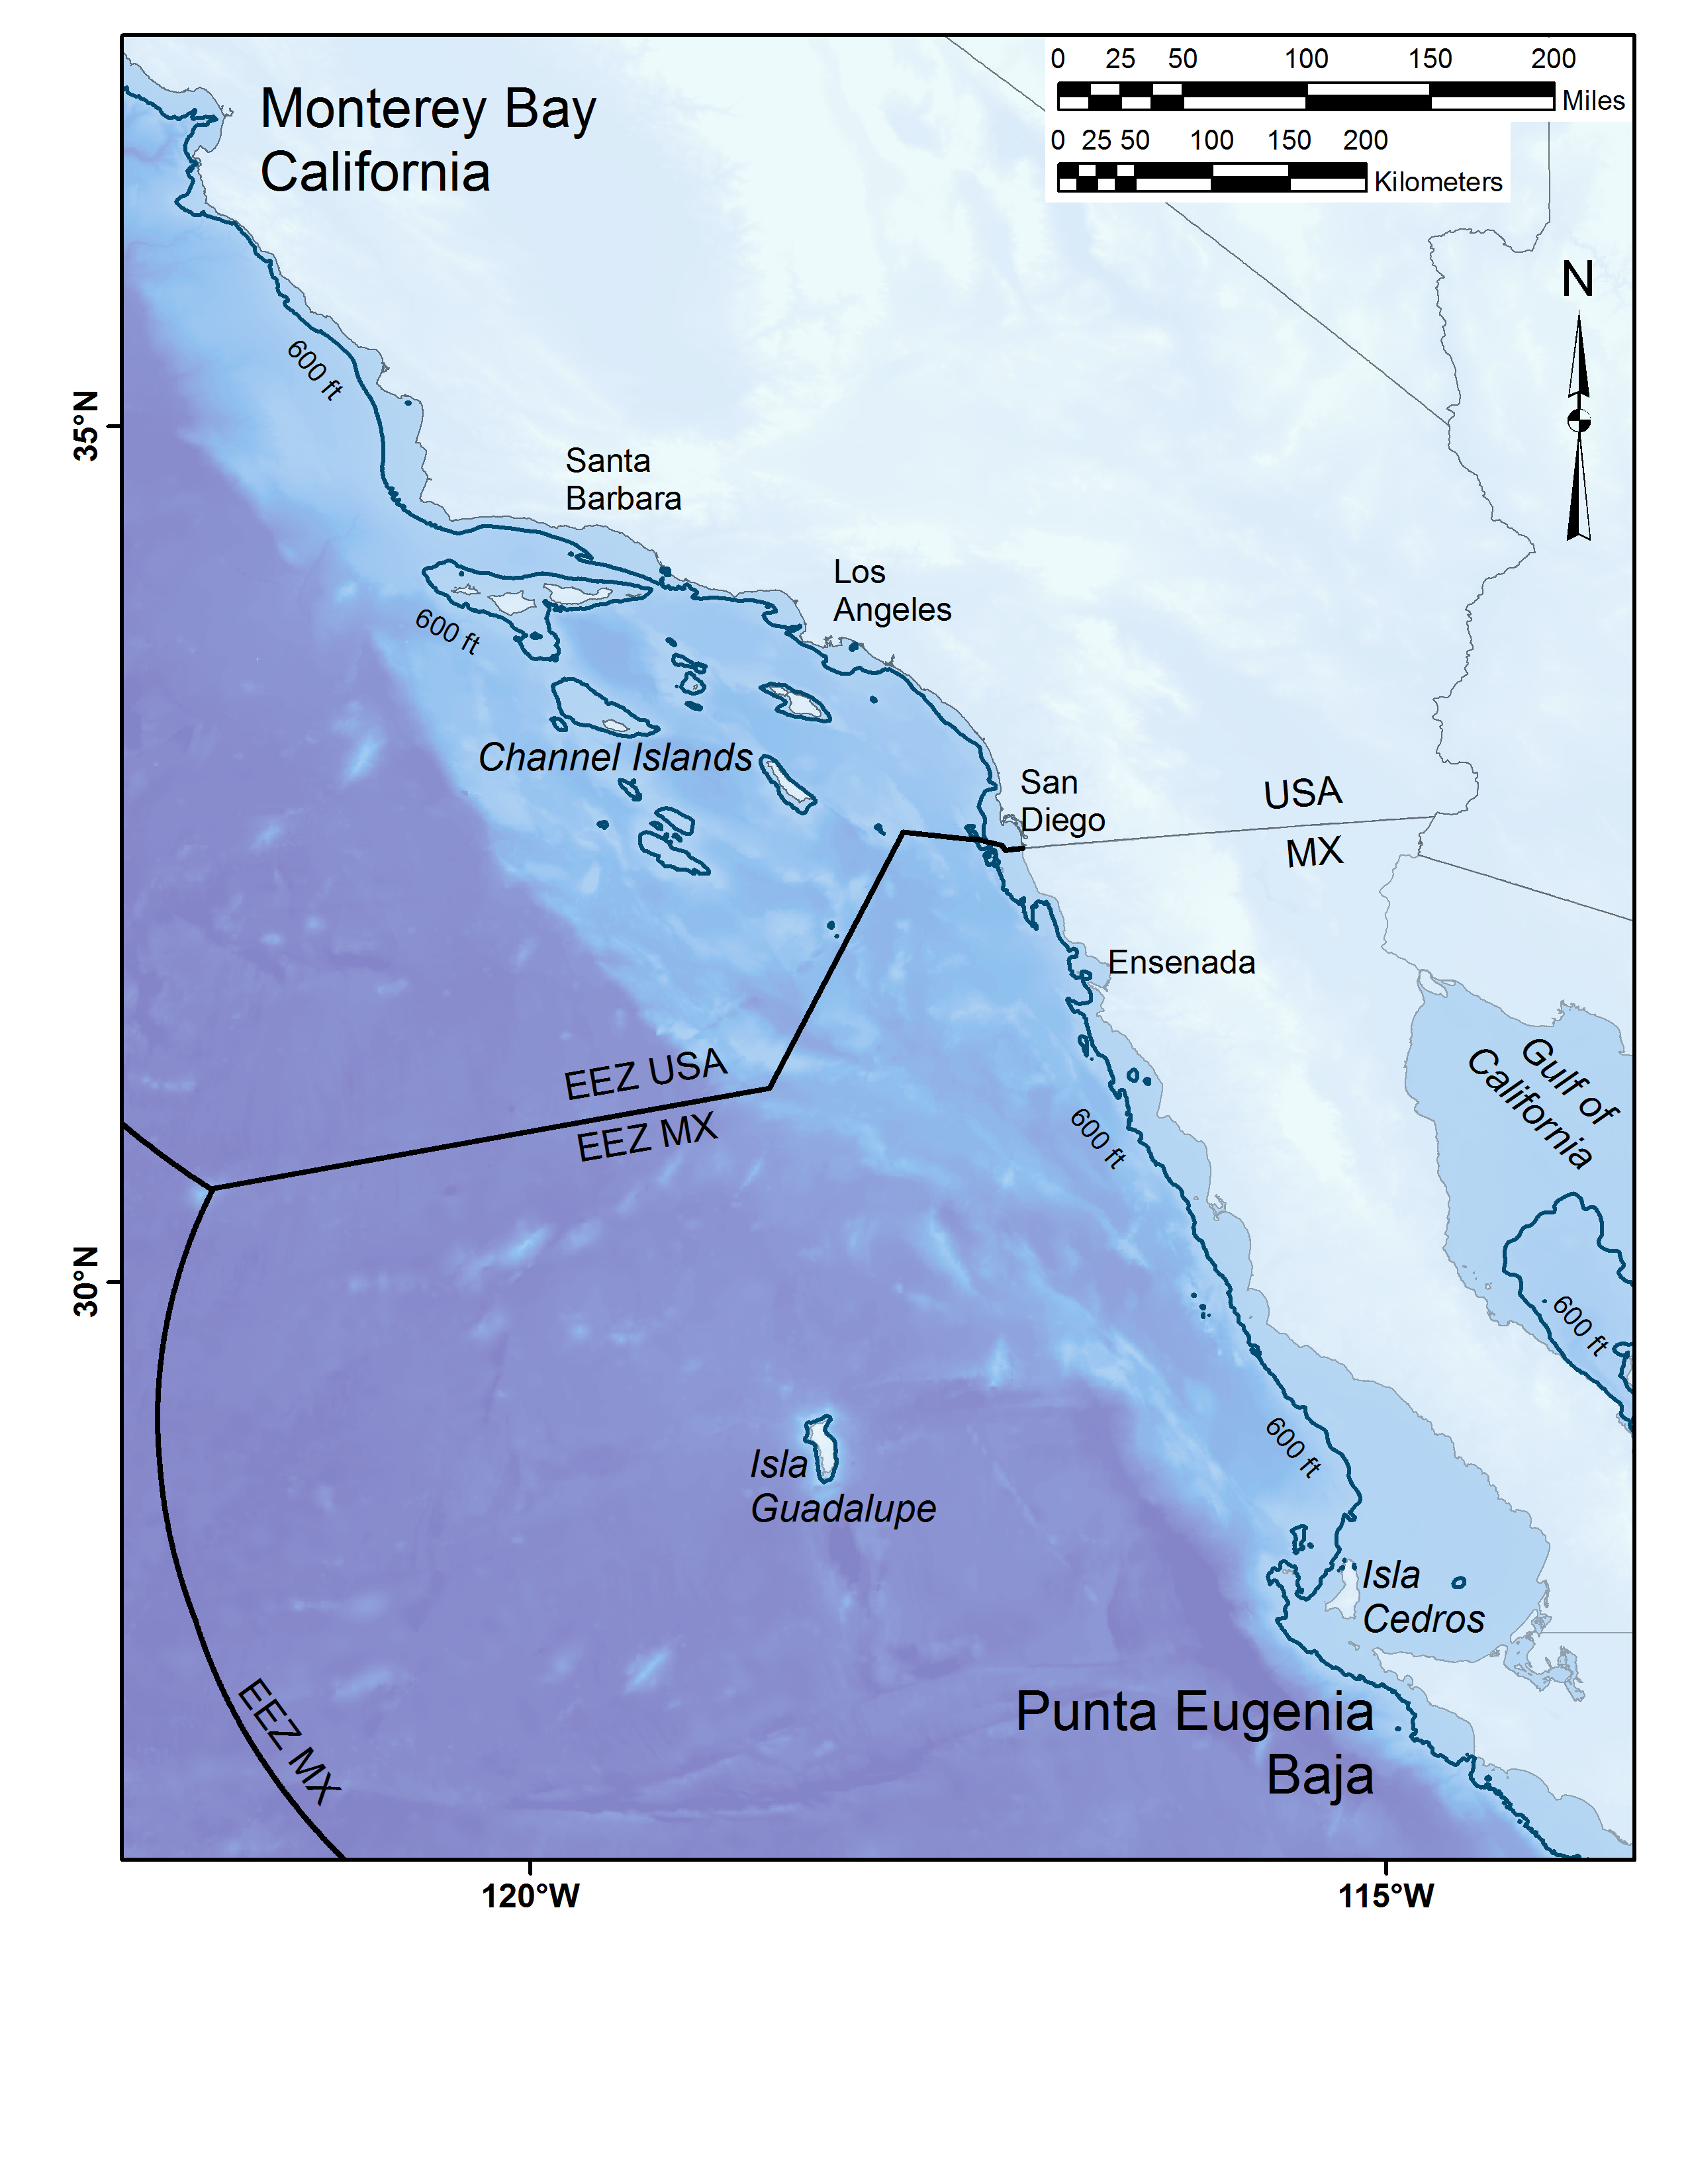
\includegraphics{Figures/Distribution_map.png}

\endcol
 \begincol{.5\textwidth} 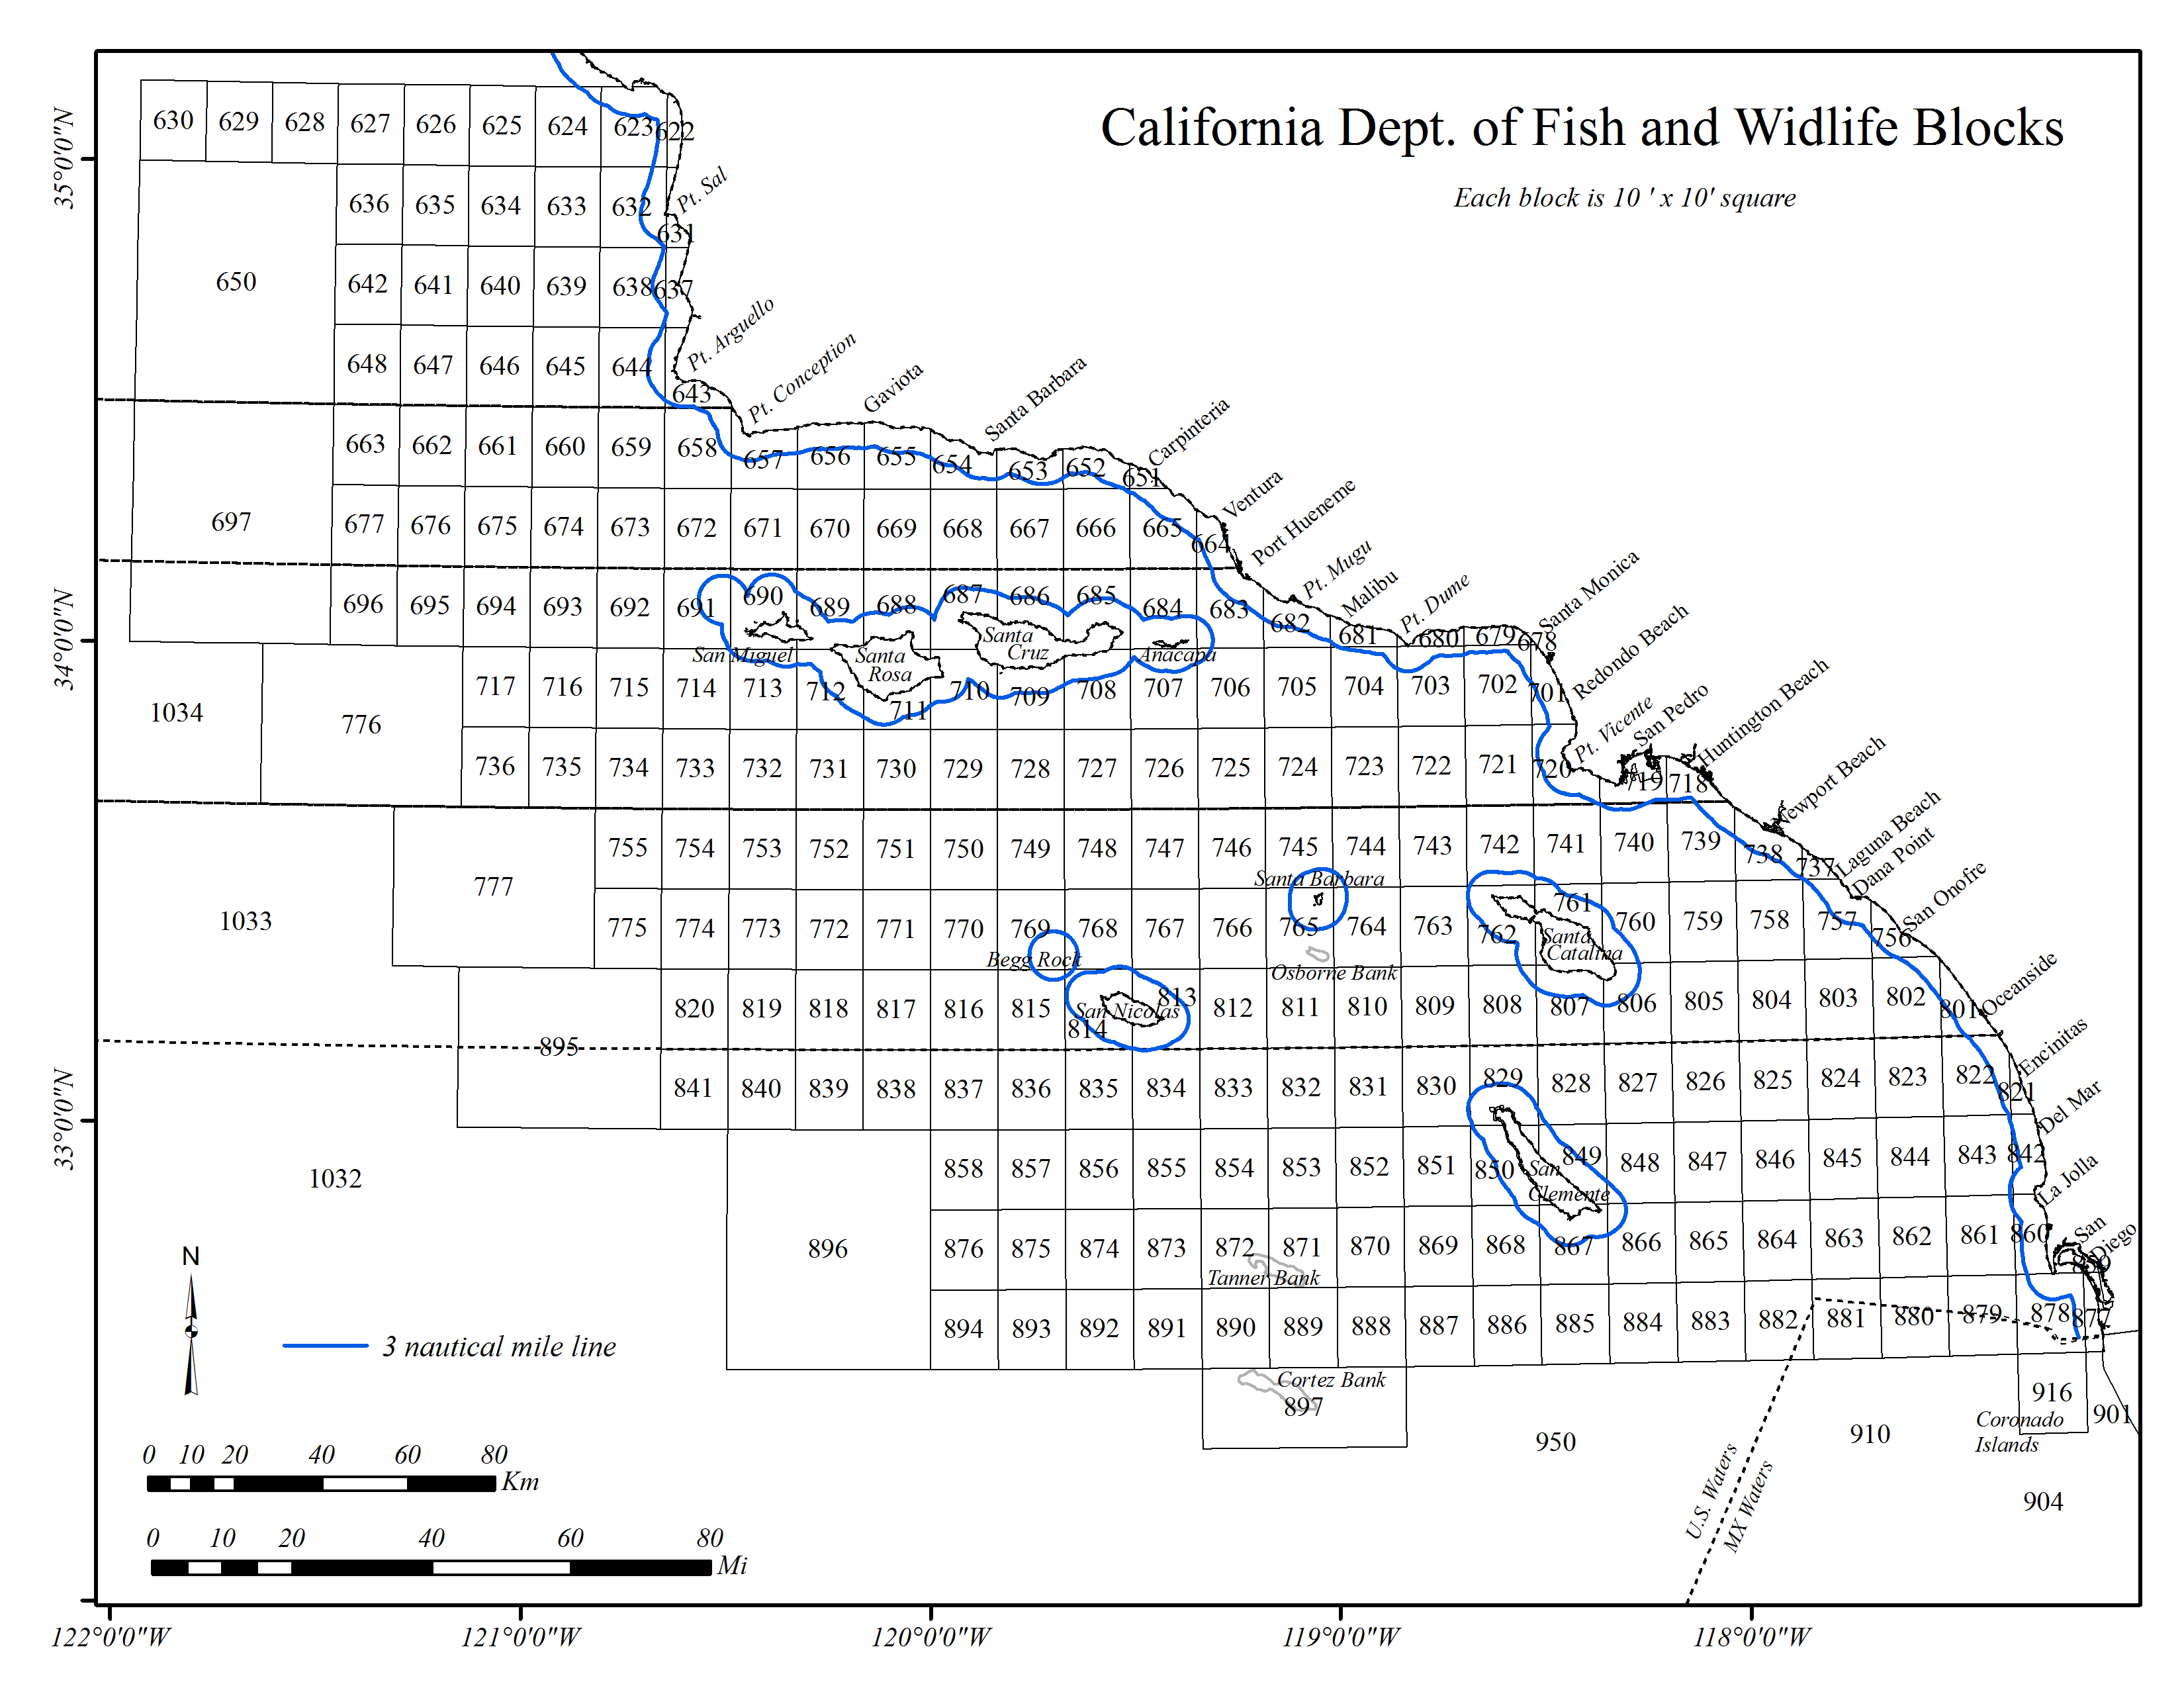
\includegraphics{Figures/assess_region_map.png}
\endcol
\endcols

\end{frame}

\begin{frame}{2005 Stock Assessment}

\begin{itemize}
\item[$\bullet$] Stock first assessed in 2005
\item[$\bullet$] South of Pt. Conception
\item[$\bullet$] $M$ fixed at 0.25
\item[$\bullet$] $h$ fixed at 0.7
\item[$\bullet$] Publicly Owned Treatment Works (POTW) monitoring trawl survey was the axis of uncertainty in the 2005 assessment
\begin{itemize}
\item[$\circ$] POTW survey referred to as the Sanitation District Index in 2005
\end{itemize}
\end{itemize}

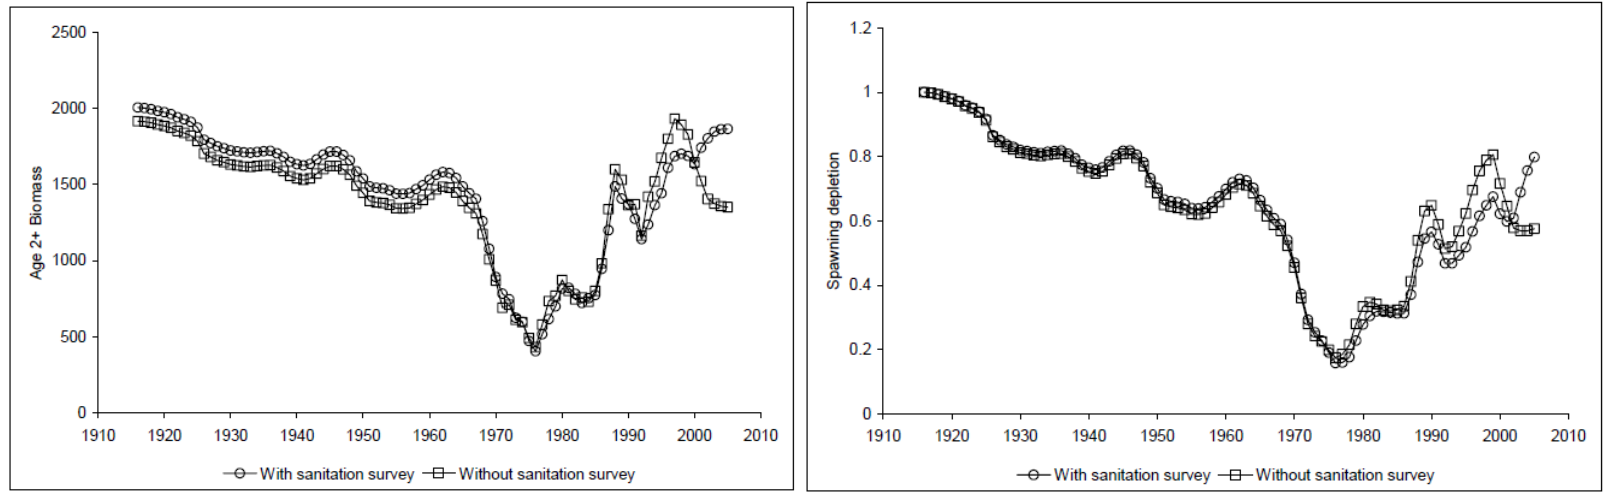
\includegraphics{Figures/2005_bio_depl.png}

\end{frame}

\begin{frame}{2005 Stock Assessment}

\begin{itemize}
\item[$\bullet$] Transitioning from the 2005 assessment, an error was found
\item[$\bullet$] Harvest rate hit the bounds for the recreational fleet
\item[$\bullet$] Not all of the recreational catch was removed in the model
\item[$\bullet$] Input vs. estimated catch was not standard output in SS v.1.8
\end{itemize}

\begincols
 \begincol{.5\textwidth}

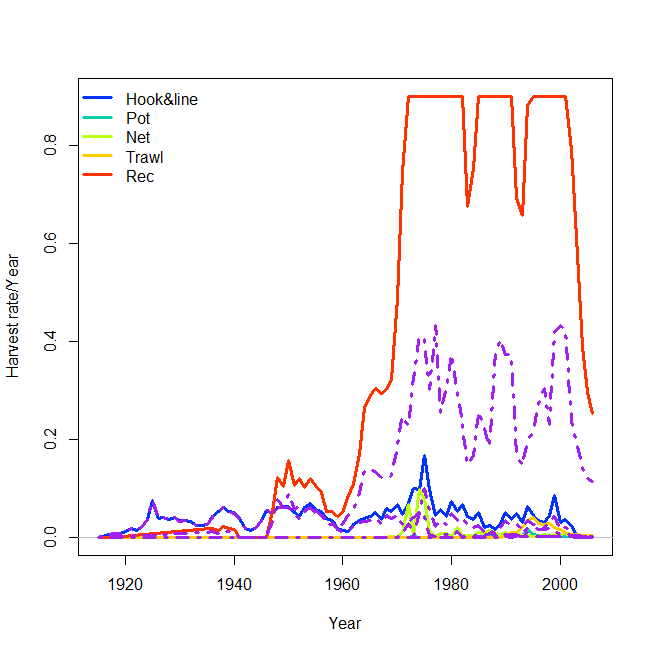
\includegraphics{Figures/bridge_harvestrate.png}

\endcol
 \begincol{.5\textwidth}

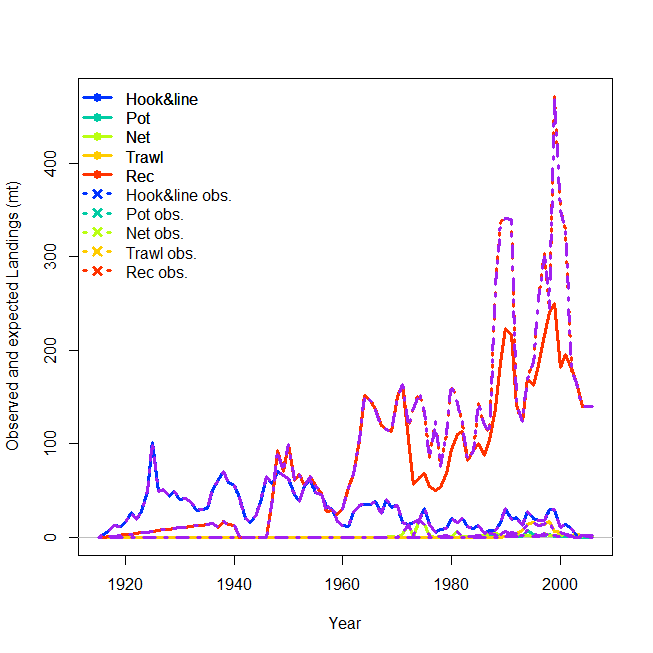
\includegraphics{Figures/bridge_catch.png}

\endcol
\endcols

\end{frame}

\begin{frame}{2005 Stock Assessment}

\begincols
 \begincol{.5\textwidth}

\begin{itemize}
\item[$\bullet$] \textcolor{blue}{2005 assessment, SS v.1.8}
\item[$\bullet$] \textcolor{red}{2005 model in SS3.24z}
\item[$\bullet$] \textcolor{violet}{2017 pre-STAR base model, SS3.30.0.05}
\item[$\bullet$] The two assessments have very similar trends over time, with $B_0$ higher for the 2017 assessment that includes all removals
\end{itemize}

\endcol
 \begincol{.5\textwidth}

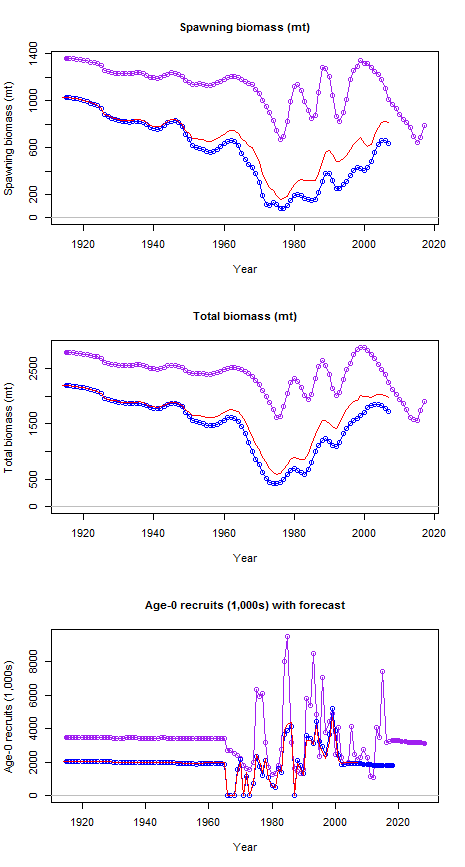
\includegraphics{Figures/bridge_timeseries.png}

\endcol
\endcols

\end{frame}

\begin{frame}{2017 Stock Assessment}

Pre-STAR Base Model

\begin{itemize}
\item[$\bullet$] One area south of Pt. Conception 
\begin{itemize}
\item[$\circ$] Catches from Mexican waters excluded as in 2005
\end{itemize}
\item[$\bullet$] Steepness fixed at 0.718
\item[$\bullet$] Sex-specific $M$ fixed for females, male $M$ estimated as offset
\item[$\bullet$] Re-evaluated fleet definitions
\item[$\bullet$] Ages now available from the NWFSC trawl survey
\item[$\bullet$] New indices and length compositions available
\item[$\bullet$] Newest version of SS allows specification of the minimmum sample size
\end{itemize}

\end{frame}

\section{Catch}\label{catch}

\begin{frame}{Catches by Fleet}

\centering
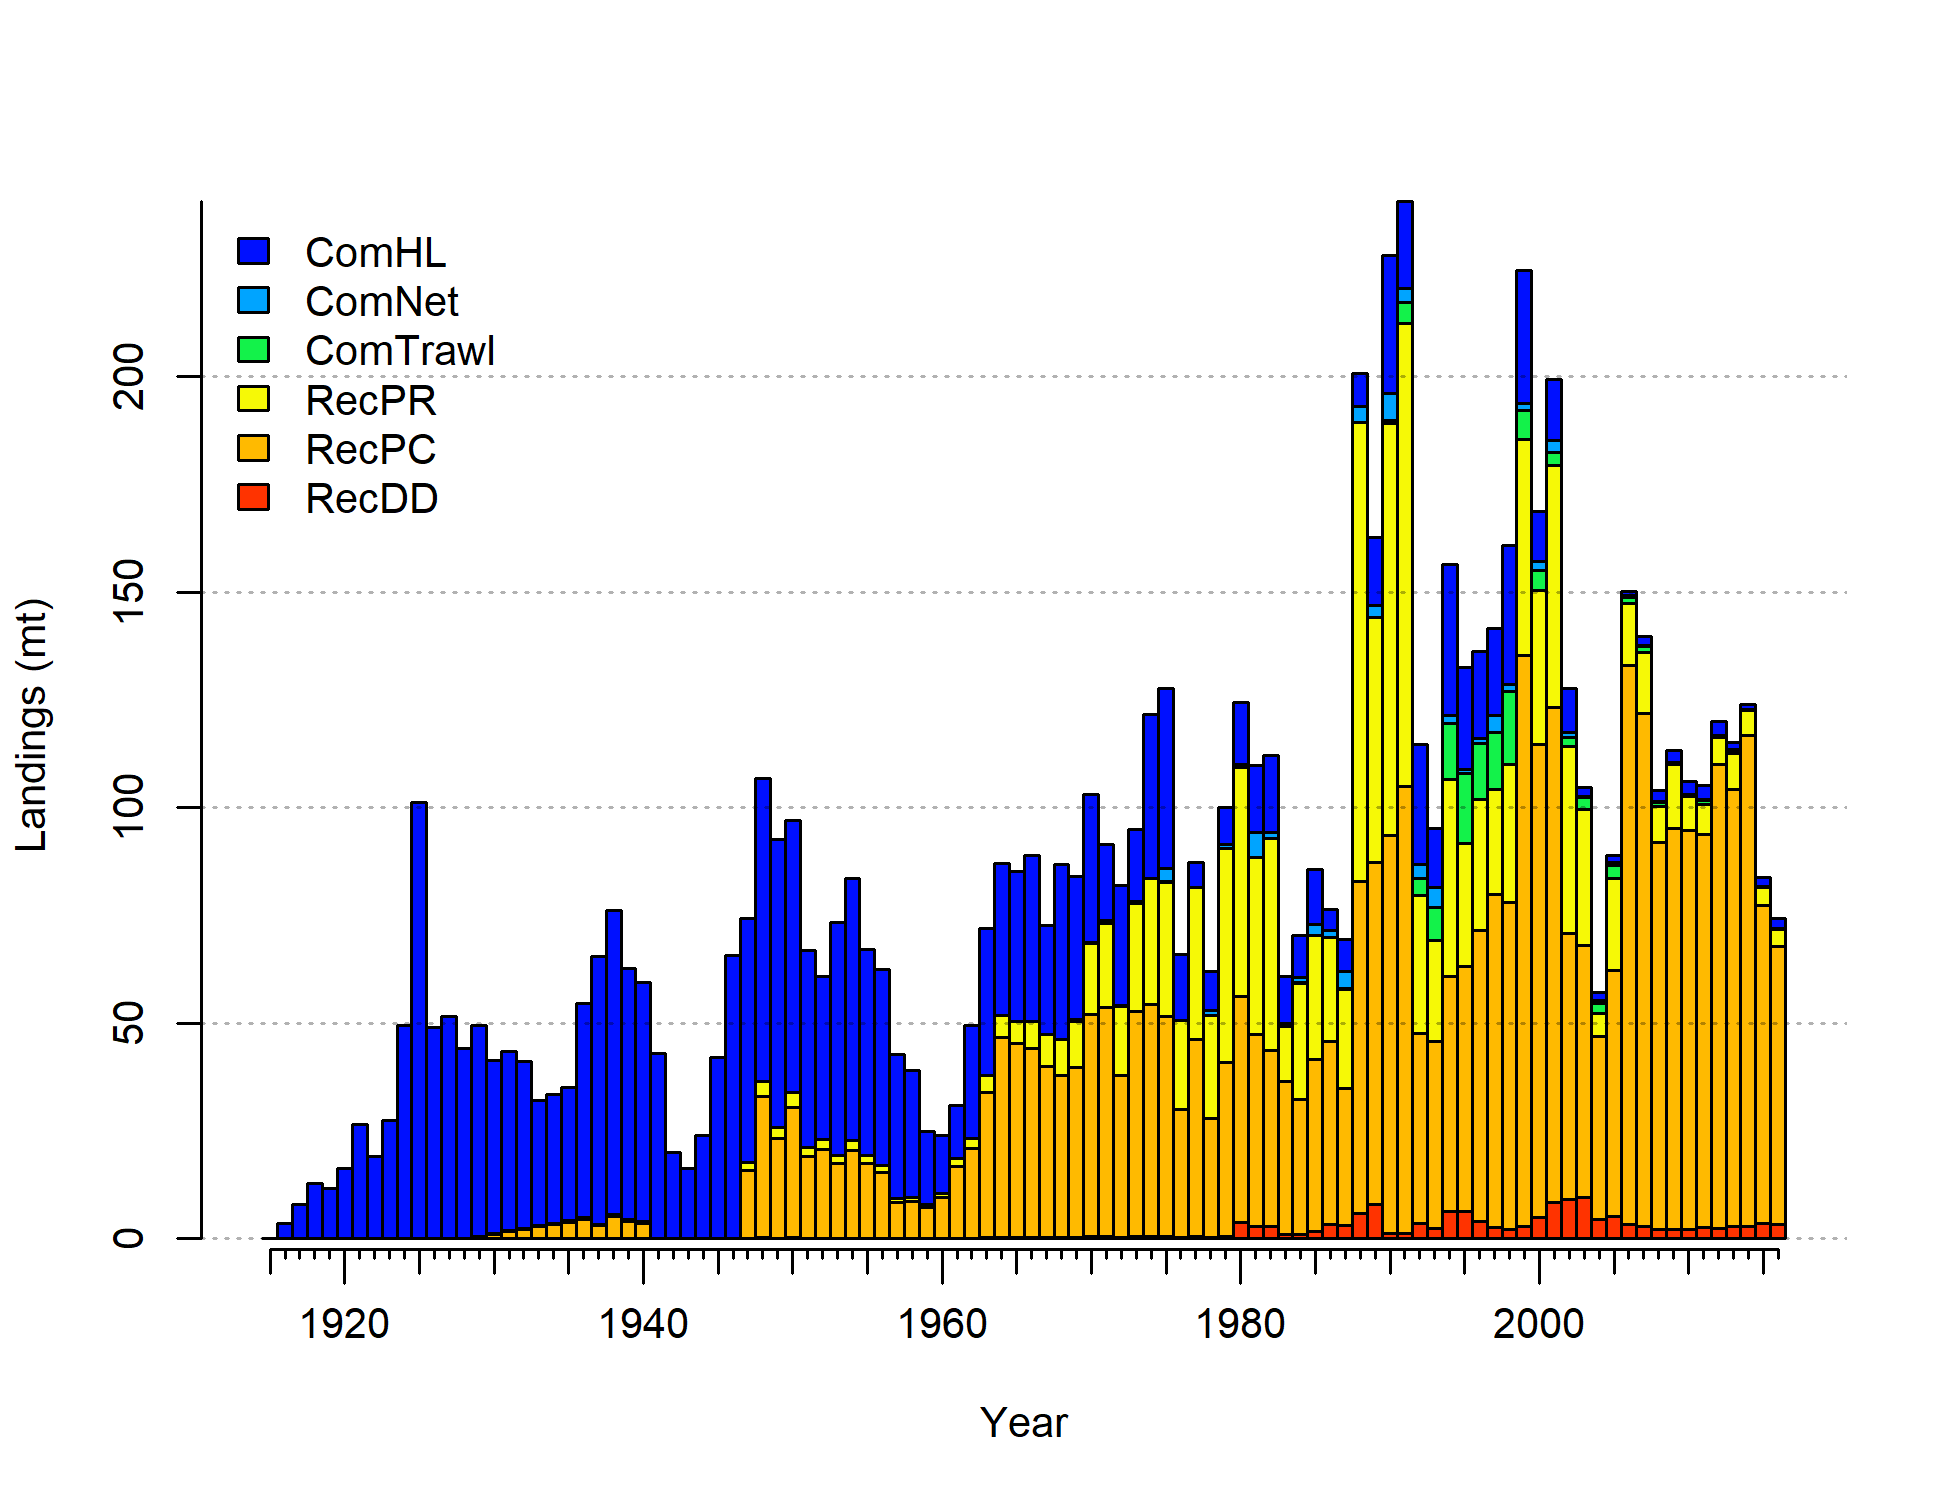
\includegraphics{r4ss/plots_mod1/catch2 landings stacked.png}

\end{frame}

\begin{frame}{Regulations}

\textbf{Recreational}

\begin{itemize}
  \item[\textbf{2000}] 10-in min. size limit, 3 hooks and 1 line   
  \item[\textbf{2001}] 2 hooks and 1 line, Cowcod conservation area  
  \item[\textbf{2002}] Various season length restrictions  
  \item[\textbf{2003}] 20-30 fm depth restriction in 2003, otherwise post-2001 unrestricted or 50 or 60 fm, 5 fish bag limit  
  \end{itemize}

\textbf{Commercial}\\

\begin{itemize}
  \item[\textbf{1999}] 10-in min. size limit, Nearshore fishery permit with restricted access at 1100 permits
  \item[\textbf{3003}]  Nearshore fishery permit with restricted access at 200 permits
  \end{itemize}

\end{frame}

\begin{frame}{Regulations - depth and closures}

Commercial (left) and Recreational (right) \begincols
 \begincol{.4\textwidth} 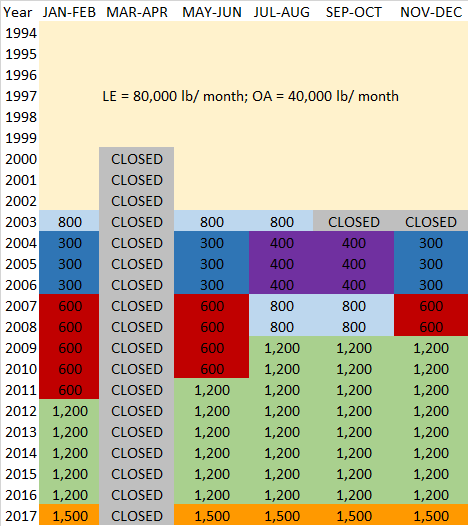
\includegraphics{Figures/Com_regs.png} \endcol
 \begincol{.6\textwidth} 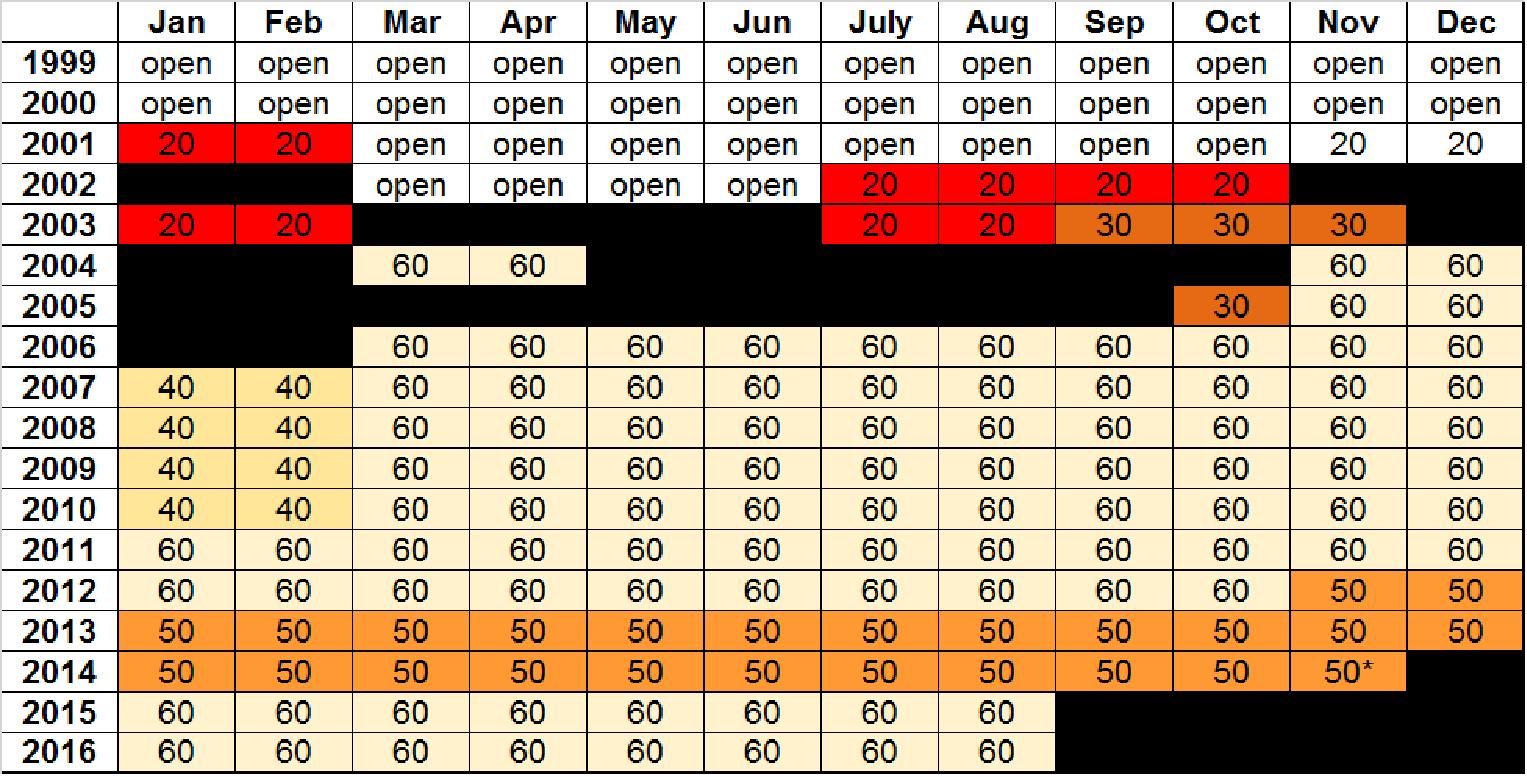
\includegraphics{Figures/Rec_regs.pdf}\\
\endcol
\endcols

\end{frame}

\begin{frame}{U.S. and Mexico Catch}

\includegraphics{California_scorpionfish_2017_files/figure-latex/unnamed-chunk-18-1.pdf}

\end{frame}

\begin{frame}{Recreational Catch}

\begincols
 \begincol{.4\textwidth}

\begin{itemize}
\item[$\bullet$] 2005 assessment used number of fish for recreational catches
\item[$\bullet$] 2017 assessment includes one recreational discard fleet
\begin{itemize}
\item[$\circ$] Discard mortality rate of 7\%
\item[$\circ$] Discard biomass accounts for  $<$3\% of recreational mortality
\end{itemize}
\end{itemize}

\endcol
 \begincol{.6\textwidth}
\includegraphics[totalheight=0.65\textheight]{California_scorpionfish_2017_files/figure-latex/unnamed-chunk-16-1.pdf}\\
\endcol
\endcols

\end{frame}

\begin{frame}{Commercial Catch}

\begincols
 \begincol{.4\textwidth}

\begin{itemize}
  \item[$\bullet$] Historical catches same as the 2005 assessment
  \item[$\bullet$] California Fisheries Information System (CFIS) landings data used to update catches from 2005-2016 
  \item[$\bullet$] Discards assumed neglible
\end{itemize}

\endcol
 \begincol{.55\textwidth}
\includegraphics{California_scorpionfish_2017_files/figure-latex/unnamed-chunk-17-1.pdf}
\endcol
\endcols

\end{frame}

\section{Indices}\label{indices}

\begin{frame}{Indices of Abundance}

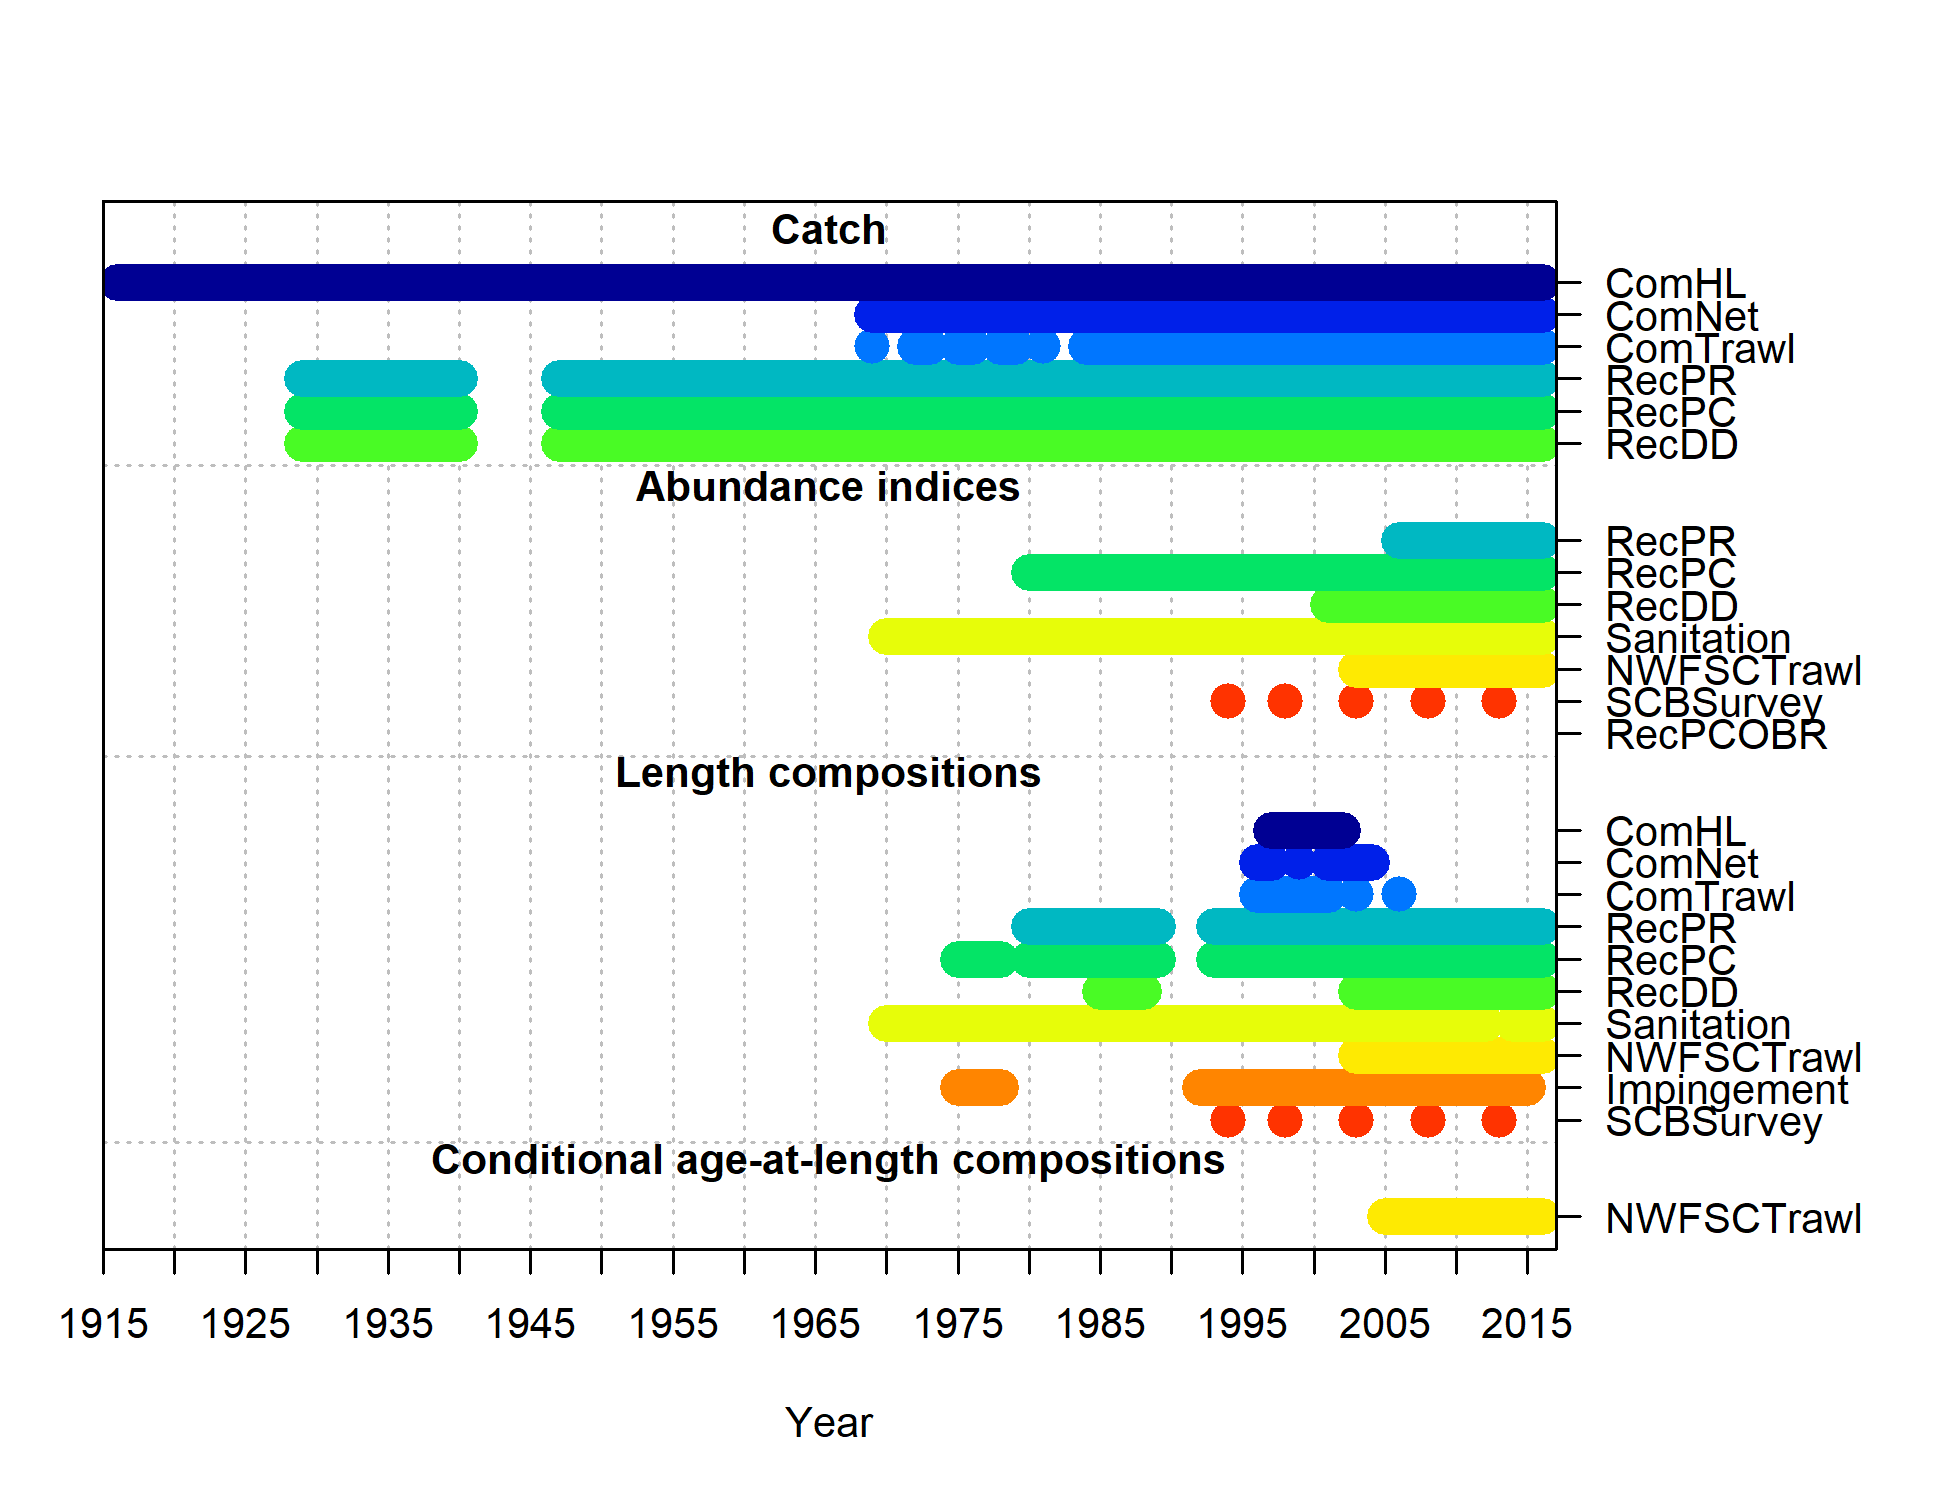
\includegraphics{r4ss/plots_mod1/data_plot.png}

\end{frame}

\begin{frame}{Indices of Abundance}

\begin{itemize}
\tightlist
\item
  All of the methods used to standardize indices have been endorsed by
  the SSC
\end{itemize}

\begin{table}[ht]
\centering
\scalebox{0.7}{
\begin{tabular}{p{2.5in}p{0.8in}p{.4in}p{2in}}
  \hline
Name & Years & Fishery ind. & Method \\ 
  \hline
Recreational PR dockside CPUE & 2004-2016 & No & delta-GLM (bin-lognormal) \\ 
  CPFV logbook CPUE & 1980-2016 & No & negative binomial \\ 
  Onboard observer discard catch CPUE & 2002-2016 & No & delta-GLM (bin-lognormal) \\ 
  Sanitation district CPUE & 1970-2016 & Yes & delta-GLM (bin-lognormal) \\ 
  NWFSC trawl survey CPUE & 2003-2016 & Yes & VAST \\ 
  CSUN/VRG Gillnet survey CPUE & 1995-2008 & Yes & delta-GLM (bin-lognormal) \\ 
  Southern California Bight trawl survey CPUE & '94, '98, '03, '08, '13 & Yes & delta-GLM (bin-lognormal) \\ 
  Onboard observer retained catch CPUE & 2002-2016 & No & delta-GLM (bin-lognormal) \\ 
   \hline
\end{tabular}
}
\end{table}

\end{frame}

\begin{frame}{Indices of Abundance}

\textbf{Delta-GLM Approach}

\begin{itemize}
\item[$\bullet$] Approach used for all indices excpet the NWFSC trawl survey and the CPFV logbook 
\item[$\bullet$] Two-part model
\begin{itemize}
\item[$\circ$] Binomial for to the presence-absence data
\item[$\circ$] Lognormal of Gamma fit to positives
\end{itemize}
\item[$\bullet$] General approach 
\begin{itemize}
\item[$\circ$] Filter data to identify most appropriate samples 
\item[$\circ$] Model selection
\begin{itemize}
\item[$\cdot$] Gamma or Lognormal for positives
\item[$\cdot$] Covariates for each of the two models chosen using AIC
\end{itemize}
\end{itemize}
\item[$\circ$] Uncertainty for final model estimated via jackknifing 
\end{itemize}

\end{frame}

\begin{frame}{Recreational Dockside Private Boat Index}

\textbf{Sample}: California CRFS only; \textbf{Years}: 2006-2016;
\textbf{Effort}: Angler days

\begincols
 \begincol{.6\textwidth}

\begin{table}[ht]
\centering
\scalebox{0.5}{
\begin{tabular}{p{1.4in}p{2in}p{.5in}p{.5in}}
  \hline
Filter & Criteria & Pos. Trips & Trips \\ 
  \hline
Entire dataset &  &  & 108,171 \\ 
  General data filters & CRFS-PR1 survey only, Southern California only (sub\_reg = 1), Hook and line gear only (geara = 'H'), Ocean only (Area\_X = 1 or 2) & 3,802 & 43,956 \\ 
  Region & Remove trips from Santa Barbara & 3,757 & 42,956 \\ 
  Year & Remove 2004-2005; fishery closed majority of year & 3,094 & 33,770 \\ 
  Closed fishery & Remove remaining trips when fishery closed & 3,056 & 32,236 \\ 
  Rare and co-occurring species & Remove trips with yellowfin tuna and dolphinfish and species present in $<$1\% of all trips and in at least 5 years of data & 3,056 & 30,033 \\ 
  Stephens-MacCall & Retain all positive trips, plus "False Positives" (trips predicted to be in California scorpionfish habitat, but with no California scorpionfish retained) & 3,056 & \textbf{8,590} \\ 
   \hline
\end{tabular}
}
\end{table}

\endcol
 \begincol{.4\textwidth}

\begin{table}[ht]
\centering
\scalebox{0.55}{
\begin{tabular}{p{1.8in}p{.5in}p{.5in}}
  \hline
Model & Binomial & Lognormal \\ 
  \hline
~Year & 6182 & 8103 \\ 
  ~Year + County & 5862 & 8003 \\ 
  ~Year + Wave & 6091 & 8092 \\ 
  ~Year + County + Wave & \textbf{5792} & \textbf{8000} \\ 
   \hline
\end{tabular}
}
\end{table}

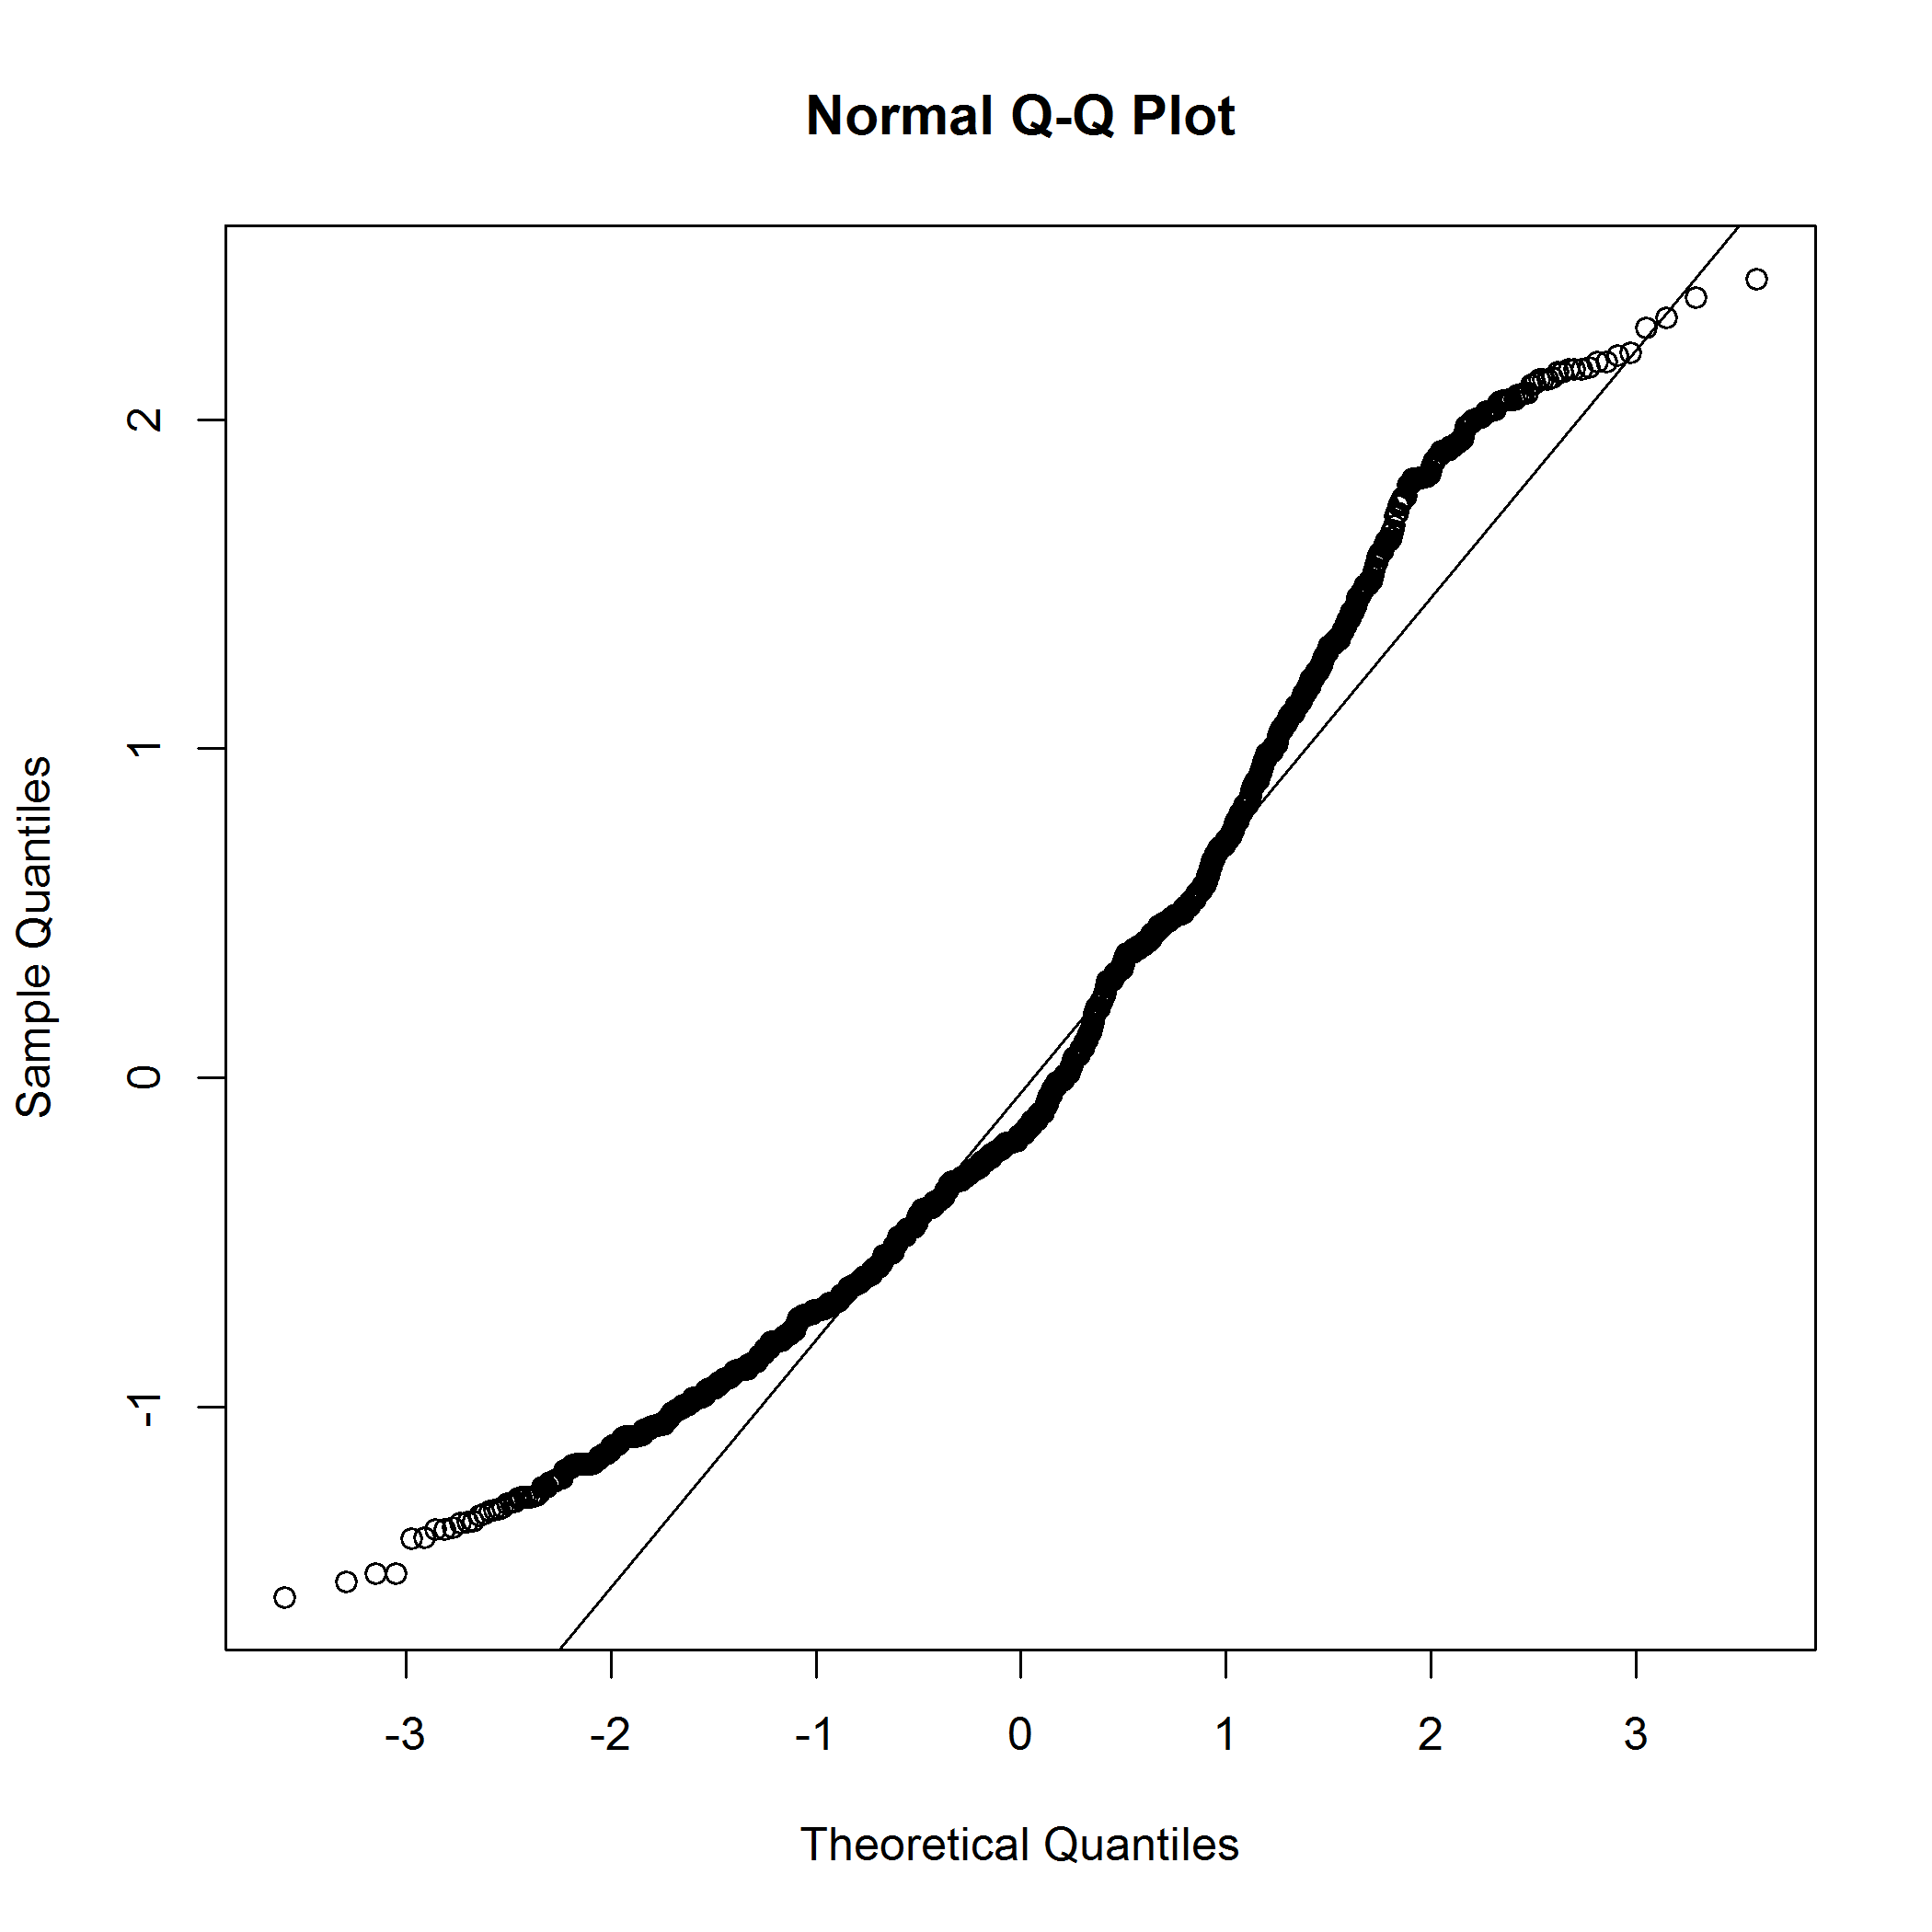
\includegraphics[height=5cm]{Figures/Fleet4_RecPR_dockside_QQ.png}

\endcol
\endcols

\end{frame}

\begin{frame}{Recreational Dockside Private Boat Index}

\begincols
 \begincol{.5\textwidth}

\begin{itemize}
\item[$\bullet$] Positive indicators: treefish, barred sandbass, ocean whitefish, cabezon
\item[$\bullet$] Negative indicators: yellowtail amberjack, bat rays, white croaker, white seabass
\item[$\bullet$] Similar indicator species as in the MRFSS party/charter analysis
\end{itemize}

\endcol
 \begincol{.5\textwidth}

\centering
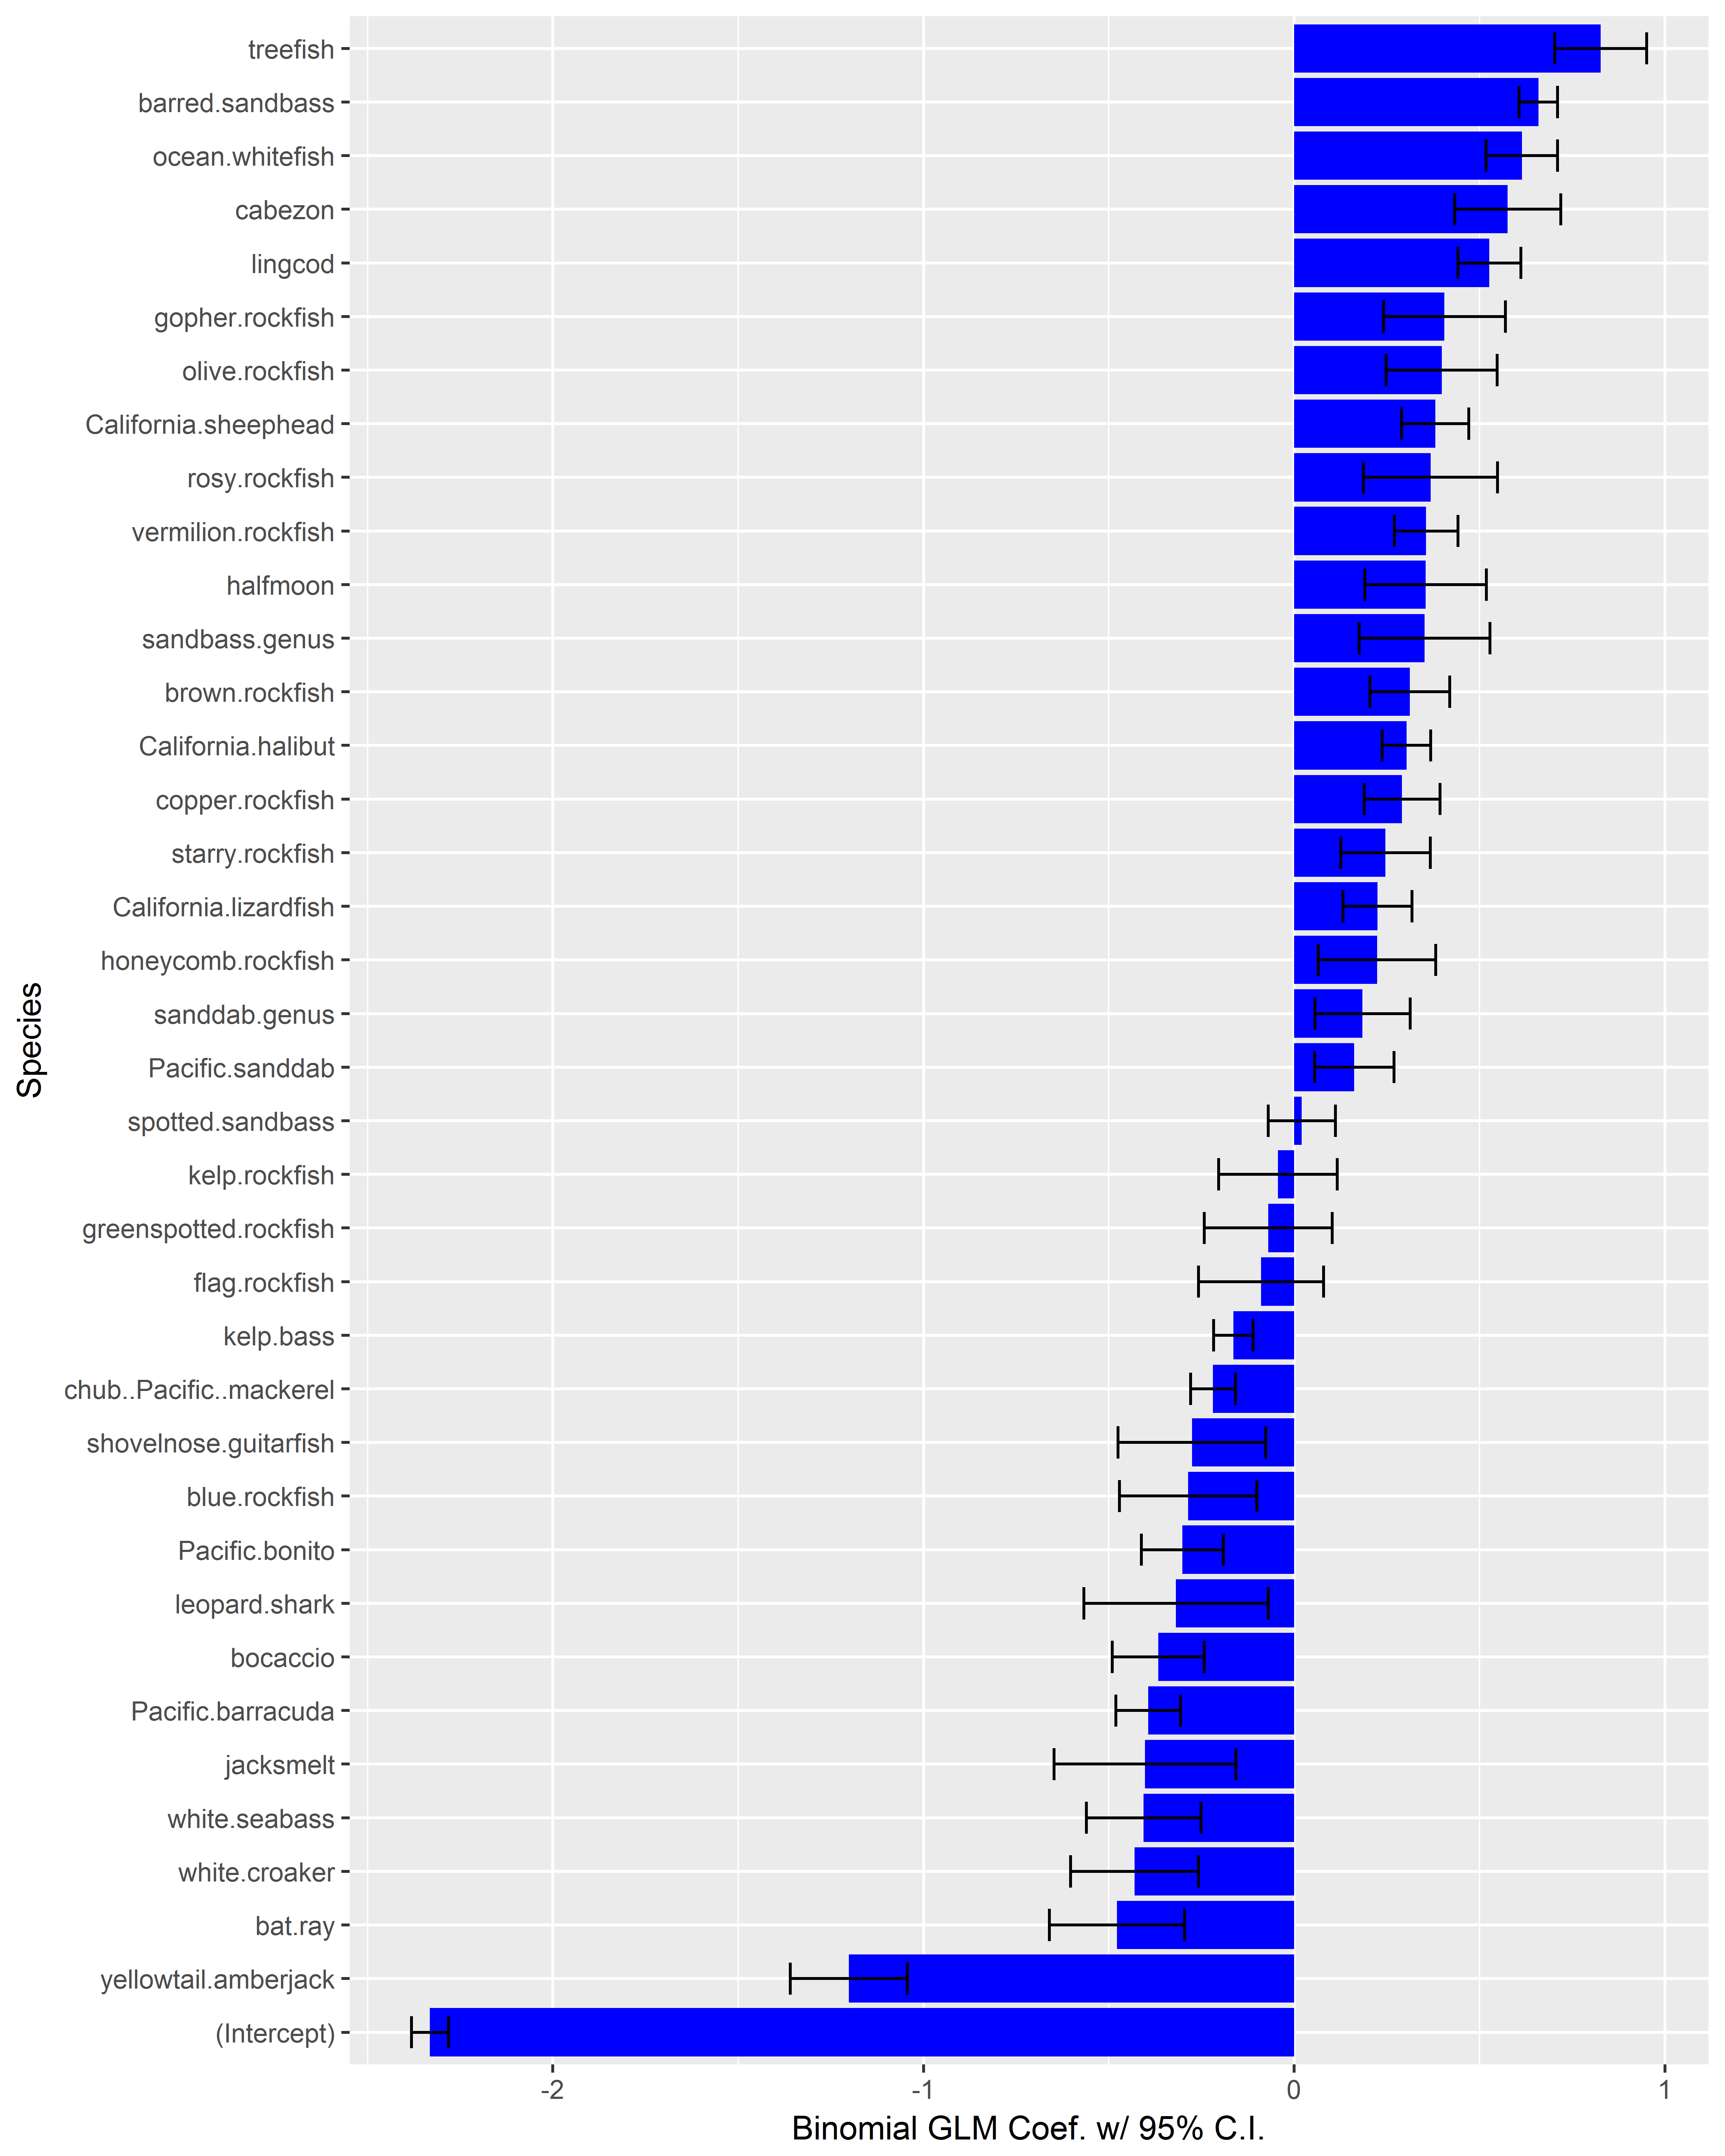
\includegraphics[height=8cm]{Figures/Fleet4_RecPR_SMcoef.png}

\endcol
\endcols

\end{frame}

\begin{frame}{Recreational Dockside Private Boat Index}

\textbf{Results}

\centering
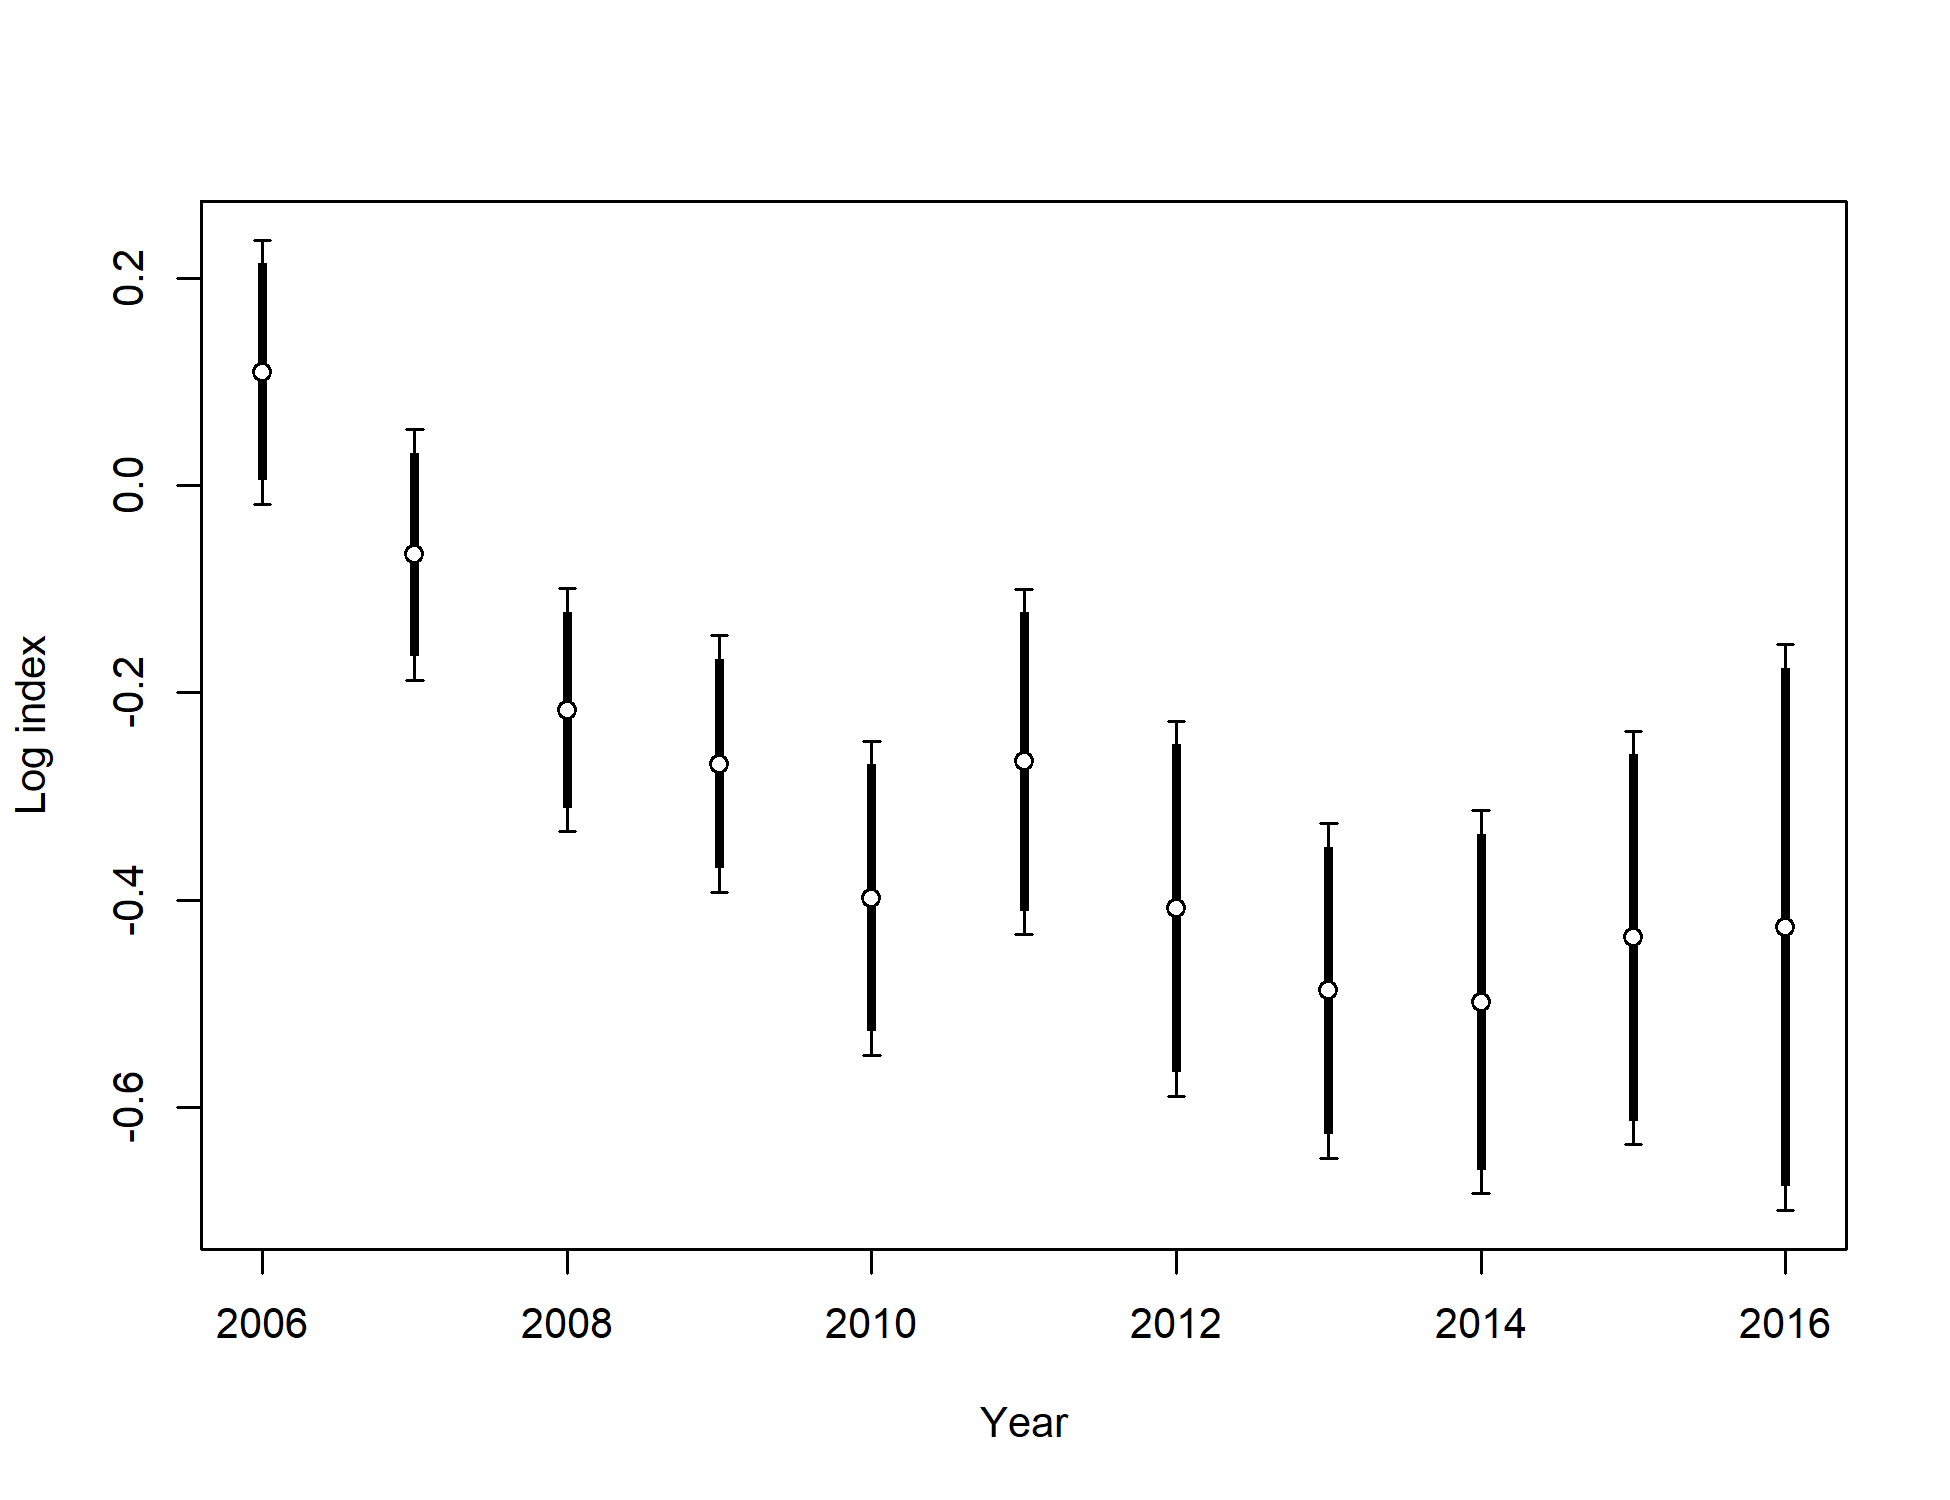
\includegraphics{r4ss/plots_mod1/index4_logcpuedata_RecPR.png}

\end{frame}

\begin{frame}{Recreational CPFV Logbook Index}

\textbf{Sample}: Captain-reported catch; \textbf{Years}: 1980-2016;
\textbf{Effort}: Angler hours

\begin{table}[ht]
\centering
\scalebox{0.5}{
\begin{tabular}{p{2.4in}p{2.6in}p{.6in}}
  \hline
Filter & Criteria & Trips \\ 
  \hline
All CA data & No filter & 1,164,662 \\ 
  Gear & Remove trips reported as diving, mooching or trolling & 959,740 \\ 
  Effort or missing data & Remove trips with missing effort or species information & 930,233 \\ 
  Year & Remove 2017, remaining years 1980-2016 & 929,781 \\ 
  Region & Remove trips north of Pt. Conception and in Mexico & 568,222 \\ 
  Fish encountered & Remove trips reporting number of retained fish greater than in the 99\% quantile ($>$325 fish) & 564,433 \\ 
  Target species & Remove trips targeting sharkes, striped bass, sturgeon, tuna, misc. bay, and potluck & 558,872 \\ 
  Single-species trips & Filter trips reporting catches of only species and that one species in $<$100 trips & 558,833 \\ 
  Offshore trips & Remove trips catching yellowtail, tunas, and dolphinfish that were not designated as offshore trips & 475,492 \\ 
  Vessel & Remove trips by vessels that had fewer than 10 trips catching scorpionfish & 466,023 \\ 
  Anglers & Remove trips with number of anglers $<$ the 1\% and $>$ the 99\% quantile (retain 5-75 anglers) & 452,938 \\ 
  Depth & Remove trips in blocks with a minimum depth of $>$140m & 443,929 \\ 
  Scorpionfish targets & Blocks with at least 100 scorpionfish trips & 433,248 \\ 
  Sample size & Blocks with at least 500 trips & \textbf{432,868} \\ 
   \hline
\end{tabular}
}
\end{table}

\end{frame}

\begin{frame}{Recreational CPFV Logbook Index}

\textbf{Results}

\begincols
 \begincol{.4\textwidth}

\begin{table}[ht]
\centering
\scalebox{0.6}{
\begin{tabular}{p{1.6in}p{1.5in}}
  \hline
Model & Negative Binomial \\ 
  \hline
Year & 1918470 \\ 
  Year+ Month & 1901592 \\ 
  Year + Block & 1872224 \\ 
  Year+ Month + Block & \textbf{1854652} \\ 
   \hline
\end{tabular}
}
\end{table}

\endcol
 \begincol{.6\textwidth}

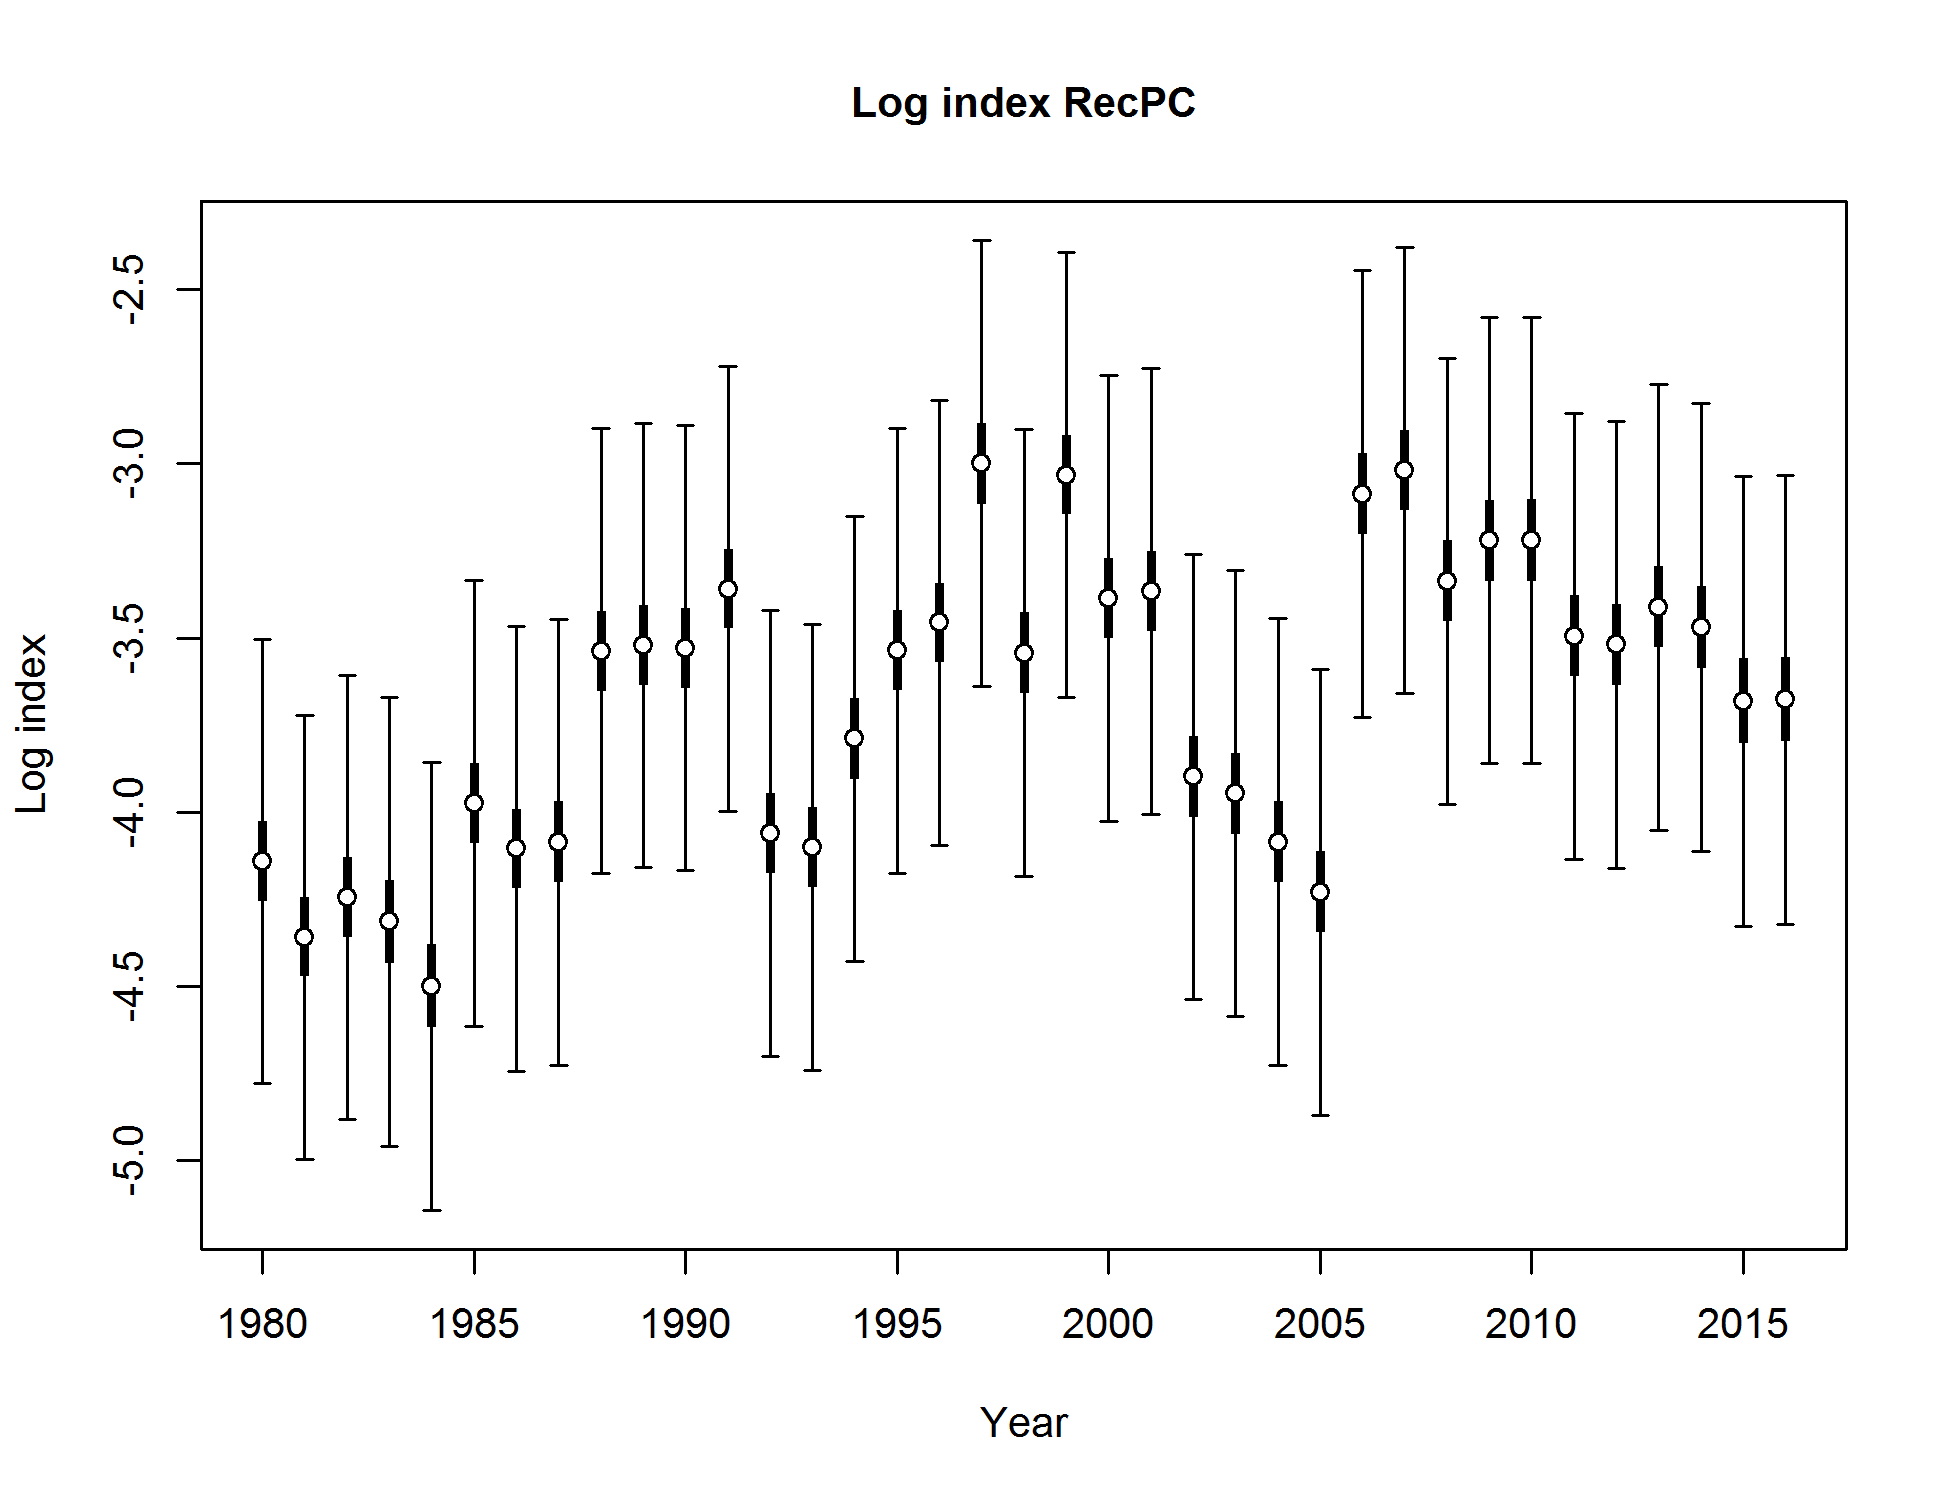
\includegraphics{r4ss/plots_mod1/index4_logcpuedata_RecPC.png} \endcol
\endcols

\end{frame}

\begin{frame}{Recreational Dockside Party/Charer Boat Index}

\textbf{Sample}: California MRFSS ; \textbf{Years}: 1980-2003;
\textbf{Effort}: Angler hours

\begincols
 \begincol{.5\textwidth}

\begin{itemize}
\item[$\bullet$] \emph{Index not used in the assessment}
\item[$\bullet$] No MRFSS sampling from 1990-1992
\item[$\bullet$] Index sensitive to Stephens-MacCall threshold
\item[$\bullet$] Dockside index estimate for 1989 is high and anomolous
\item[$\bullet$] Data redundant with the CPFV logbook index
\item[$\bullet$] 1989 estimate lower if a higher threshold is used
\end{itemize}

\endcol
 \begincol{.5\textwidth}

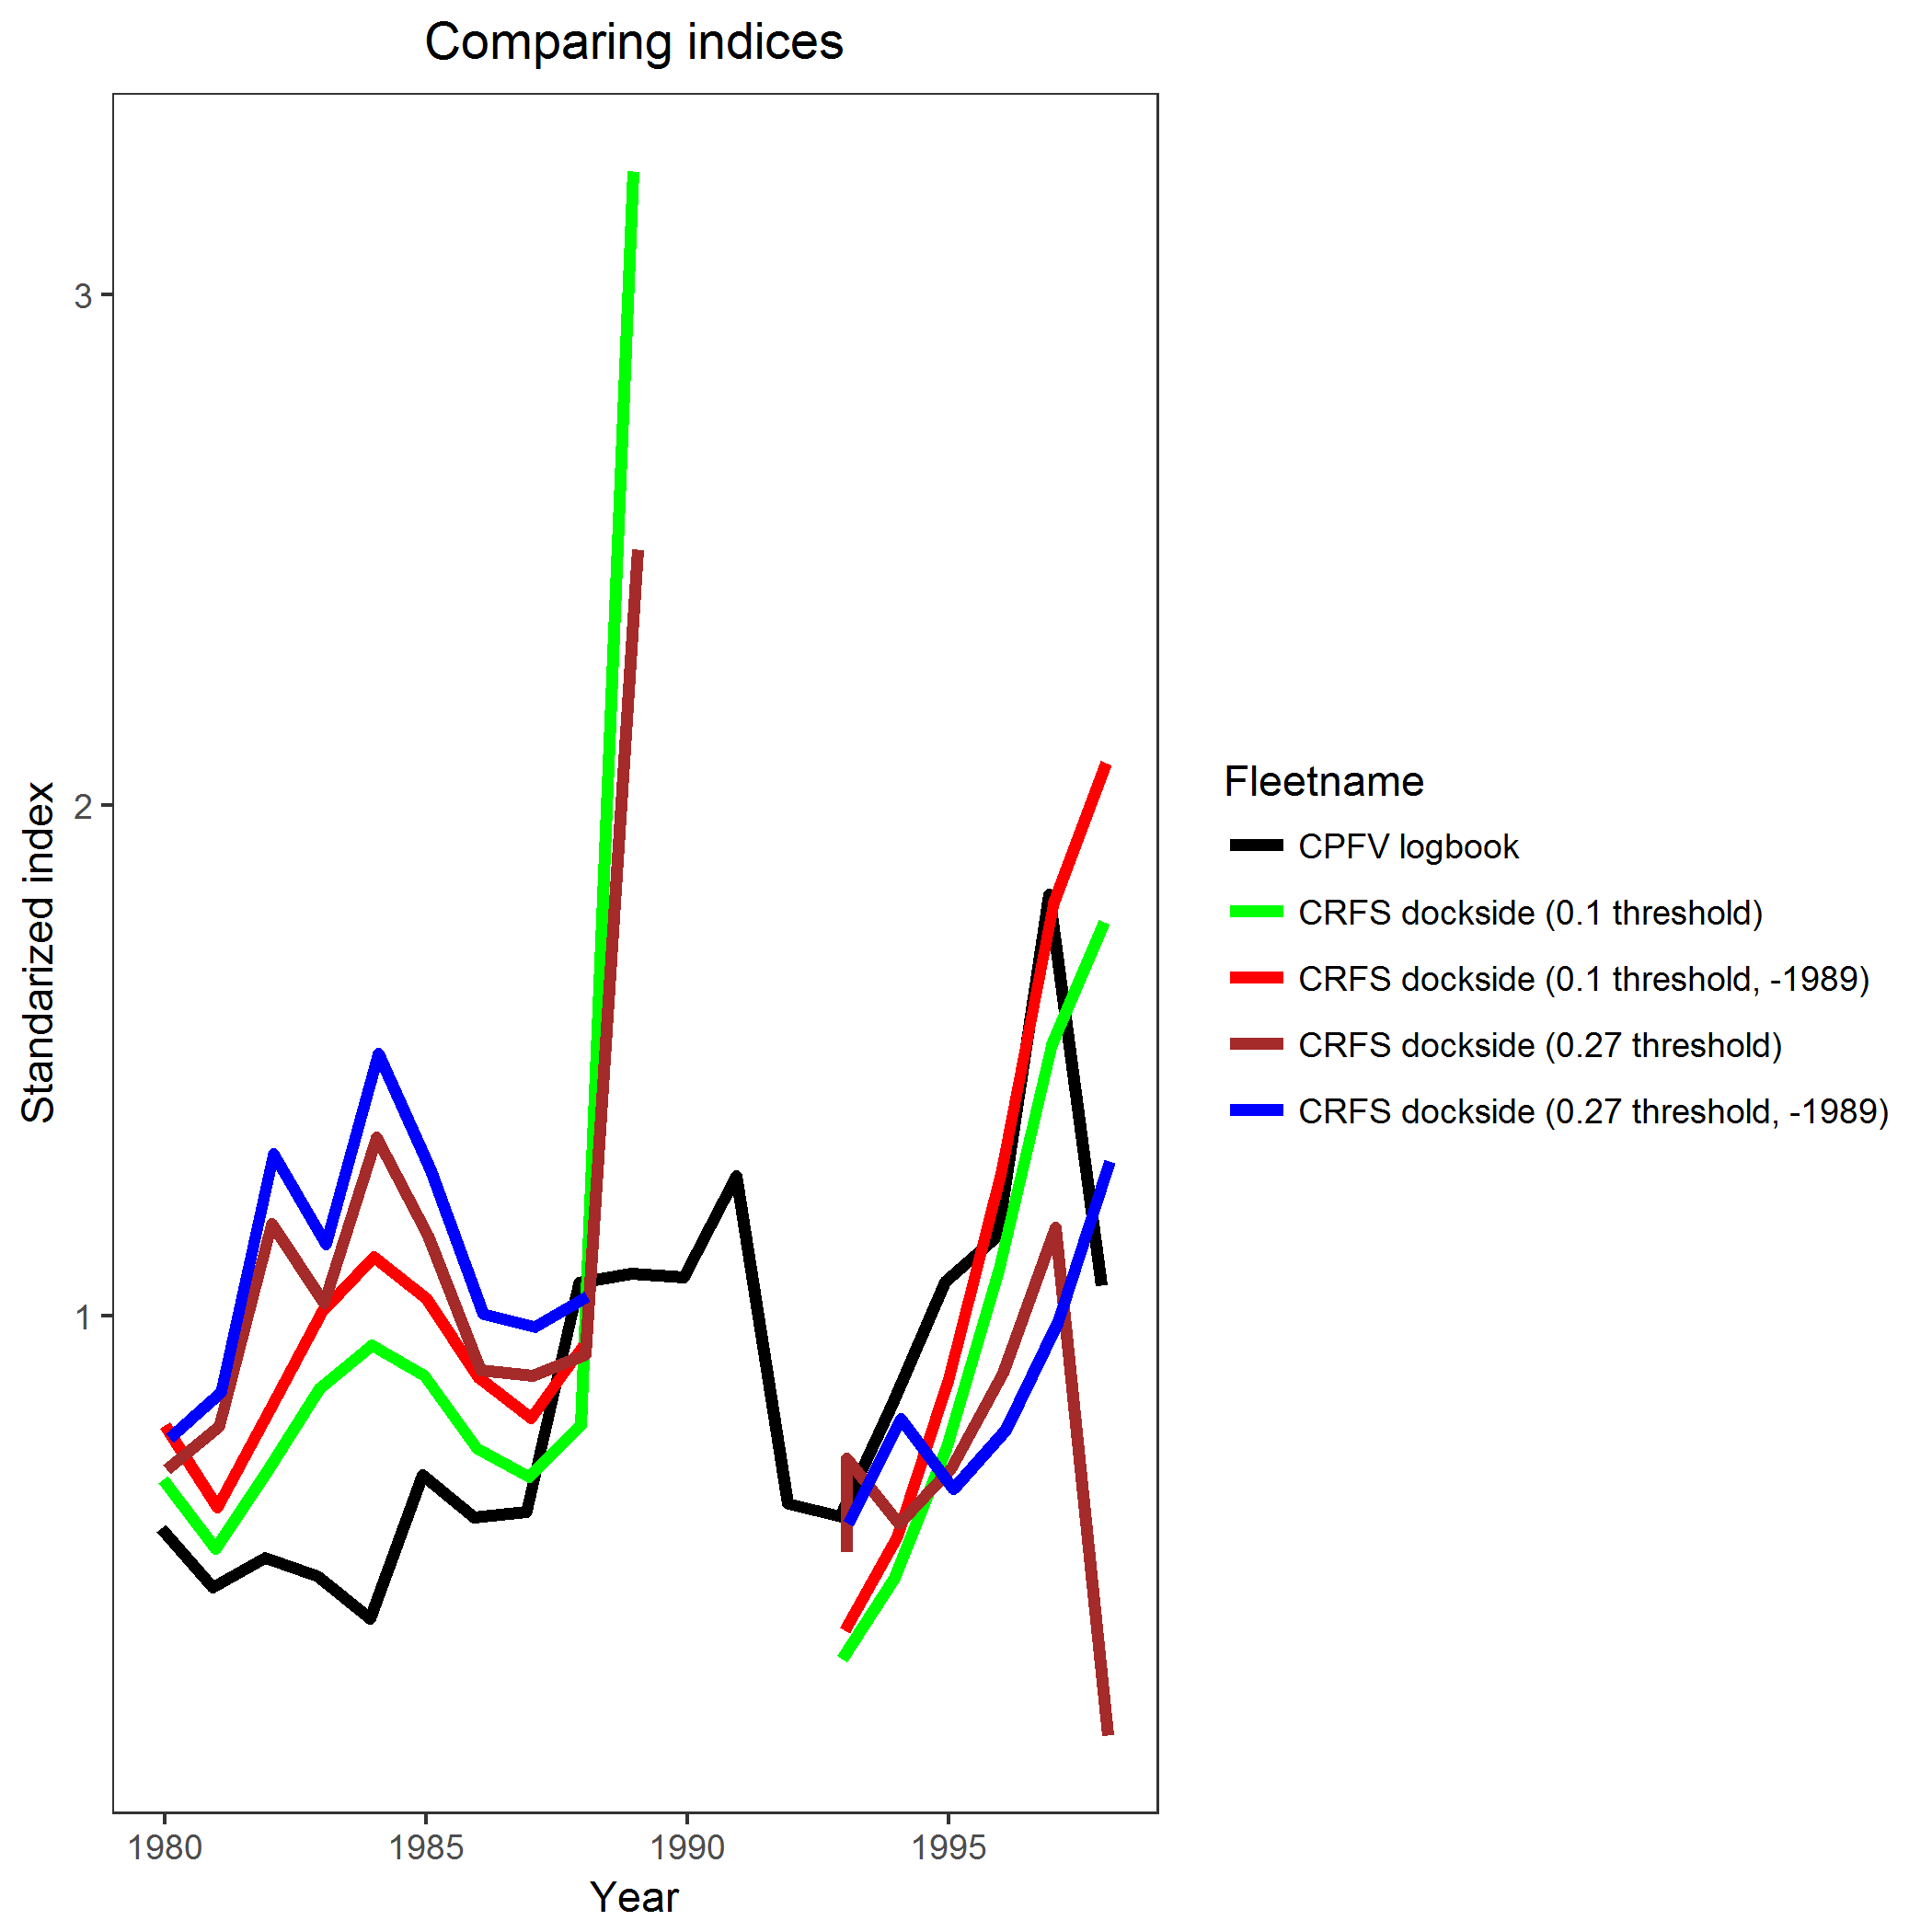
\includegraphics{Figures/Fleet5_RecPC_dockside_index_compare.png}

\endcol
\endcols

\end{frame}

\begin{frame}{Recreational Onboard Indices}

\textbf{Sample}: Drift-level catch \textbf{Years}: 1999-2016
\textbf{Effort}: Angler hours

\begincols
 \begincol{.4\textwidth}

\begin{itemize}
  \item[$\bullet$] Drift-level catch data collection onboard CPFVs
  \item[$\bullet$] Alpha hull method used to select suitable habitat for California scorpionfish
  \item[$\bullet$] Assume that suitable habitat is the same for discarded and retained fish
  \end{itemize}

\endcol
 \begincol{.6\textwidth}

\begin{table}[ht]
\centering
\scalebox{0.5}{
\begin{tabular}{p{1.4in}p{2in}p{.6in}p{.6in}}
  \hline
Filter & Criteria & Pos. trips & Trips \\ 
  \hline
Initial SQL filtering &  & 6,475 & 59,192 \\ 
  Habitat filter & Remove drifts $>$1000 m of alpha hull buffer, remove "reefs" with $<$0 drifts or 5\% positives, or in CCA & 6,365 & 30,987 \\ 
  Exclude 1999 and 2000 & Management changes (depth and gear restrictions) & 5,986 & 29,577 \\ 
  Depth & Remove upper and lower 1\% of data (retain 26-330ft) & 5,921 & 29,002 \\ 
  Minutes Fished & Remove upper and lower 1\% of data (retain 4 - 155 minutes) & 5,780 & 28,460 \\ 
  Observed Anglers & Remove upper and lower 1\% of data (retain 4 - 15 anglers) & 5,679 & 27,946 \\ 
  Boats  & Include boats encountering scorpionfish in at least 3 years; at least 30 drifts and 10 with scorpionfish & 5,509 & 26,805 \\ 
  Second depth filter & Remove anything $>$100 m after looking at 20 m depth bins & 5,507 & \textbf{26,733} \\ 
   \hline
\end{tabular}
}
\end{table}

\endcol
\endcols

\end{frame}

\begin{frame}{Recreational Onboard Indices}

\vspace{1cm}

\begincols
 \begincol{.5\textwidth} Discarded Catch

\begin{table}[ht]
\centering
\scalebox{0.6}{
\begin{tabular}{p{2in}p{.6in}p{.6in}}
  \hline
Model & Binomial & Lognormal \\ 
  \hline
~Year & 19619 & 9177 \\ 
  ~Year + Reef & 18677 & 9177 \\ 
  ~ Year + Depth & 19374 & 8860 \\ 
  ~Year + Depth + Reef & 18392 & 8778 \\ 
  ~Year + Month + Reef + Depth & \textbf{18318} & \textbf{8769} \\ 
   \hline
\end{tabular}
}
\end{table}

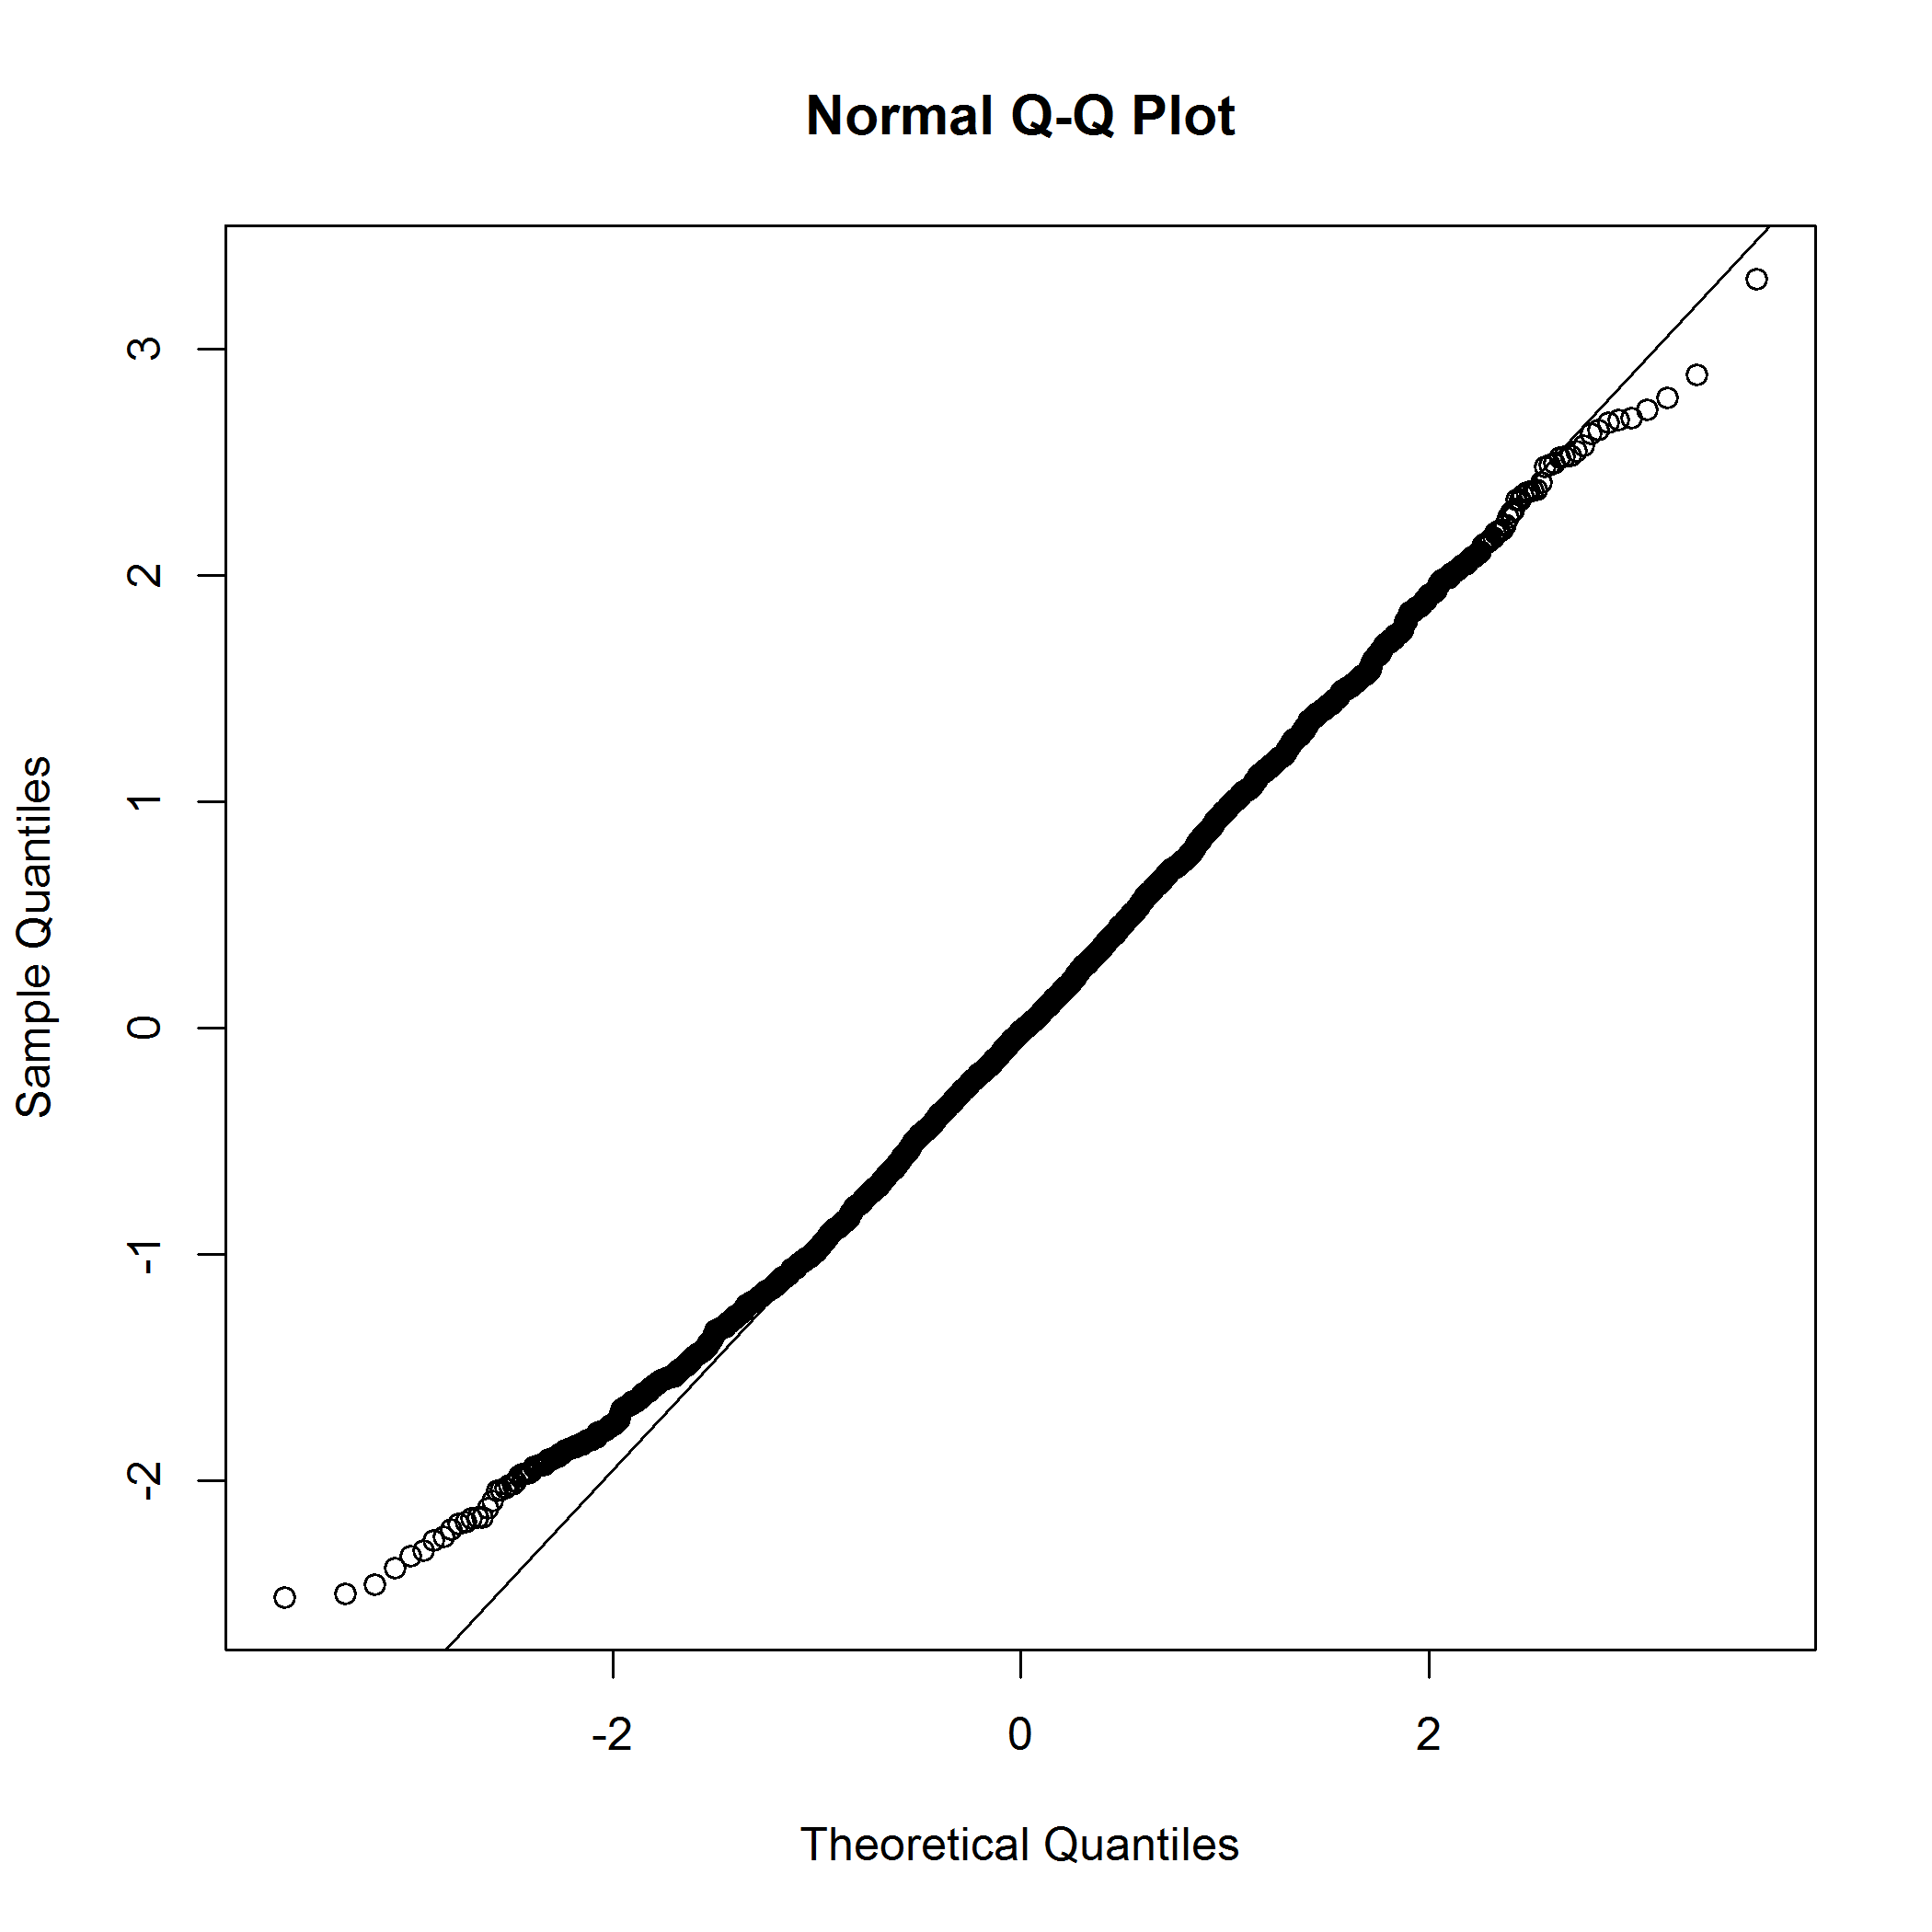
\includegraphics[height=4cm]{Figures/Fleet6_RecDD_QQ.png}

\endcol
 \begincol{.5\textwidth}

Retained Catch

\begin{table}[ht]
\centering
\scalebox{0.6}{
\begin{tabular}{p{2in}p{.6in}p{.6in}}
  \hline
Model & Binomial & Lognormal \\ 
  \hline
~Year & 21826 & 11507 \\ 
  ~Year + Reef & 21192 & 11325 \\ 
  ~ Year + Depth & 21265 & 10704 \\ 
  ~Year + Depth + Reef & 20691 & 10619 \\ 
  ~Year + Month + Reef + Depth & \textbf{20453} & \textbf{10599} \\ 
   \hline
\end{tabular}
}
\end{table}

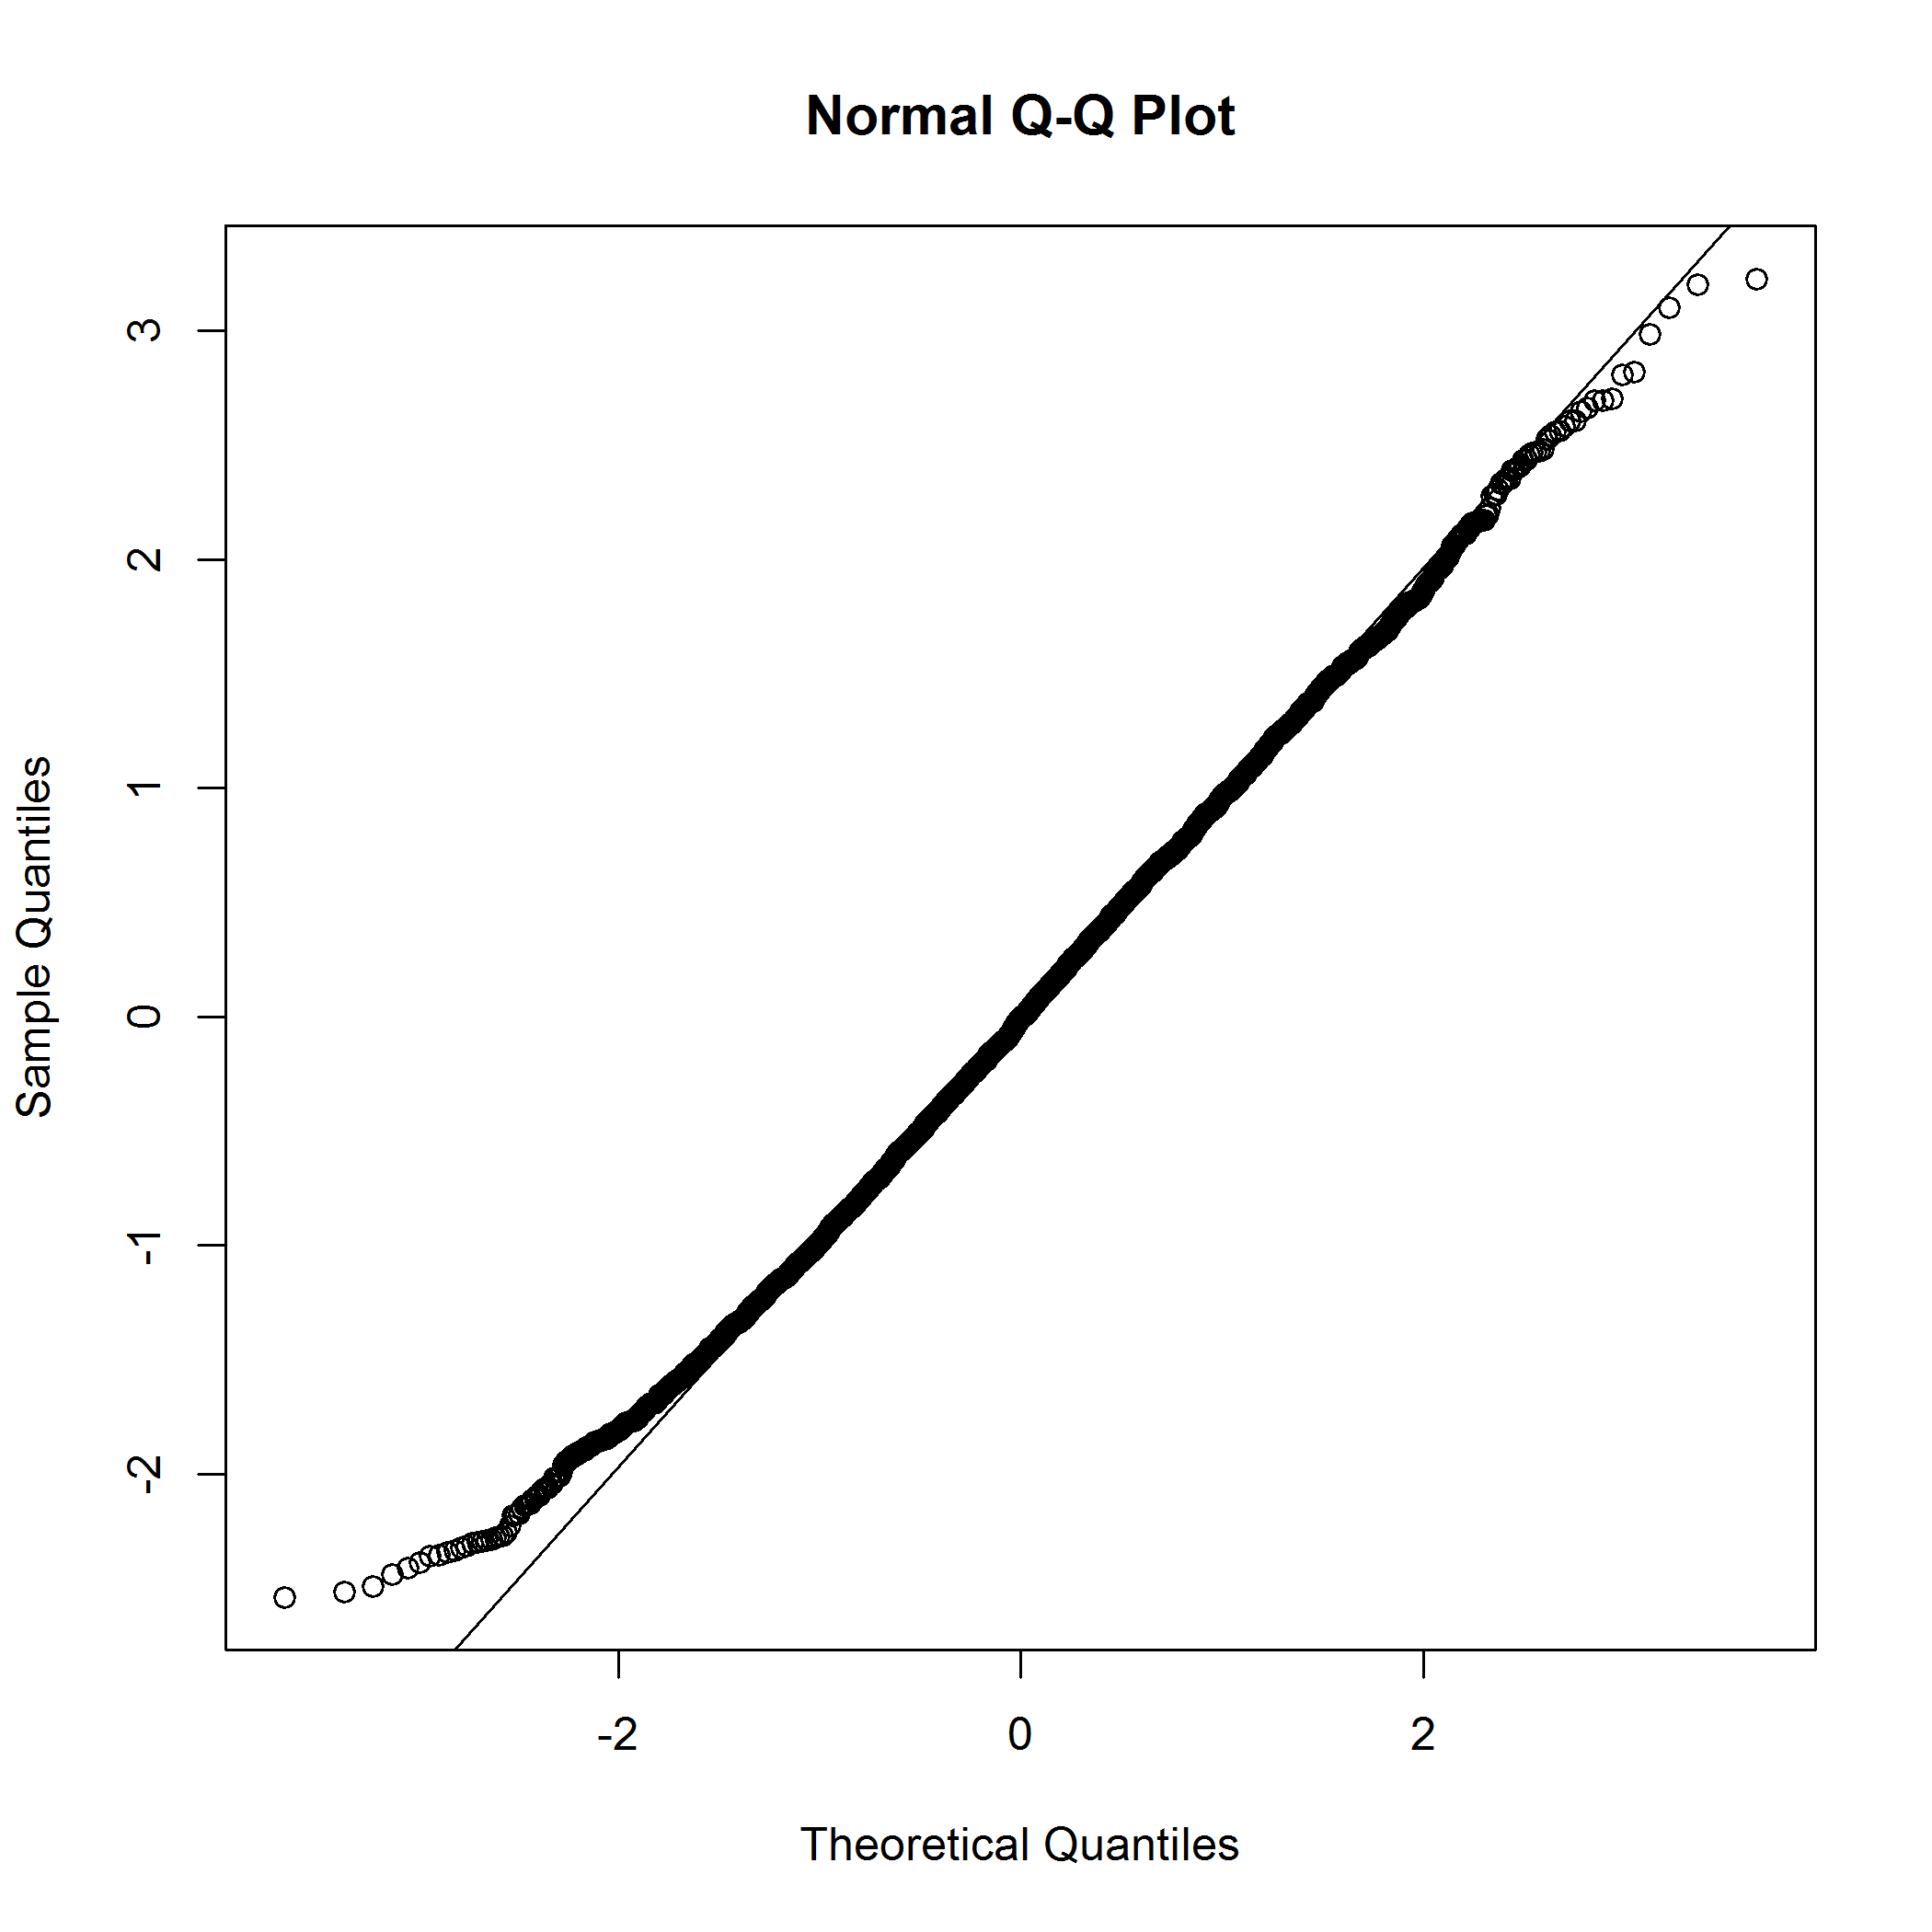
\includegraphics[height=4cm]{Figures/Fleet12_RecPCOB_QQ.png} \endcol
\endcols

\end{frame}

\begin{frame}{Recreational Onboard Indices}

\begincols
 \begincol{.5\textwidth} Discard catch index (left)
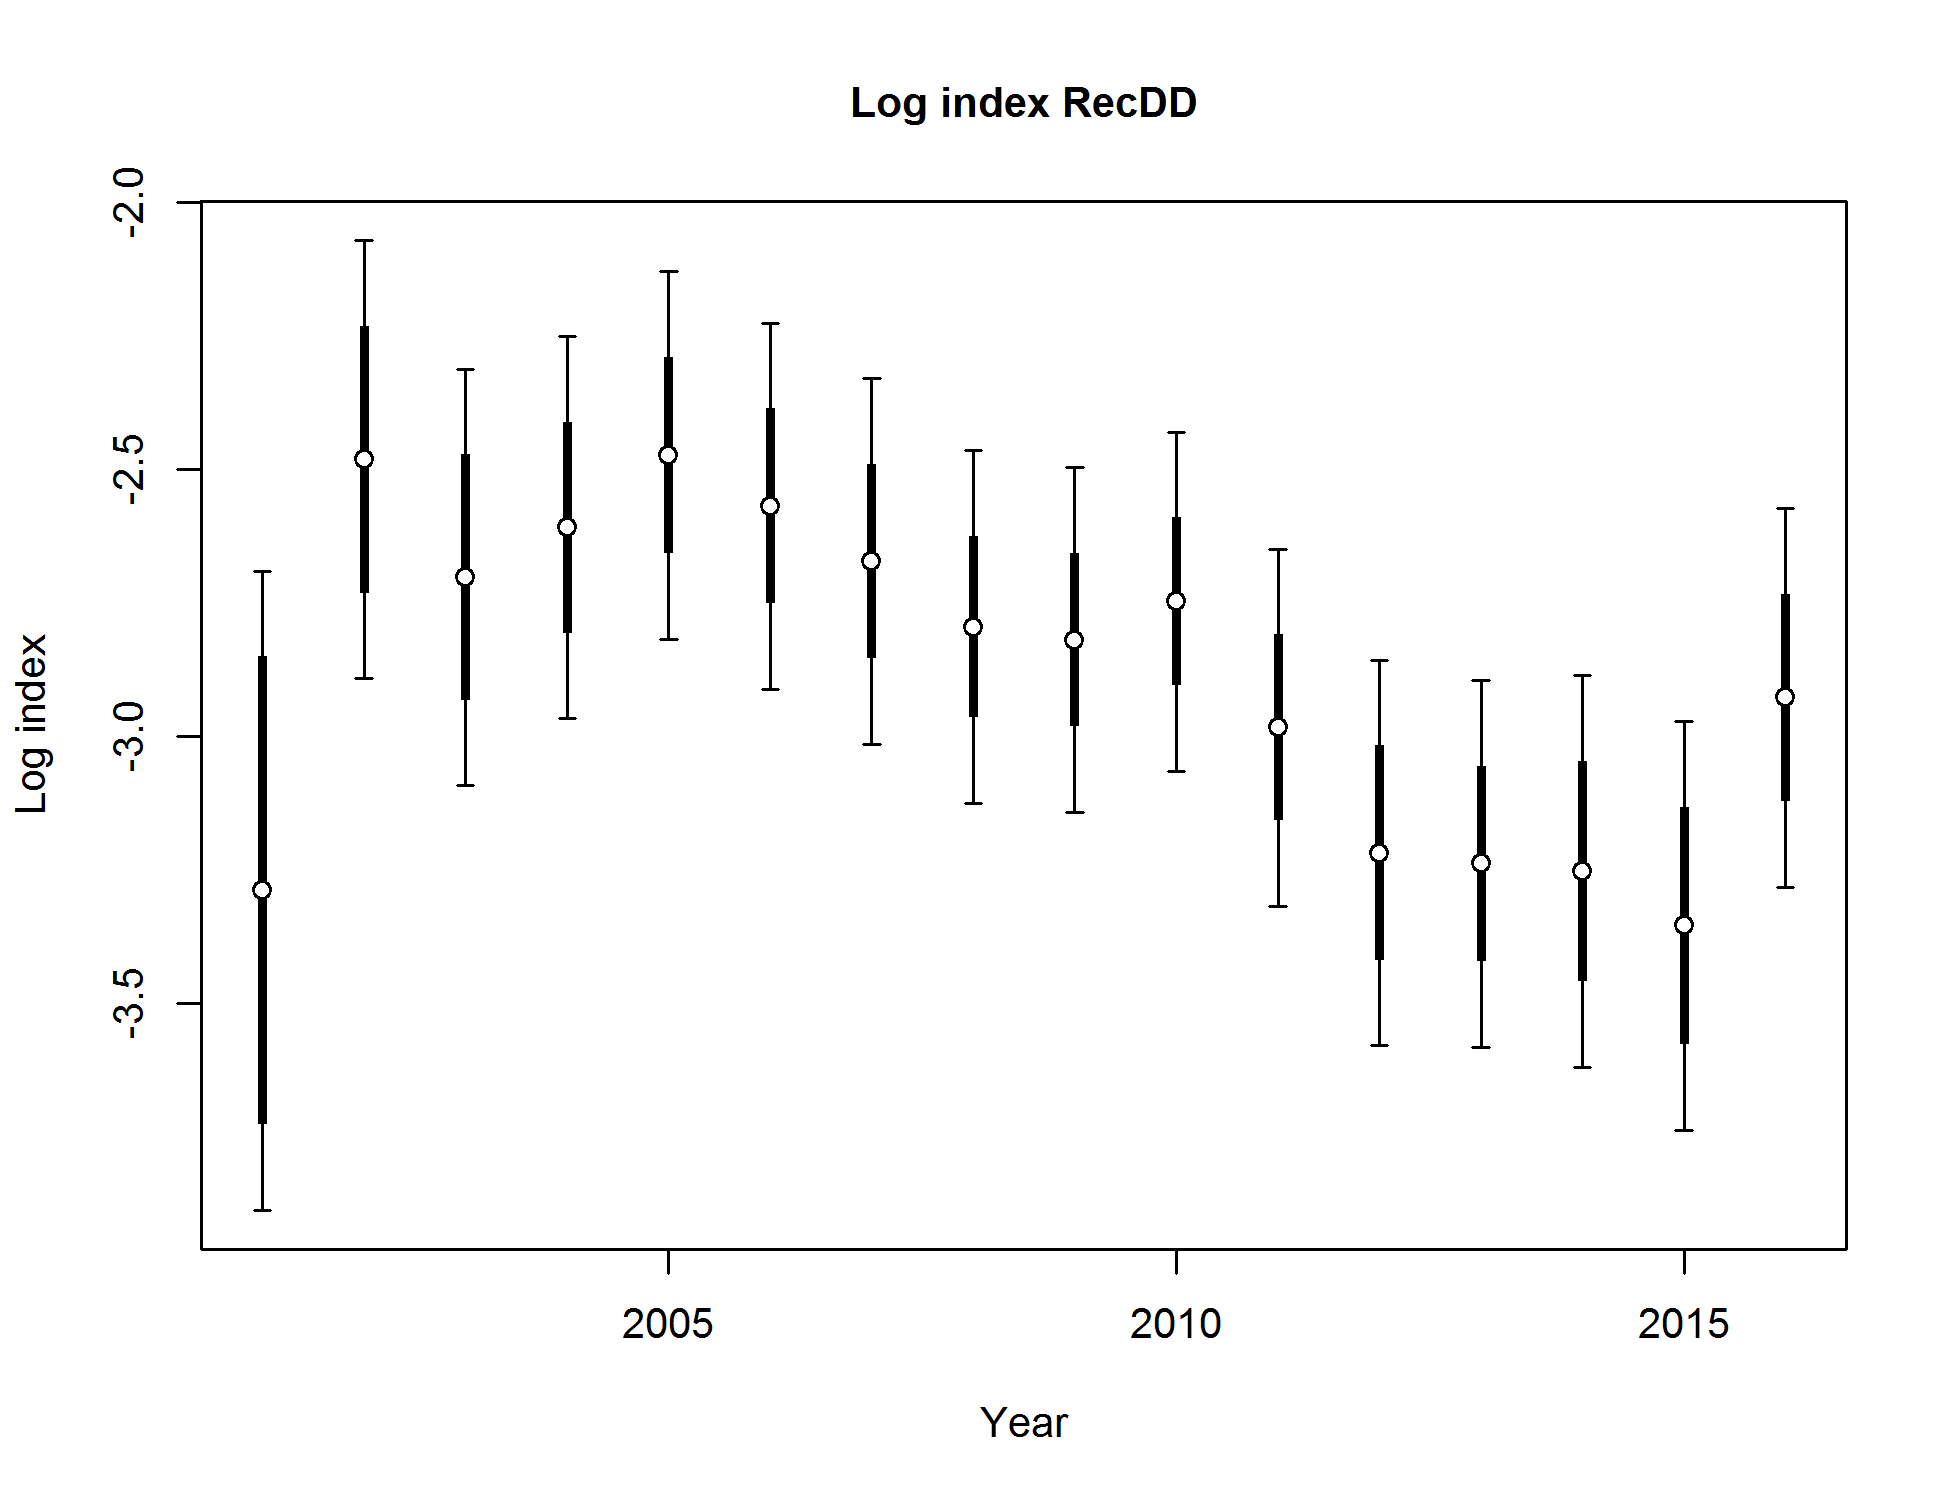
\includegraphics{r4ss/plots_mod1/index4_logcpuedata_RecDD.png}

\endcol
 \begincol{.5\textwidth} Retained catch index (right)
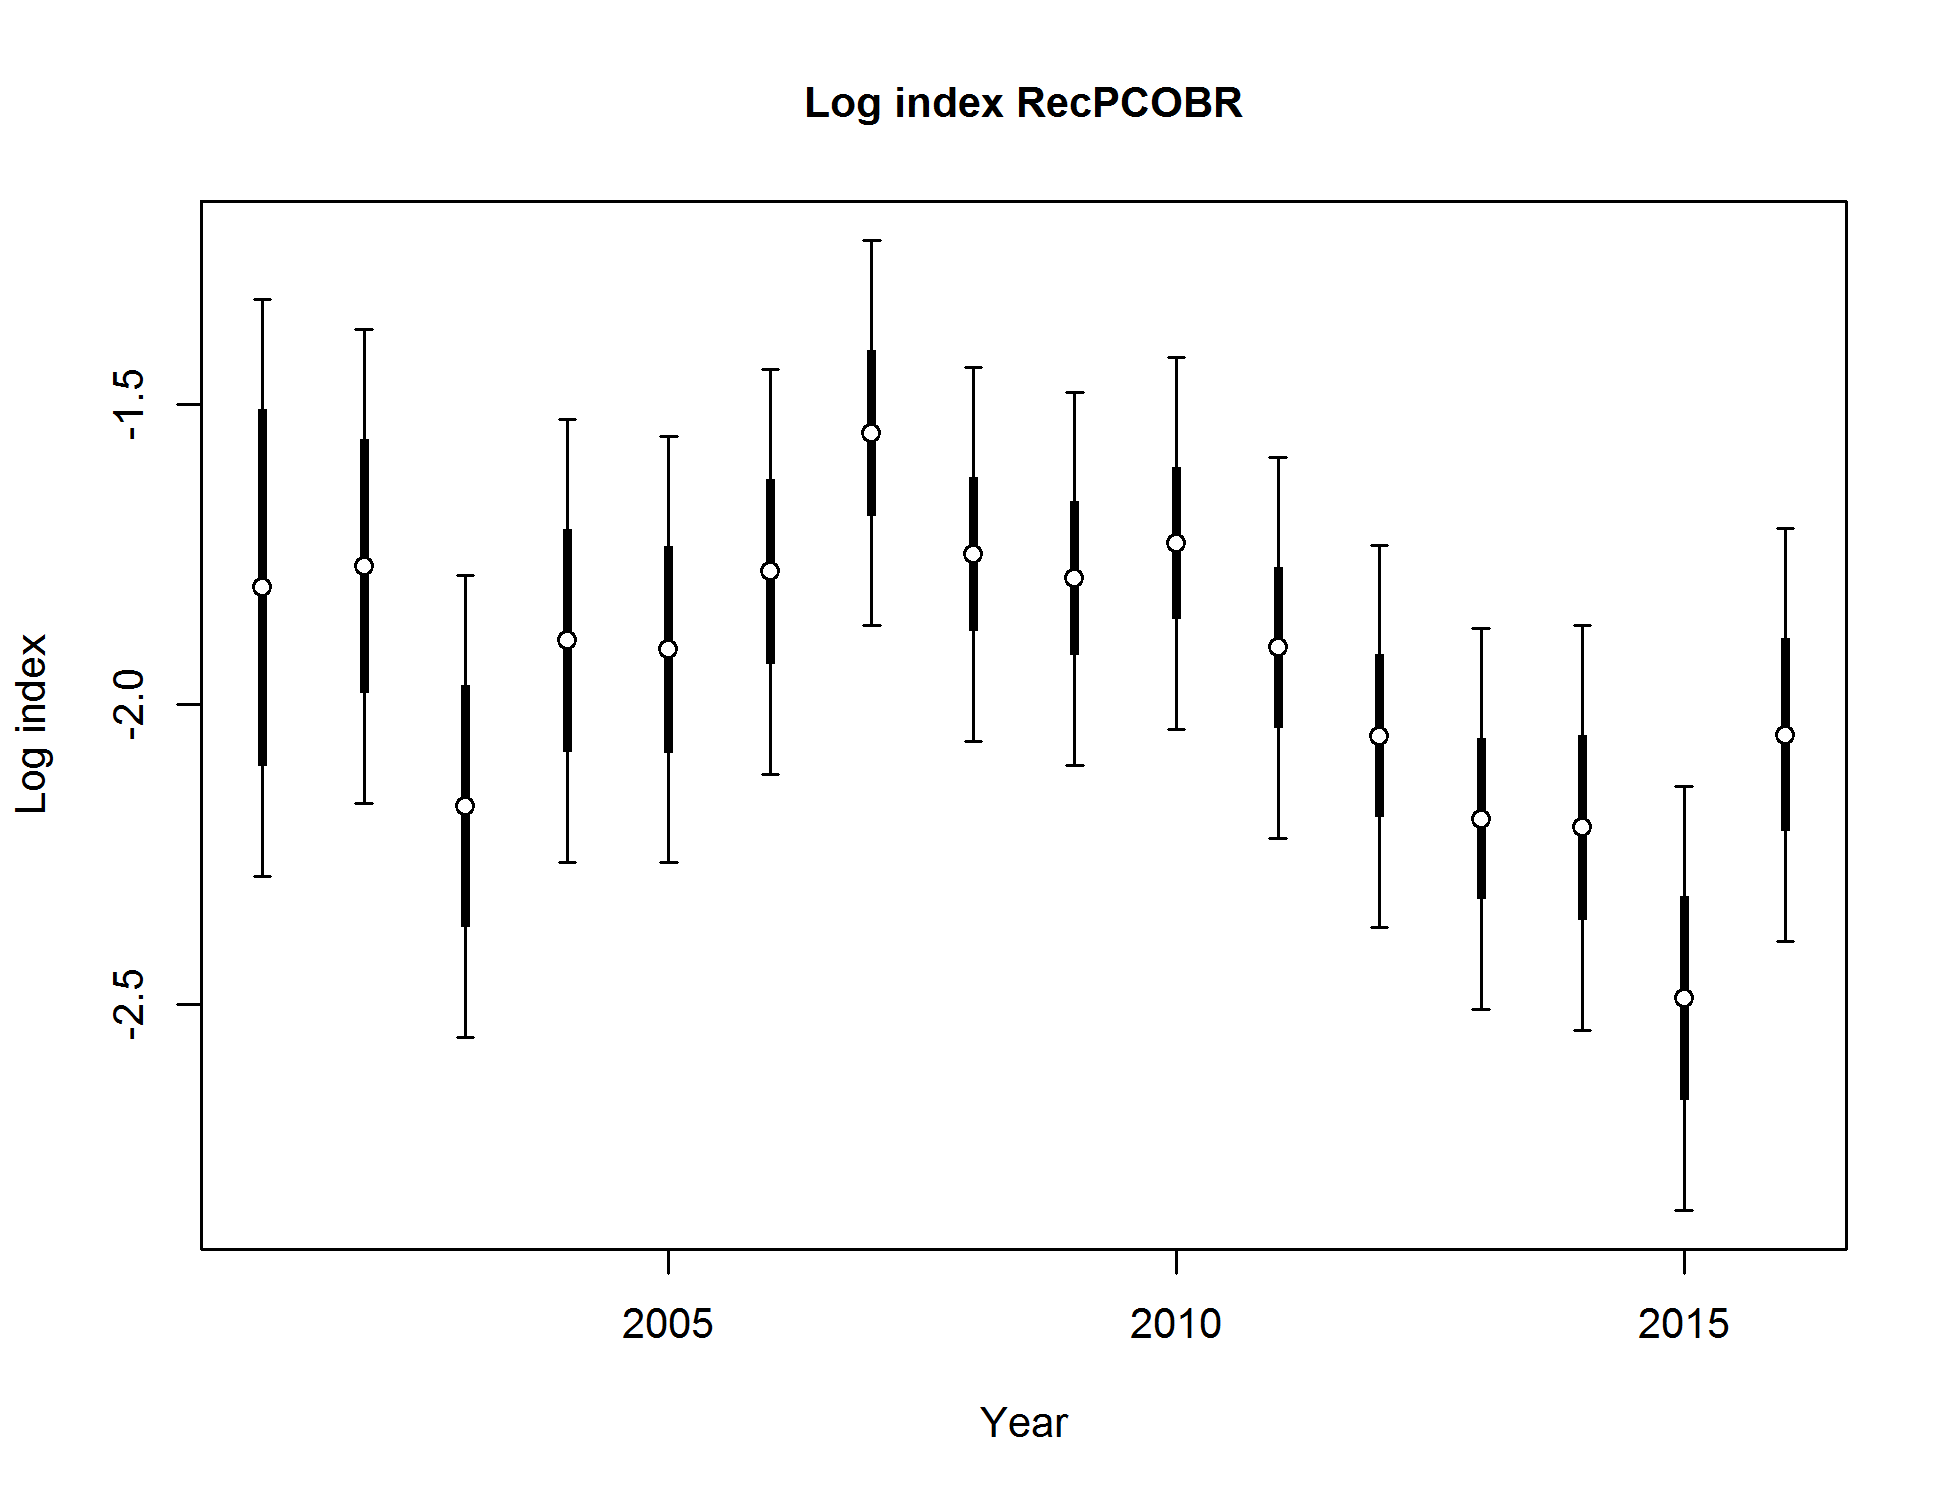
\includegraphics{r4ss/plots_mod1/index4_logcpuedata_RecPCOBR.png}
\endcol
\endcols

\end{frame}

\begin{frame}{Recreational Onboard Indices}

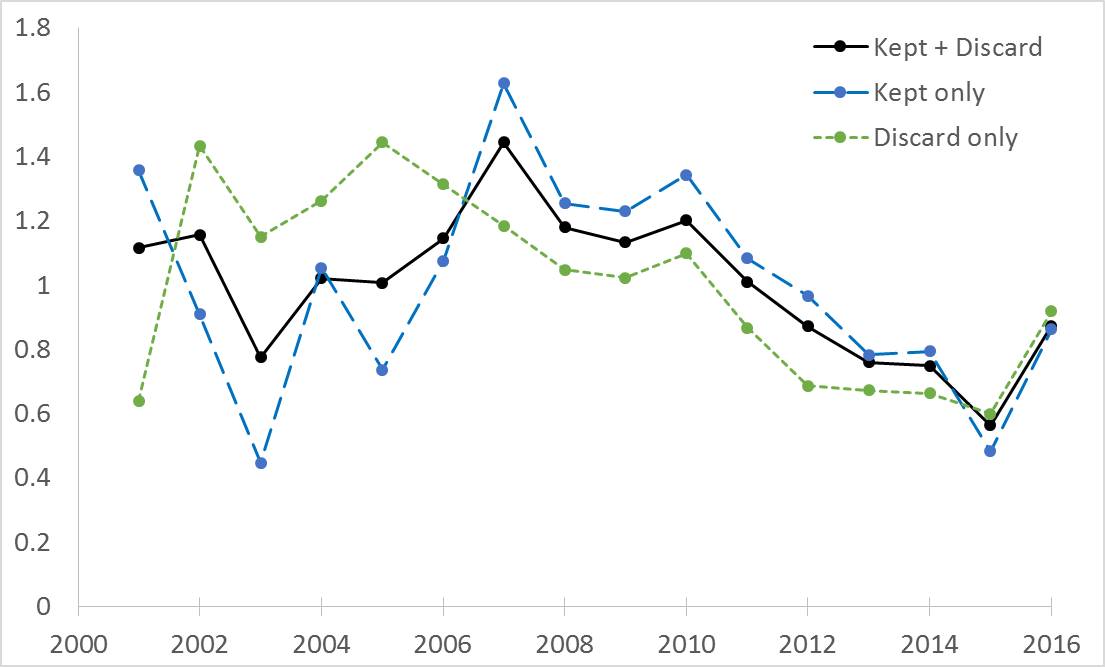
\includegraphics{Figures/Fleets6_12_index_compare.png}

\end{frame}

\begin{frame}{Fishery-Independent Abundance Indices}

\begin{itemize}
\item[$\bullet$] Publicly Owned Treatment Works (POTW) Monitoring Index
\item[$\bullet$] NWFSC Trawl Survey 
\item[$\bullet$] California State Univeristy Northridge/Vantuna Research Group (CSUN/VRG) Gillnet Survey
\item[$\bullet$] Generating Station Impingement Survey
\item[$\bullet$] Southern California Bight Regional Monitoring Survey (Bight survey)
\end{itemize}

\end{frame}

\begin{frame}{Publicly Owned Treatment Works Survey Index}

\begin{itemize}
\item[$\bullet$] Publicly Owned Treatment Works (POTWs) are required to have permits to discharge into state or federal waters
\item[$\bullet$] Six southern California POTWs conduct trawls to monitoring fish populations (Goleta and City of Oxnard do not observer California scorpionfish)
\begin{itemize}
\item[$\circ$] Each POTW follows standardized trawl methods
\item[$\circ$] Fixed station design, sample spring and fall, or more frequently
\item[$\circ$] All fish encountered are measured, standard length
\end{itemize}
\item[$\bullet$]  Four POTWs observed California scorpionfish
\begin{itemize}
\item[$\circ$] Orange County Sanitation District (1970-2016)
\item[$\circ$] City of Los Angeles Environmental Monitoring Division (1988-2016)
\item[$\circ$] Sanitation Districts of Los Angeles County (1972-2016)
\item[$\circ$] City of San Diego Public Utilities Department (1985-2016)
\end{itemize}
\end{itemize}

\end{frame}

\begin{frame}{POTW Survey Index}

\begincols
 \begincol{.5\textwidth} \centering
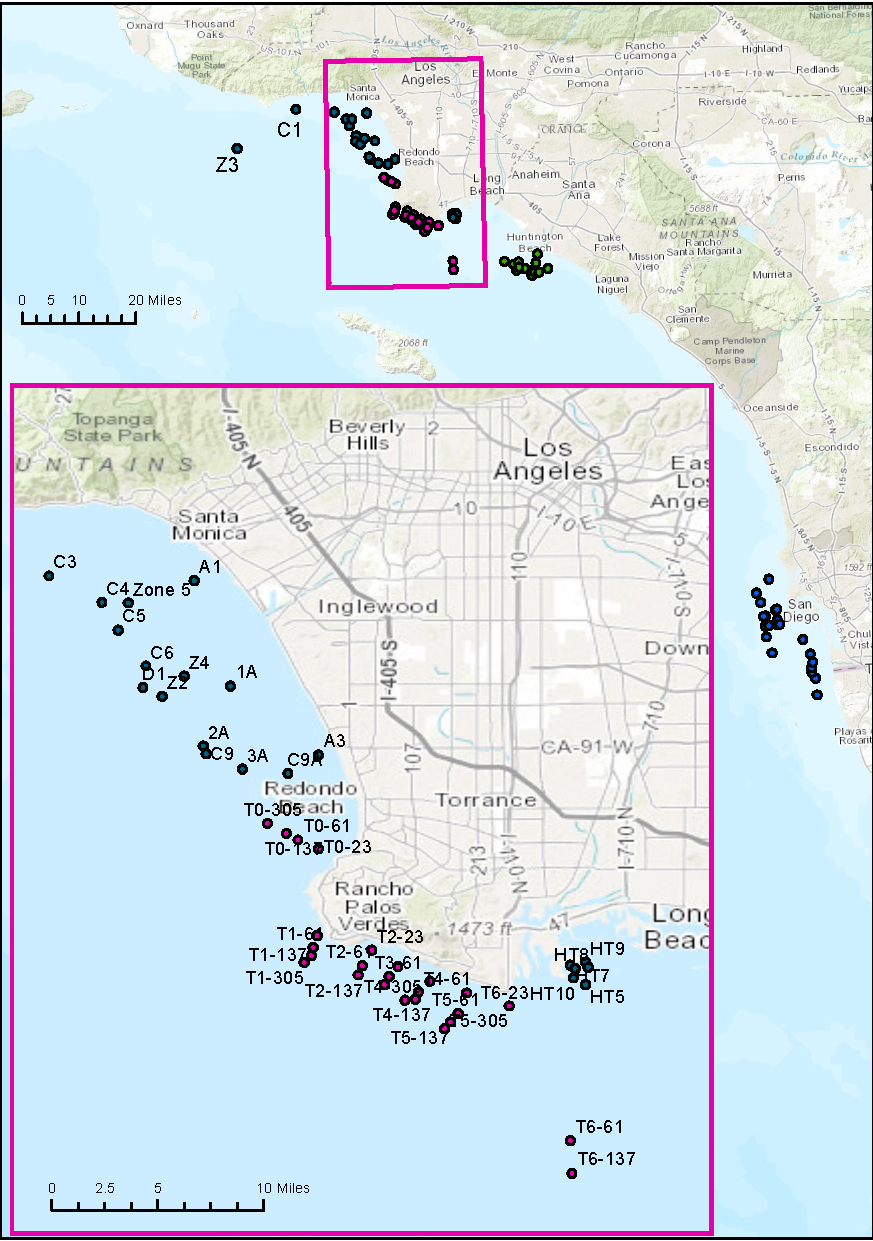
\includegraphics{Figures/Fleet7_sanitation_map2.pdf} \endcol
 \begincol{.5\textwidth} \centering
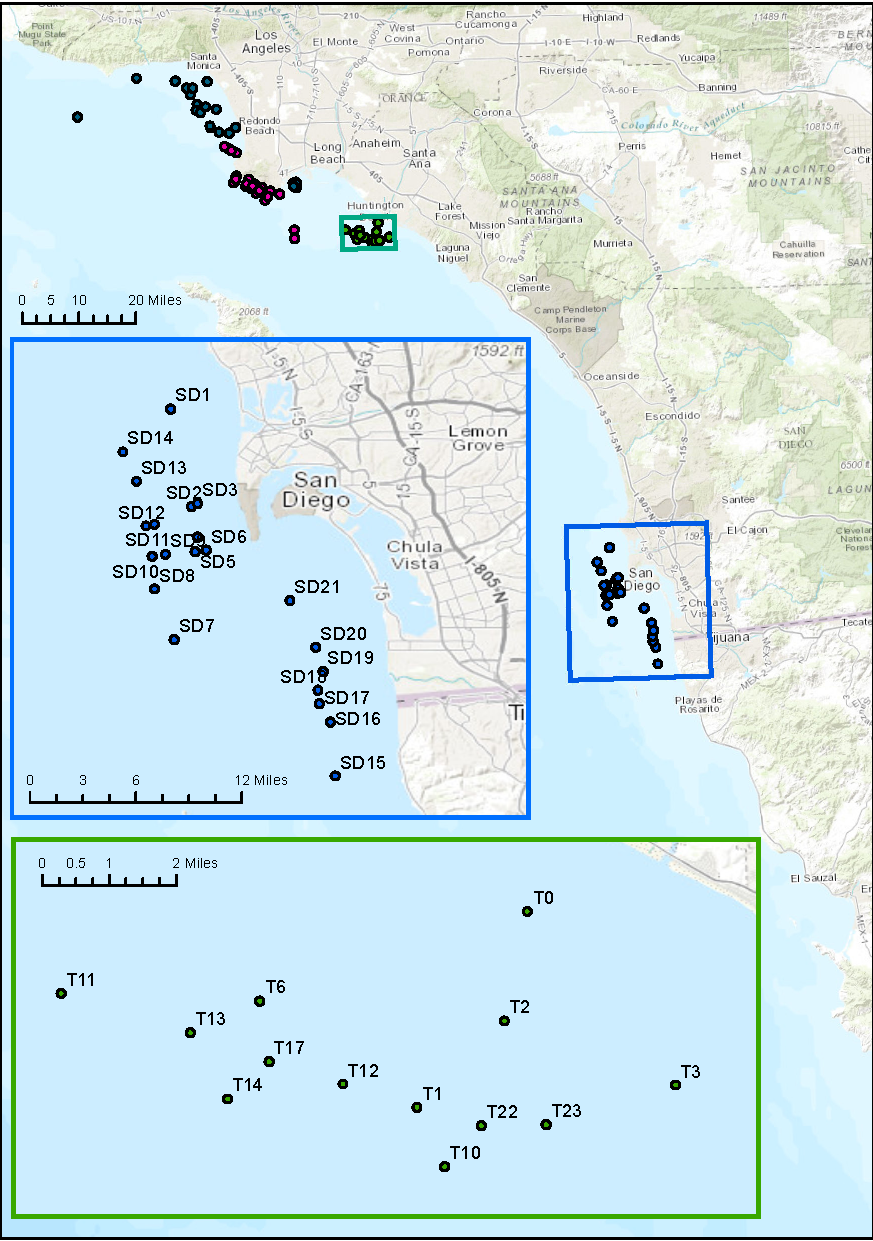
\includegraphics{Figures/Fleet7_sanitation_map1.pdf} \endcol
\endcols

\end{frame}

\begin{frame}{Publicly Owned Treatment Works Survey Index}

\textbf{Sample}: Four POTWs \textbf{Years}: 1970-2016 \textbf{Effort}:
Tow time

Number of California scorpionfish encountered by POTW and 25 m depth bin

\begin{table}[ht]
\centering
\scalebox{0.9}{
\begin{tabular}{lrrrrr}
  \hline
Program & 0-24 m & 25-49 m & 50-74 m & 100+ m & Total \\ 
  \hline
City of Los Angeles & 120 &   0 & 1372 &   0 & 1492 \\ 
  Los Angeles County & 687 &   0 & 5879 & 450 & 7016 \\ 
  Orange County & 161 & 669 & 2157 &  48 & 3035 \\ 
  City of San Diego &   0 & 404 & 333 & 829 & 1566 \\ 
   \hline
\end{tabular}
}
\end{table}

\end{frame}

\begin{frame}{Publicly Owned Treatment Works Survey Index}

\textbf{Results}

\begincols
 \begincol{.4\textwidth}
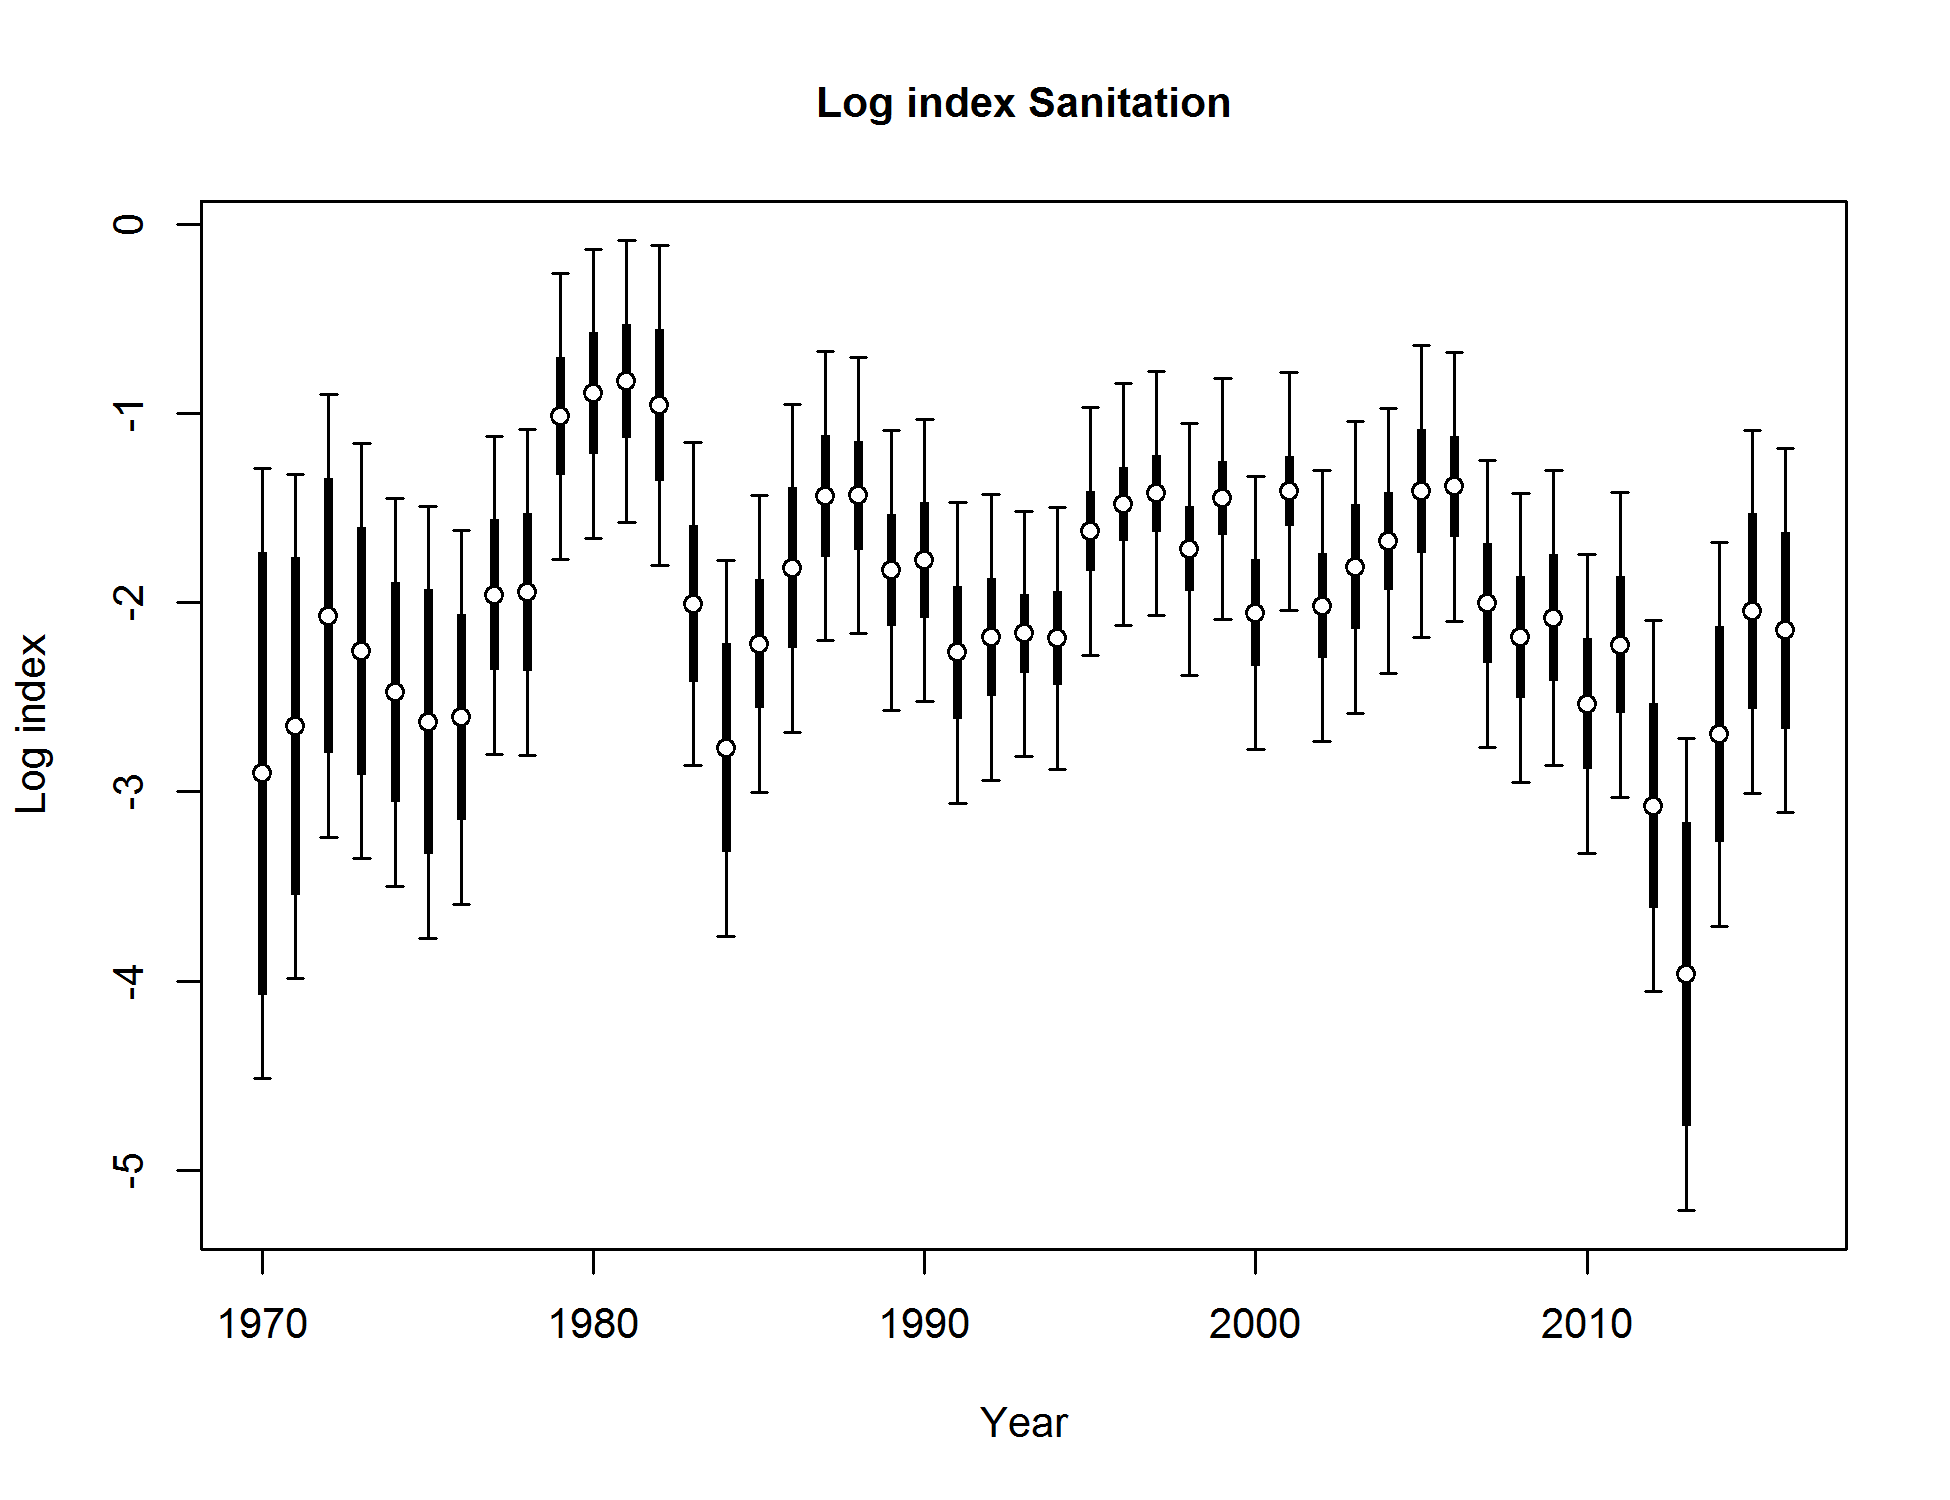
\includegraphics{r4ss/plots_mod1/index4_logcpuedata_Sanitation.png}
\endcol
 \begincol{.6\textwidth}
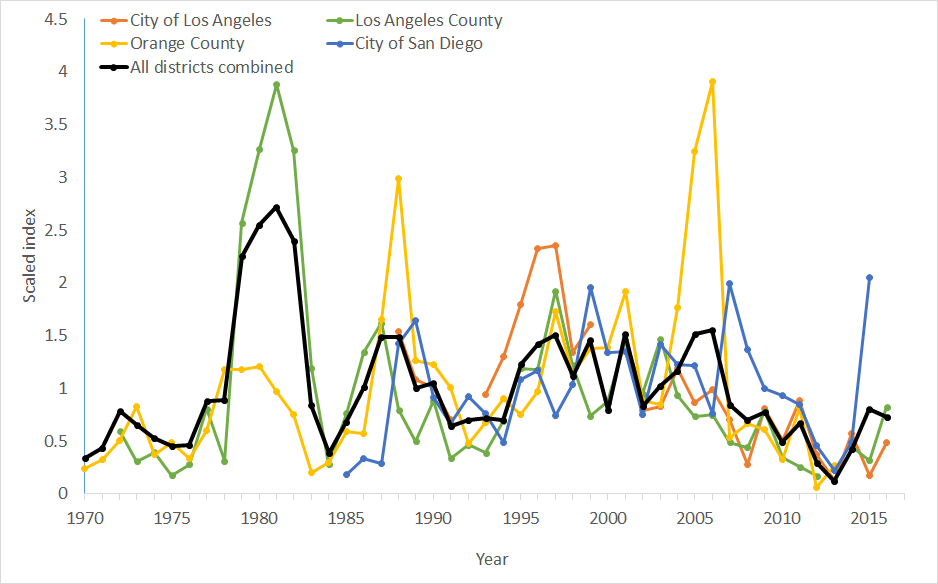
\includegraphics{Figures/Fleet7_Sanitation_indexcompare.png}

\endcol
\endcols

\end{frame}

\begin{frame}{Gillnet Survey Index}

\textbf{Sample}: CSUN/VRG survey \textbf{Years}: 1995-2008
\textbf{Effort}: Soak time

\begincols
 \begincol{.6\textwidth}

\begin{table}[ht]
\centering
\scalebox{0.5}{
\begin{tabular}{p{1.4in}p{2in}p{.6in}p{.6in}}
  \hline
Filter & Criteria & Pos. trips & Trips \\ 
  \hline
Entire dataset &  & 325 & 3,558 \\ 
  General data filters & Samples with  no net failures & 269 & 3,515 \\ 
  Net type & Samples using a net type 1", 1.5" and 2" mesh & 269 & 2,815 \\ 
  Sites & Sites frequently sampled & 266 & 2,170 \\ 
  Month & Months sampled consistently (April, June, August, October) & 259 & 2,019 \\ 
   \hline
\end{tabular}
}
\end{table}

\begin{table}[ht]
\centering
\scalebox{0.5}{
\begin{tabular}{p{3in}p{.6in}p{.6in}}
  \hline
Model & Binomial & Lognormal \\ 
  \hline
~Year + month + site + perp\_para + floats & 1983 & 1008 \\ 
  ~Year + site + perp\_para  + floats & 2000 & 1004 \\ 
   Year + month  + perp\_para + floats & 2349 & 1264 \\ 
  ~Year  + site +  perp\_para & \textbf{2010} & \textbf{1004} \\ 
   \hline
\end{tabular}
}
\end{table}

\endcol
 \begincol{.4\textwidth}

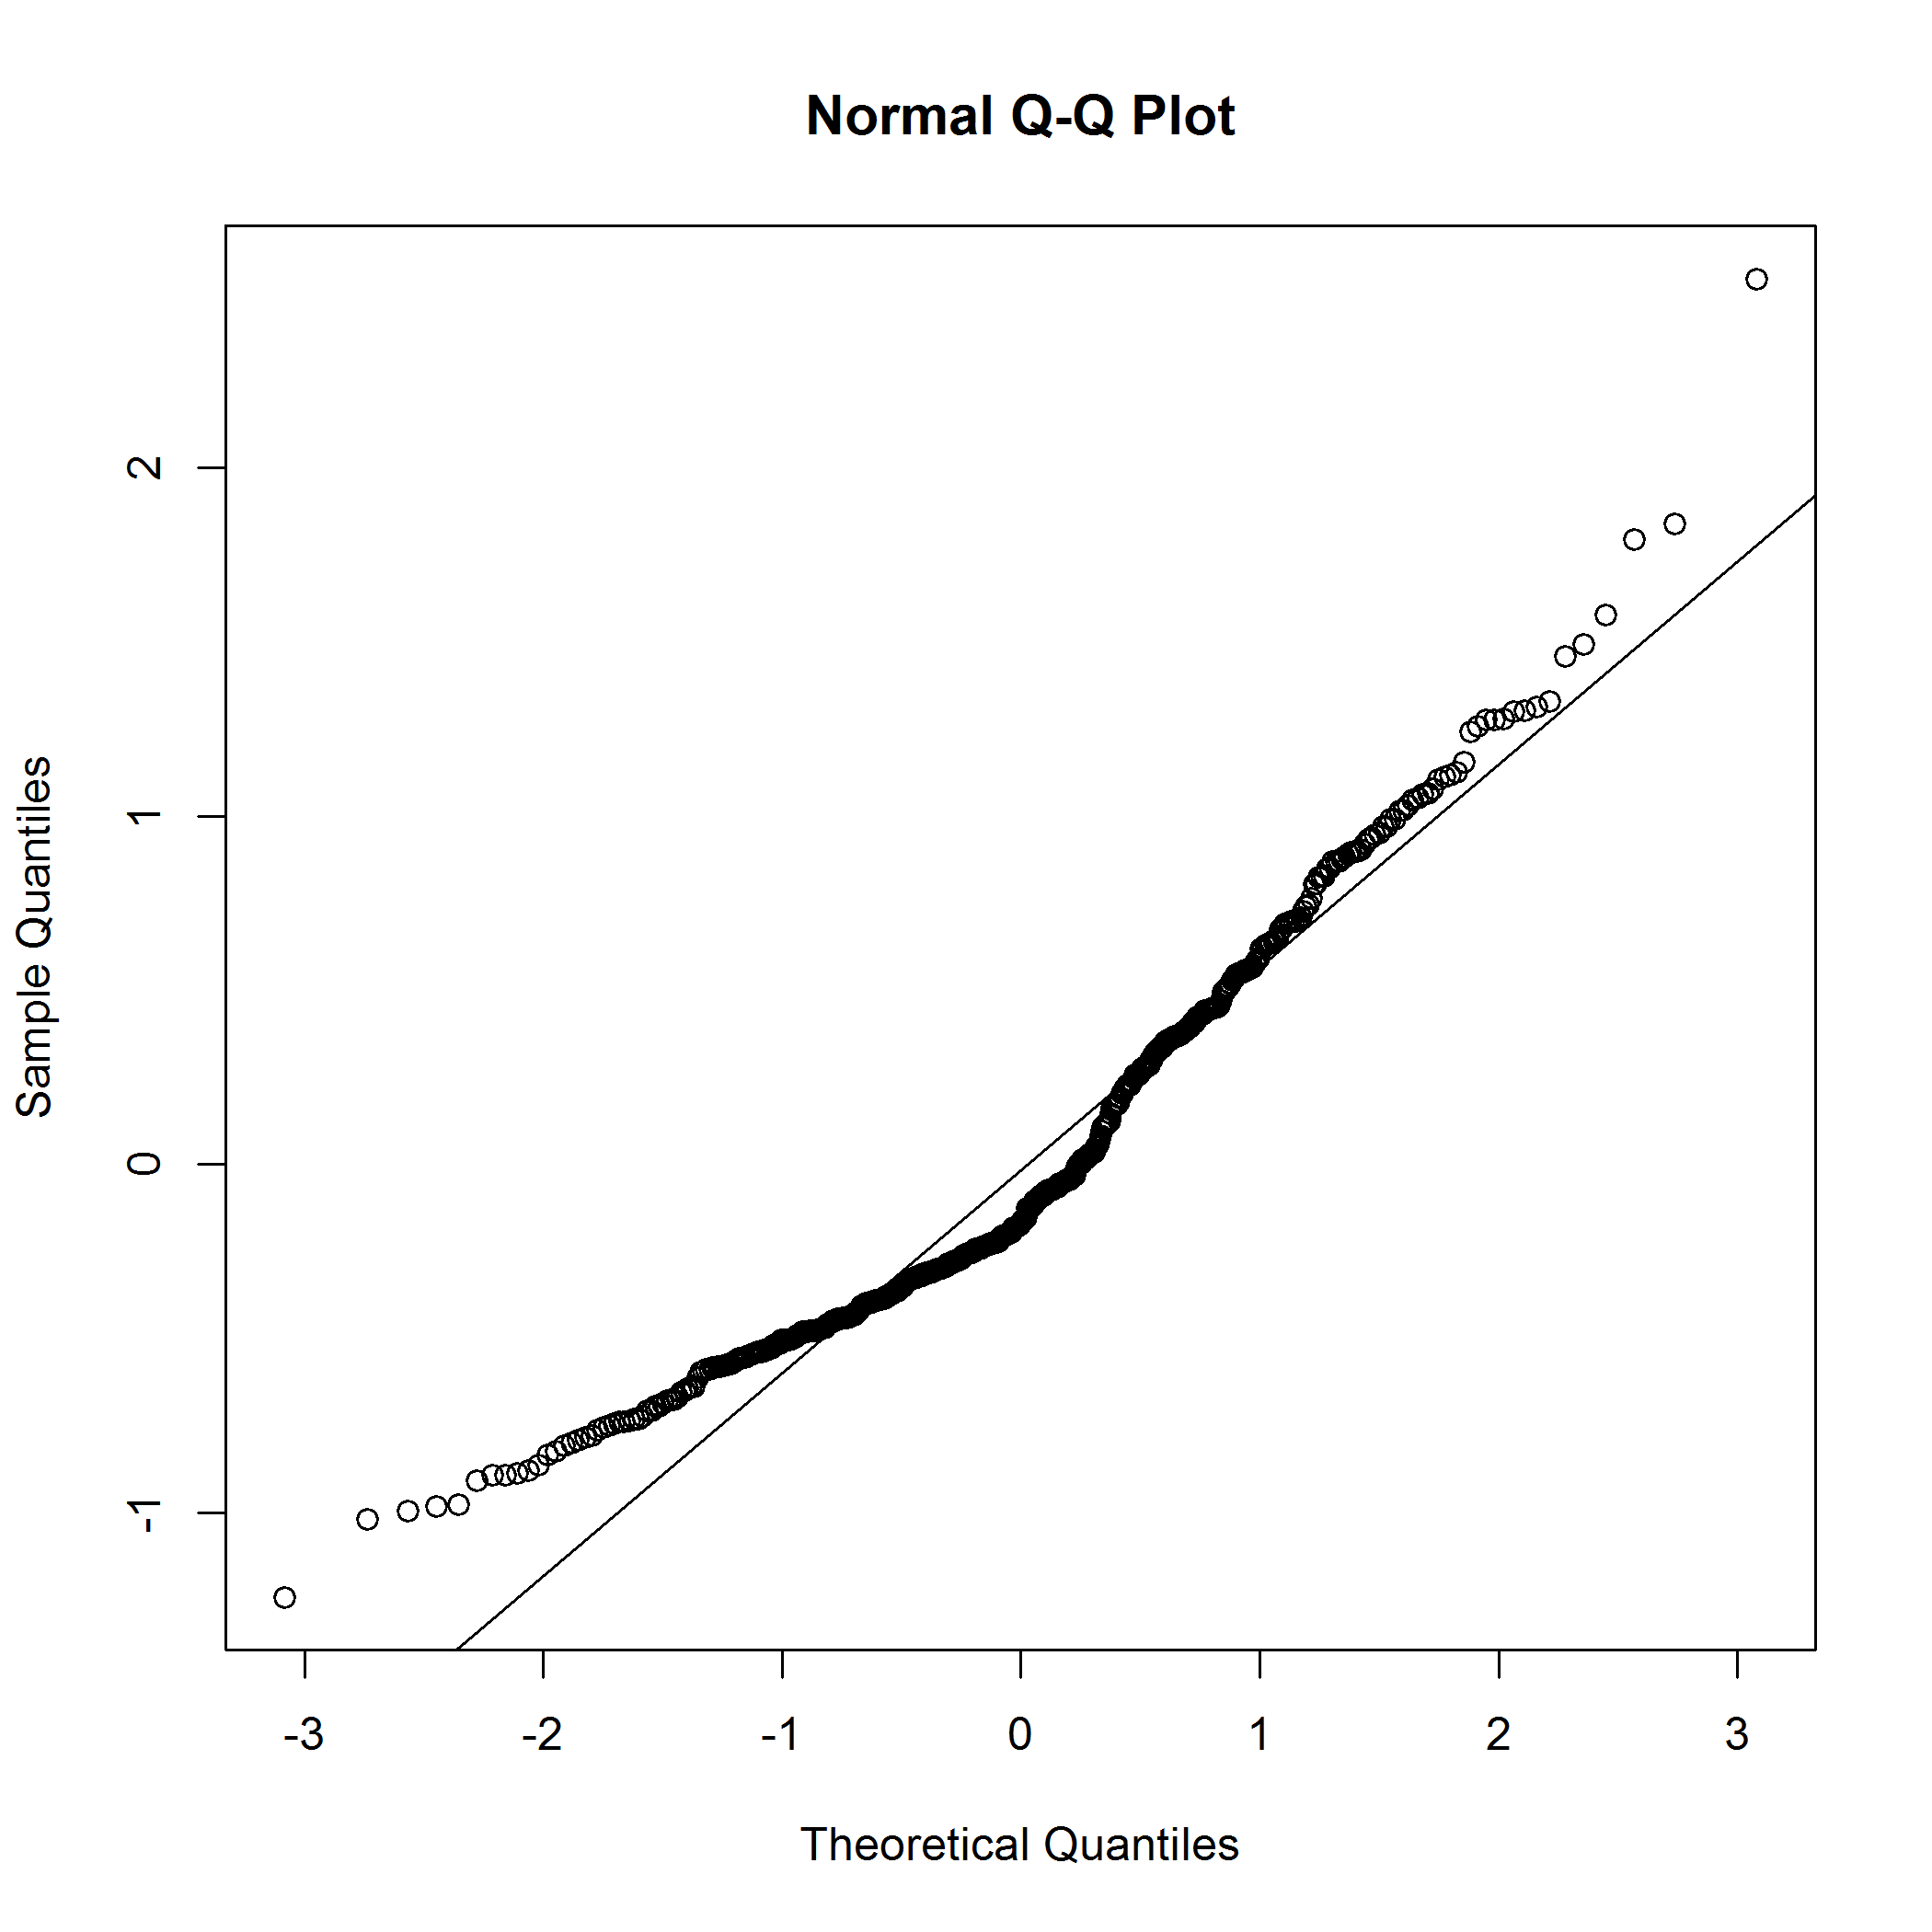
\includegraphics[height=5cm]{Figures/Fleet9_GillnetSurvey_QQ.png}

\endcol
\endcols

\end{frame}

\begin{frame}{Gillnet Survey Index}

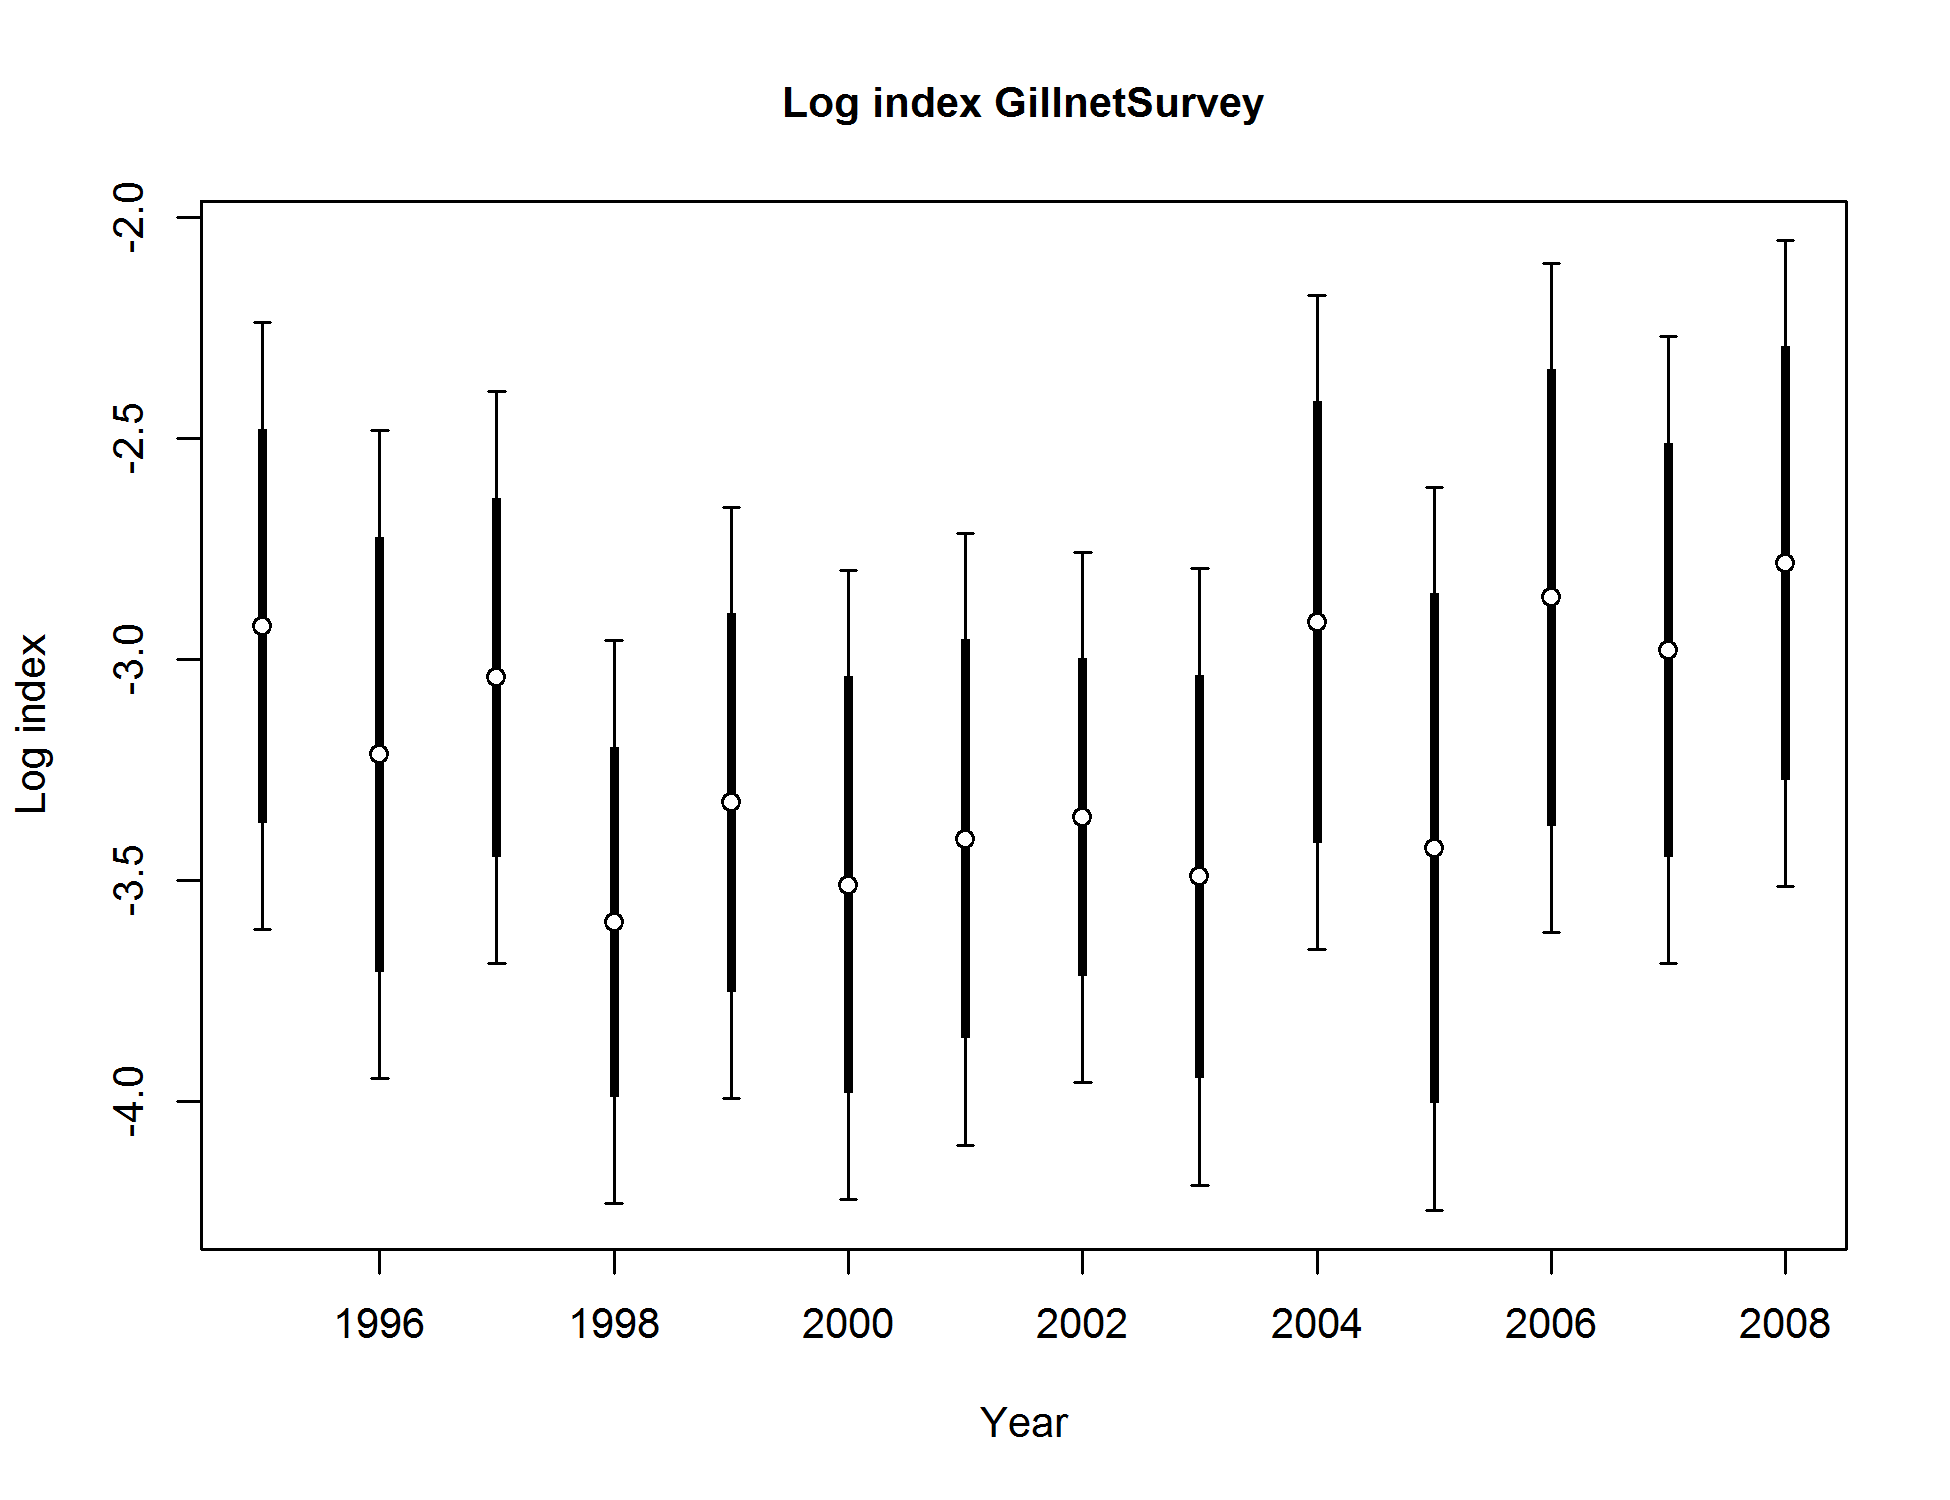
\includegraphics{r4ss/plots_mod1/index4_logcpuedata_GillnetSurvey.png}

\end{frame}

\begin{frame}{Southern California Bight Trawl Survey Index}

\textbf{Sample}: Bight Trawl Survey \textbf{Years}: 1994, 1998, 2003,
2008, 2013 \textbf{Effort}: Tow time

\includegraphics[height=7cm]{Figures/Fleet11_SCBSurvey_map.pdf}

\end{frame}

\begin{frame}{Southern California Bight Trawl Survey Index}

\begincols
 \begincol{.6\textwidth}

\begin{table}[ht]
\centering
\scalebox{0.5}{
\begin{tabular}{p{.8in}p{2in}p{.6in}p{.6in}}
  \hline
Filter & Criteria & Pos. trips & Trips \\ 
  \hline
All trawls & No filter & 158 & 944 \\ 
  Depth & Trawls $<$ 98 m (retains 95\% of all data) & 149 & 662 \\ 
  Region & Exclude trawls in harbors, north of Ventura and islands (few scorpionfish) & 129 & \textbf{398} \\ 
   \hline
\end{tabular}
}
\end{table}

\begin{table}[ht]
\centering
\scalebox{0.5}{
\begin{tabular}{p{2in}p{.6in}p{.6in}}
  \hline
Model & Binomial & Lognormal \\ 
  \hline
~Year & 494.73 & 339.56 \\ 
  ~Year + Region & 490.24 & 343.16 \\ 
  ~ Year + Month & 493.02 & 336.68 \\ 
  ~ Year + Month + Region & \textbf{486.55} & \textbf{337.87} \\ 
   \hline
\end{tabular}
}
\end{table}

\endcol
 \begincol{.4\textwidth}

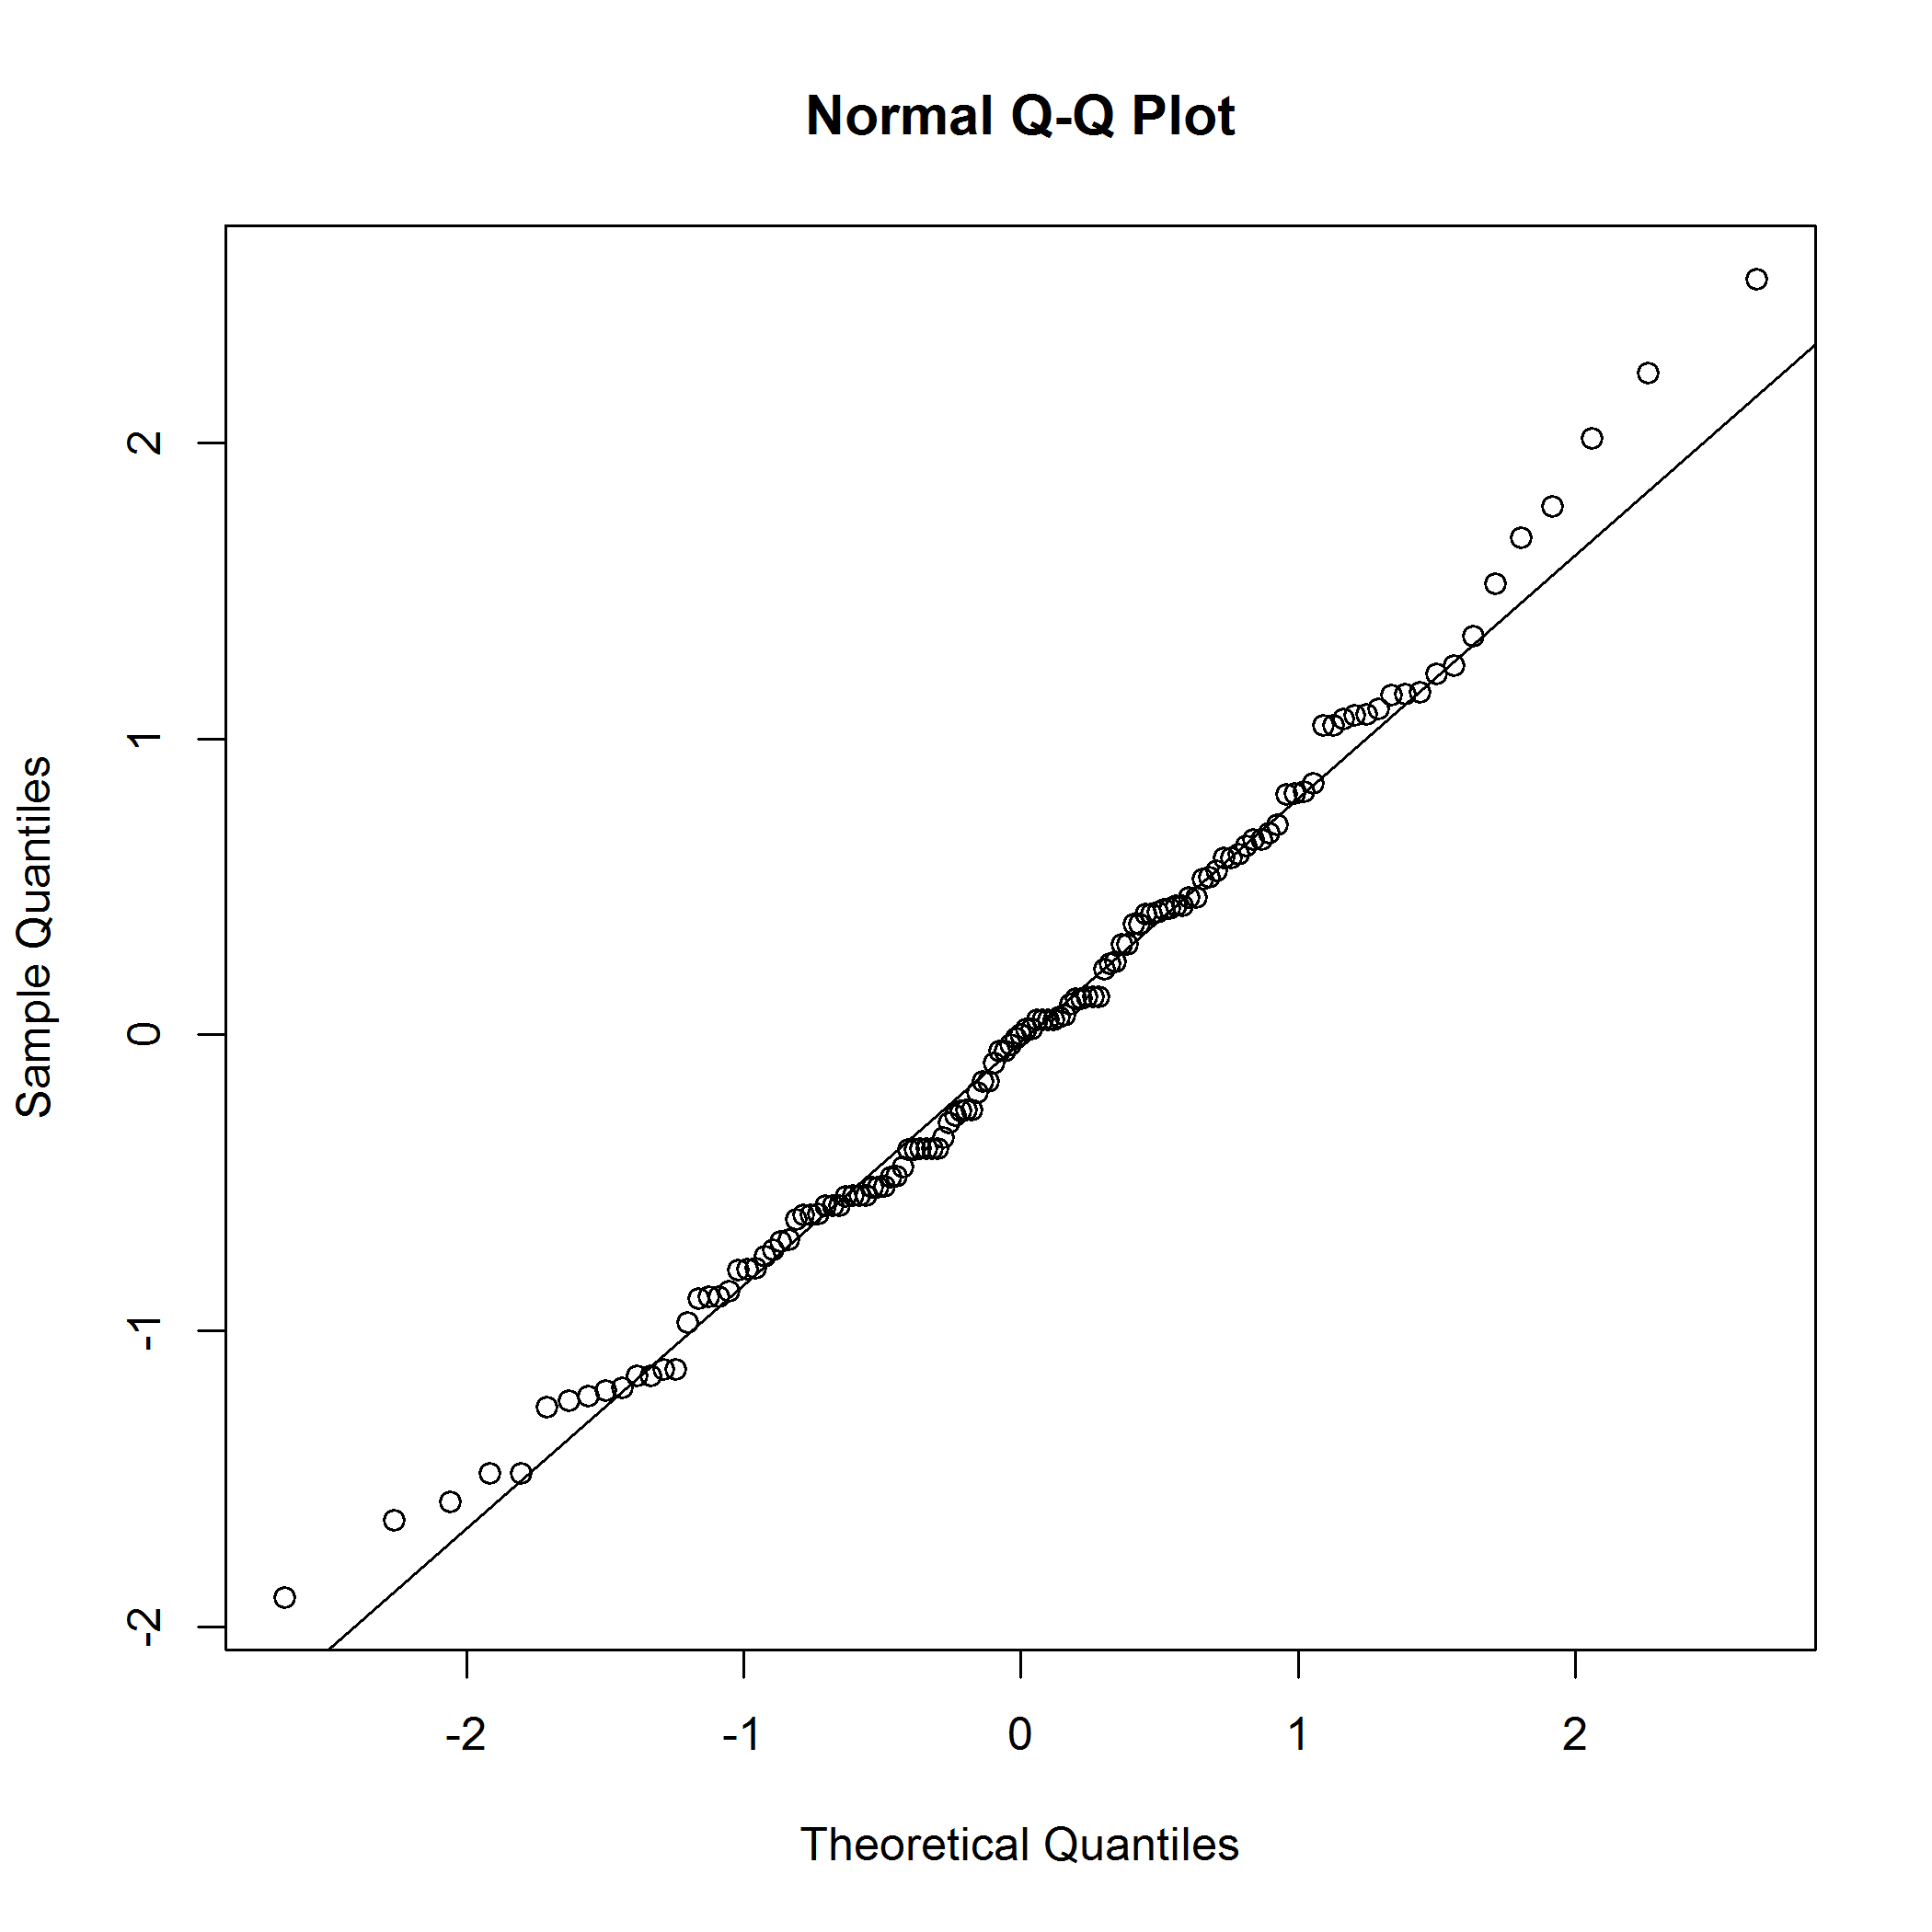
\includegraphics[height=4cm]{Figures/Fleet11_SCBsurvey_QQ.png} \endcol
\endcols

\end{frame}

\begin{frame}{Southern California Bight Trawl Survey Index}

\textbf{Results}\\
\centering
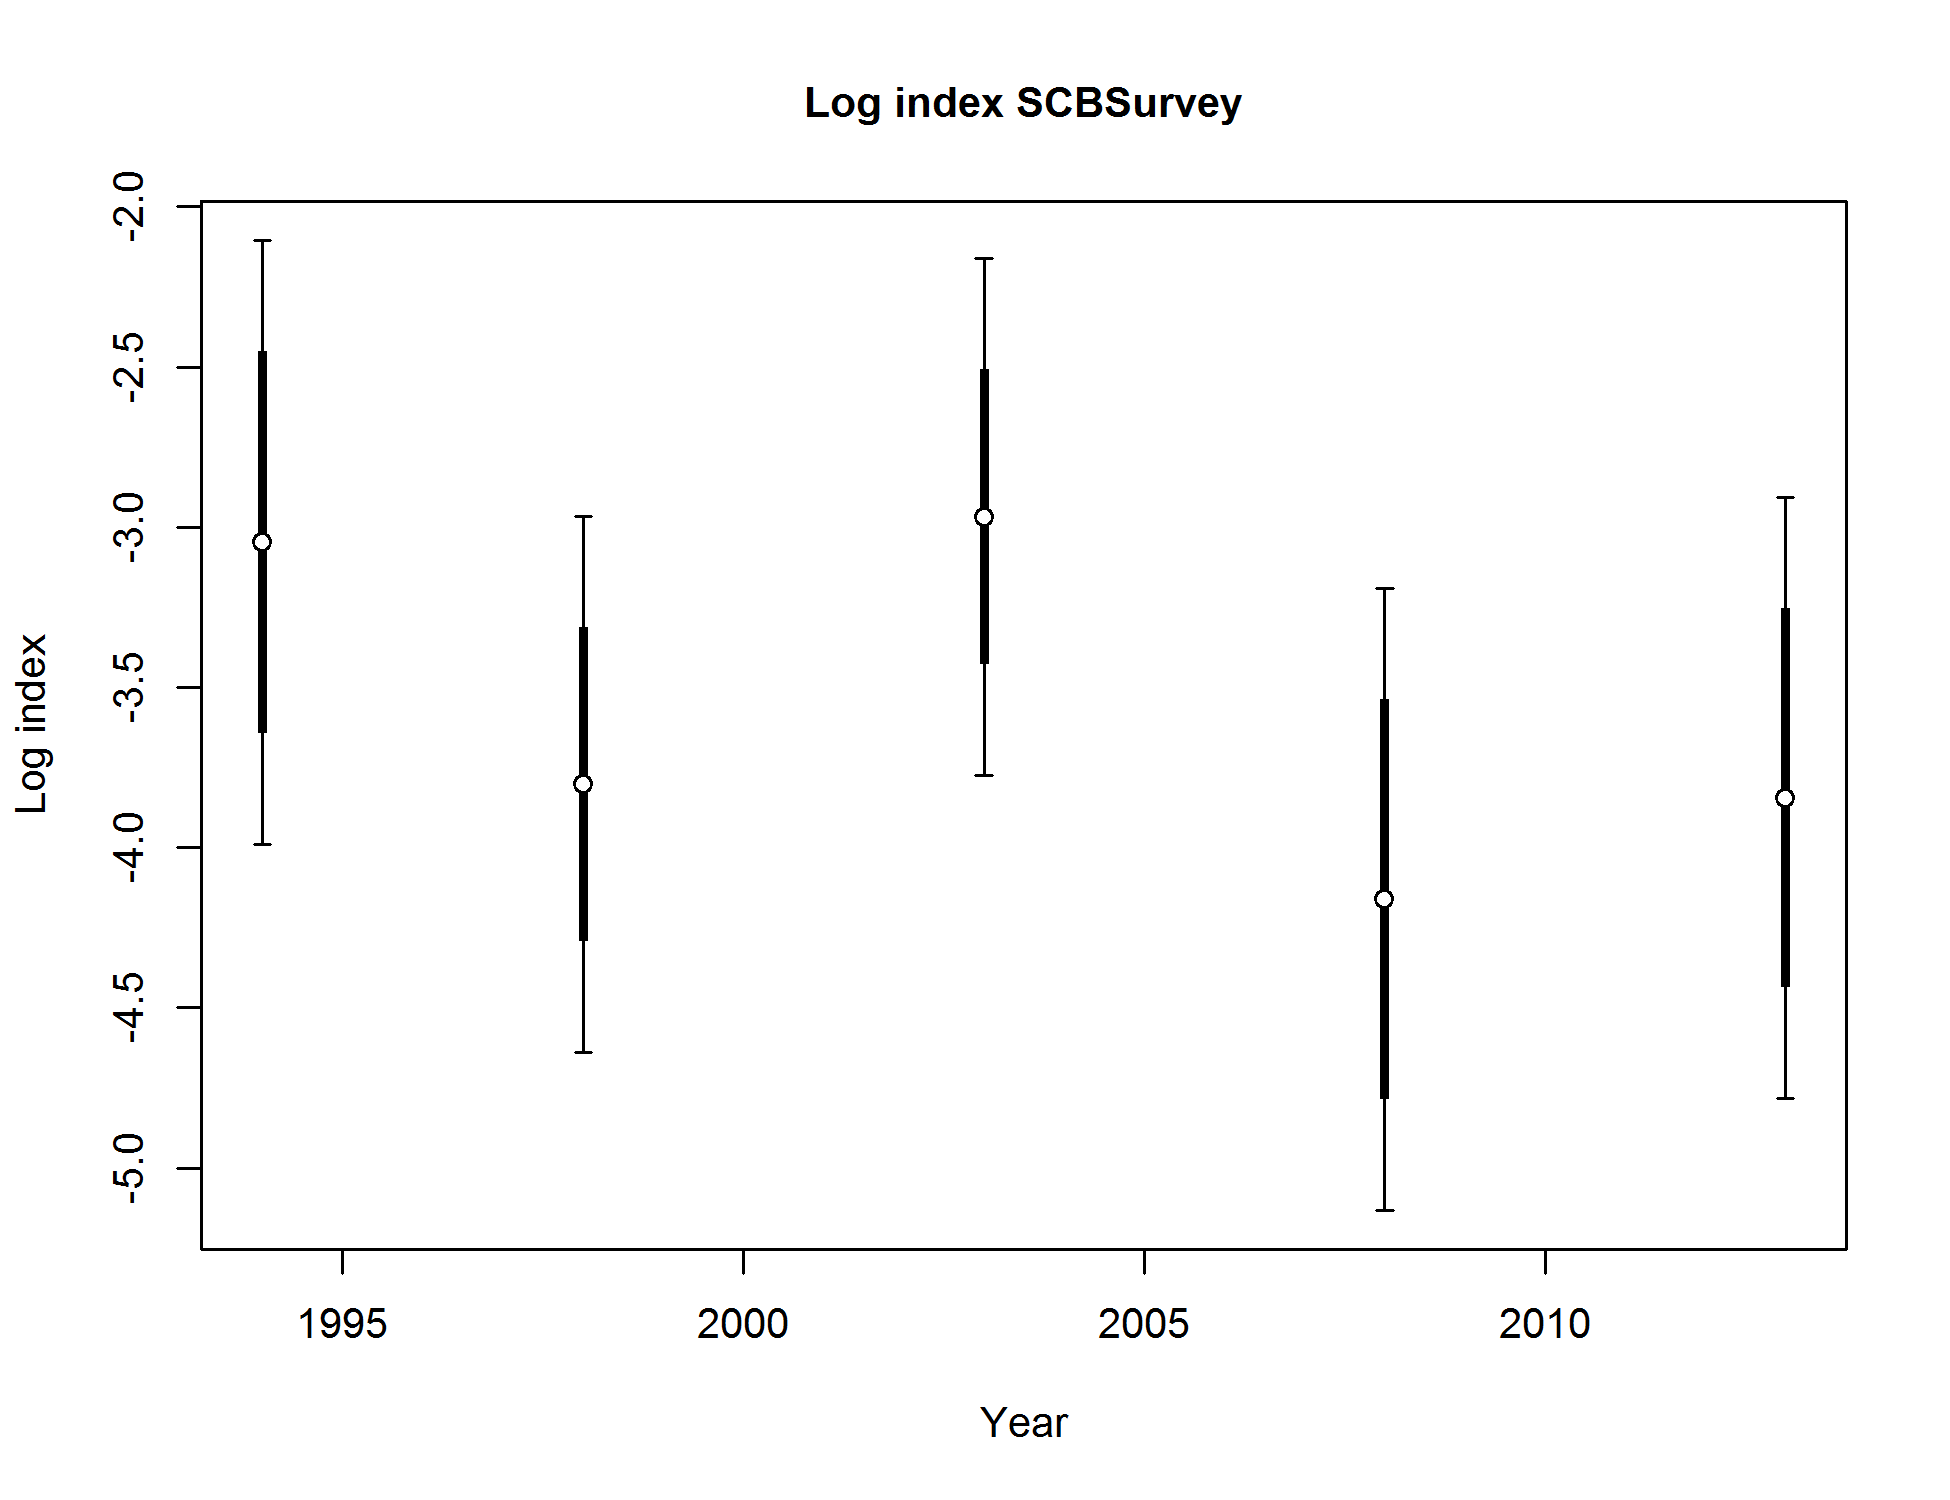
\includegraphics{r4ss/plots_mod1/index4_logcpuedata_SCBSurvey.png}

\end{frame}

\begin{frame}{NWFSC Trawl Survey Index}

Geostatistical approach Vector Autoregressive Spatio-Temporal (VAST)
model

\begin{itemize}
\item[$\bullet$] Uses delta-GLMM framework
\begin{itemize}
\item[$\circ$] Probability of encounters
\item[$\circ$] Catch rates for non-zero catches
\end{itemize}
\item[$\bullet$] Geostatistical approach
\begin{itemize}
\item[$\circ$] Divides survey area into fine-scale grids
\item[$\circ$] Assumes that nearby grids have more similar fish density than those further away
\item[$\circ$] Smooths density estimates over the landscape
\item[$\circ$] Reduces uncertainty in the estimates
\end{itemize}
\end{itemize}

\end{frame}

\begin{frame}{NWFSC Trawl Survey Index}

\textbf{Sample}: California MRFSS and CRFS \textbf{Years}: 1980-2003
\textbf{Effort}: Angler hours

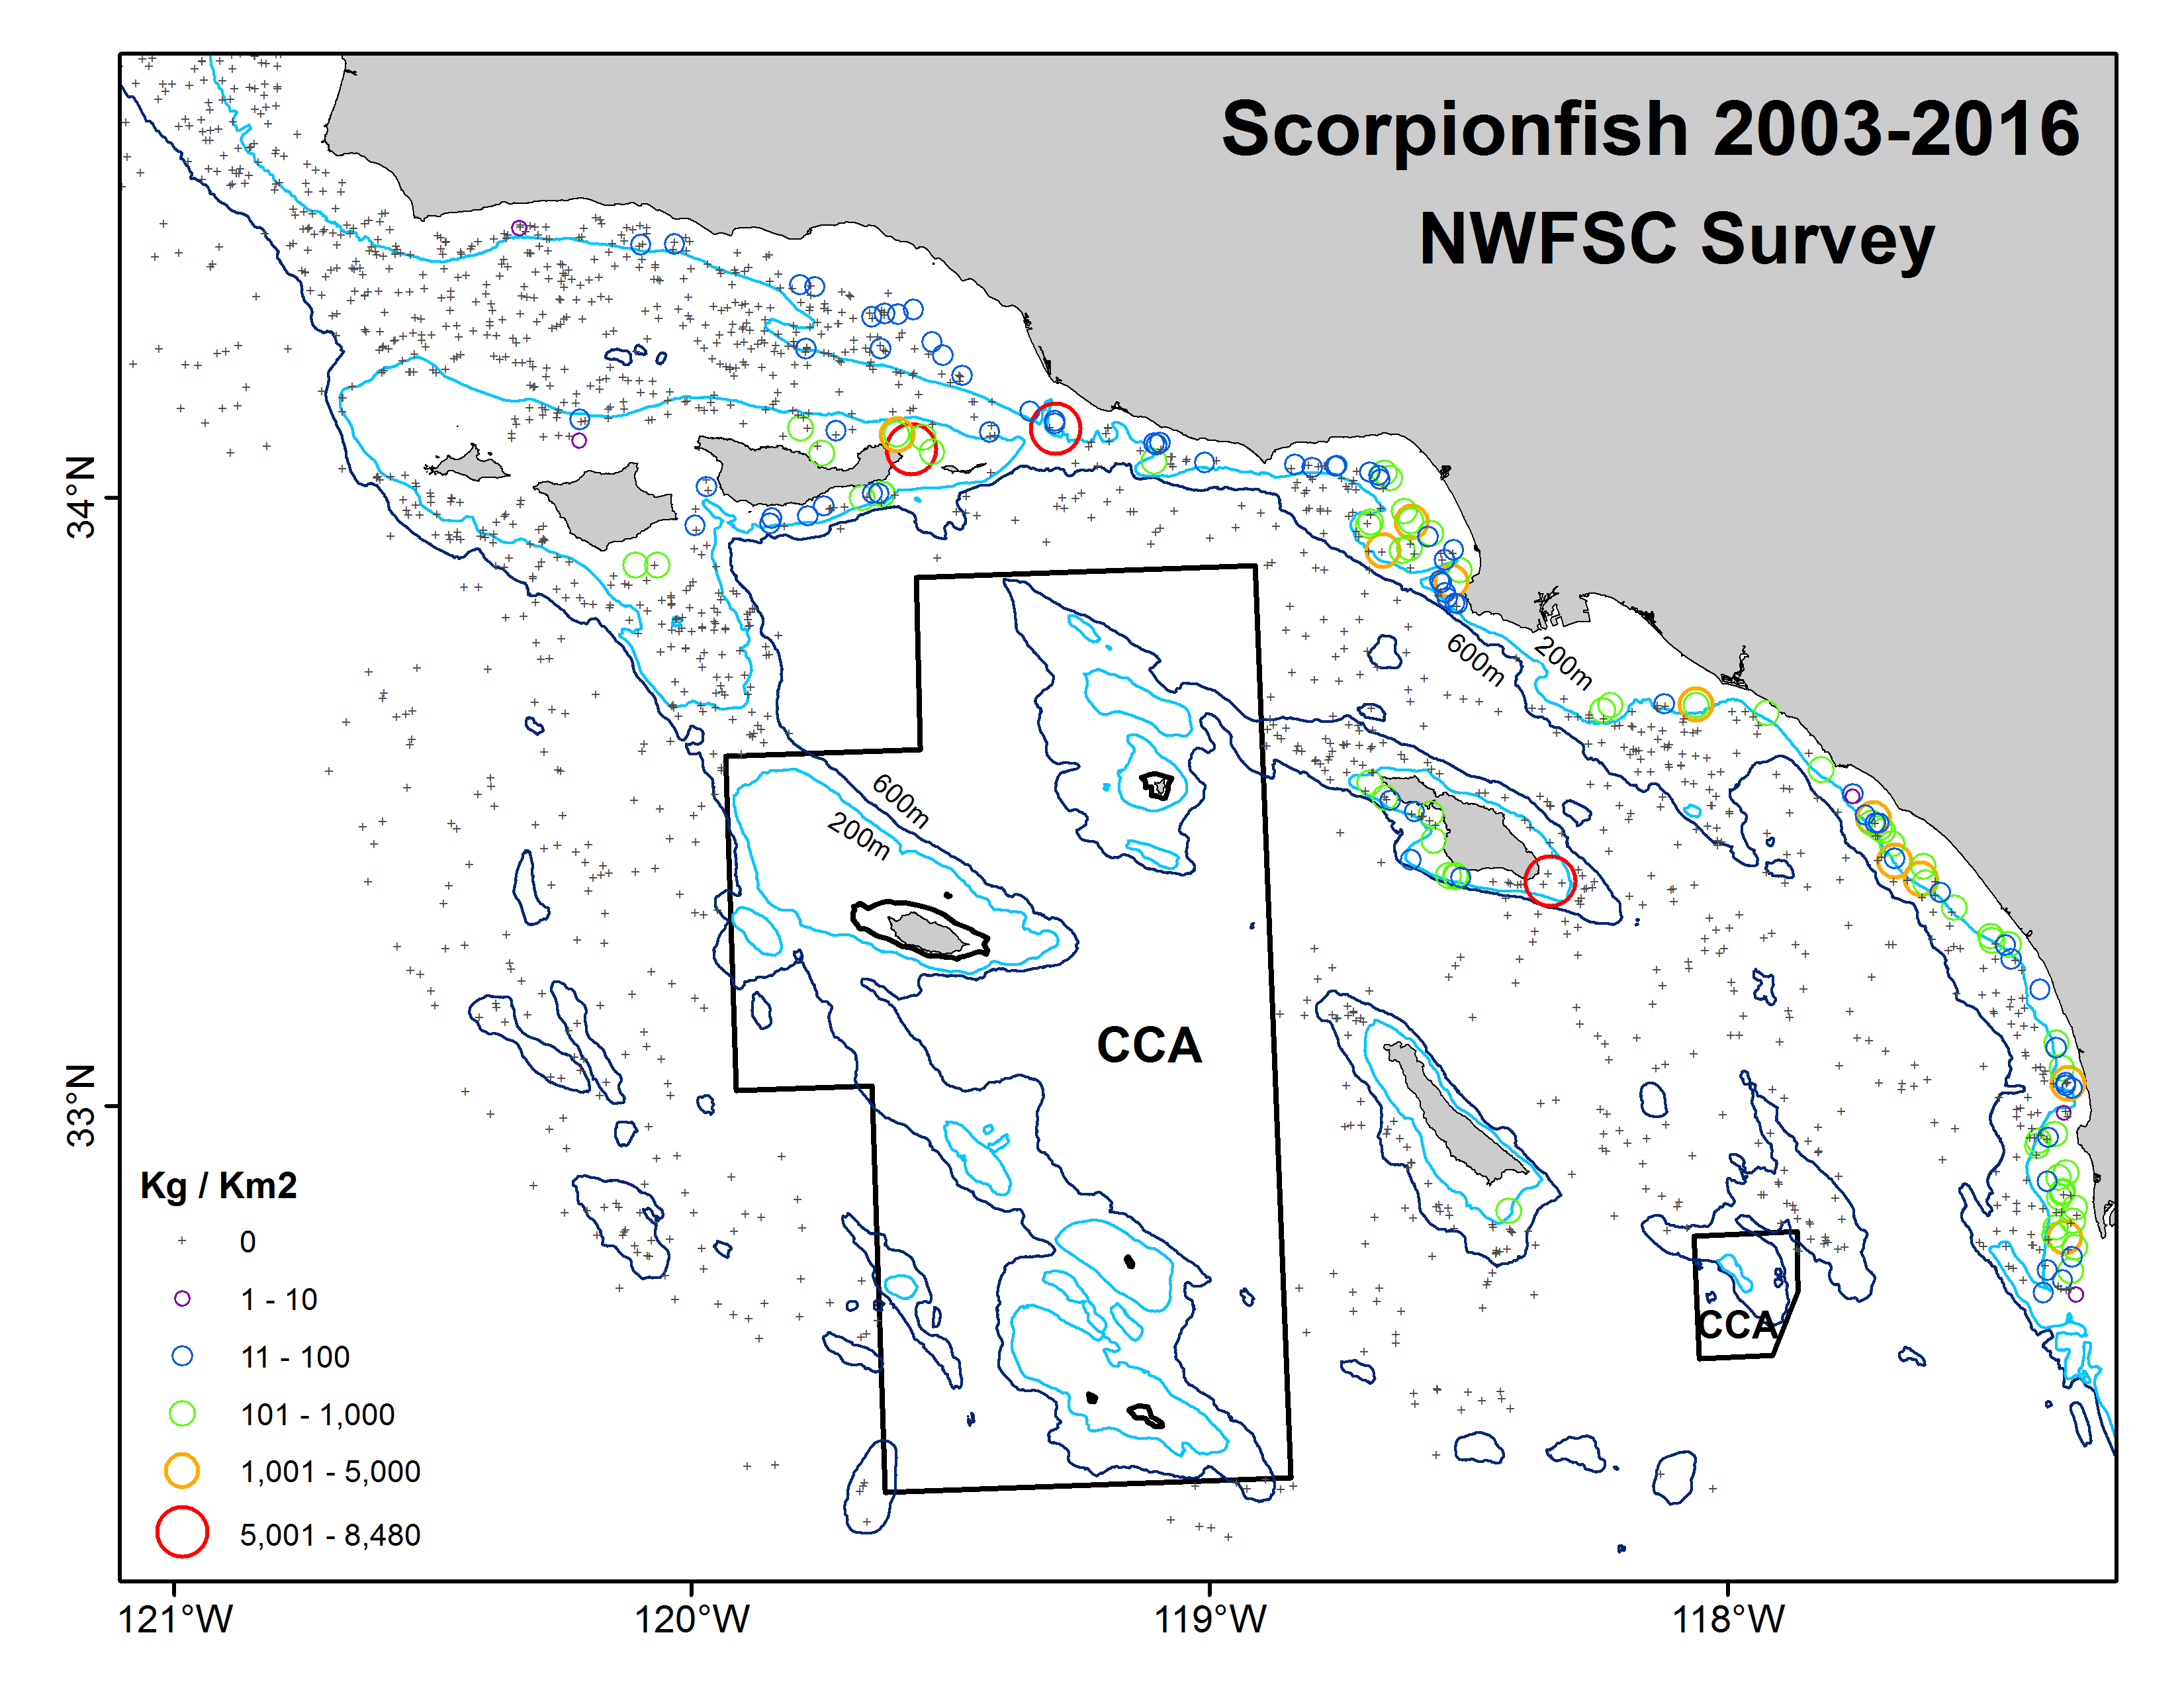
\includegraphics[height=.7\textheight]{Figures/NWFSCtrawl_map.png}

\end{frame}

\begin{frame}{NWFSC Trawl Survey Index}

Proportion of positive tows and raw catch rate by depth (left) and
latitude (right) \begincols
 \begincol{.5\textwidth} \centering
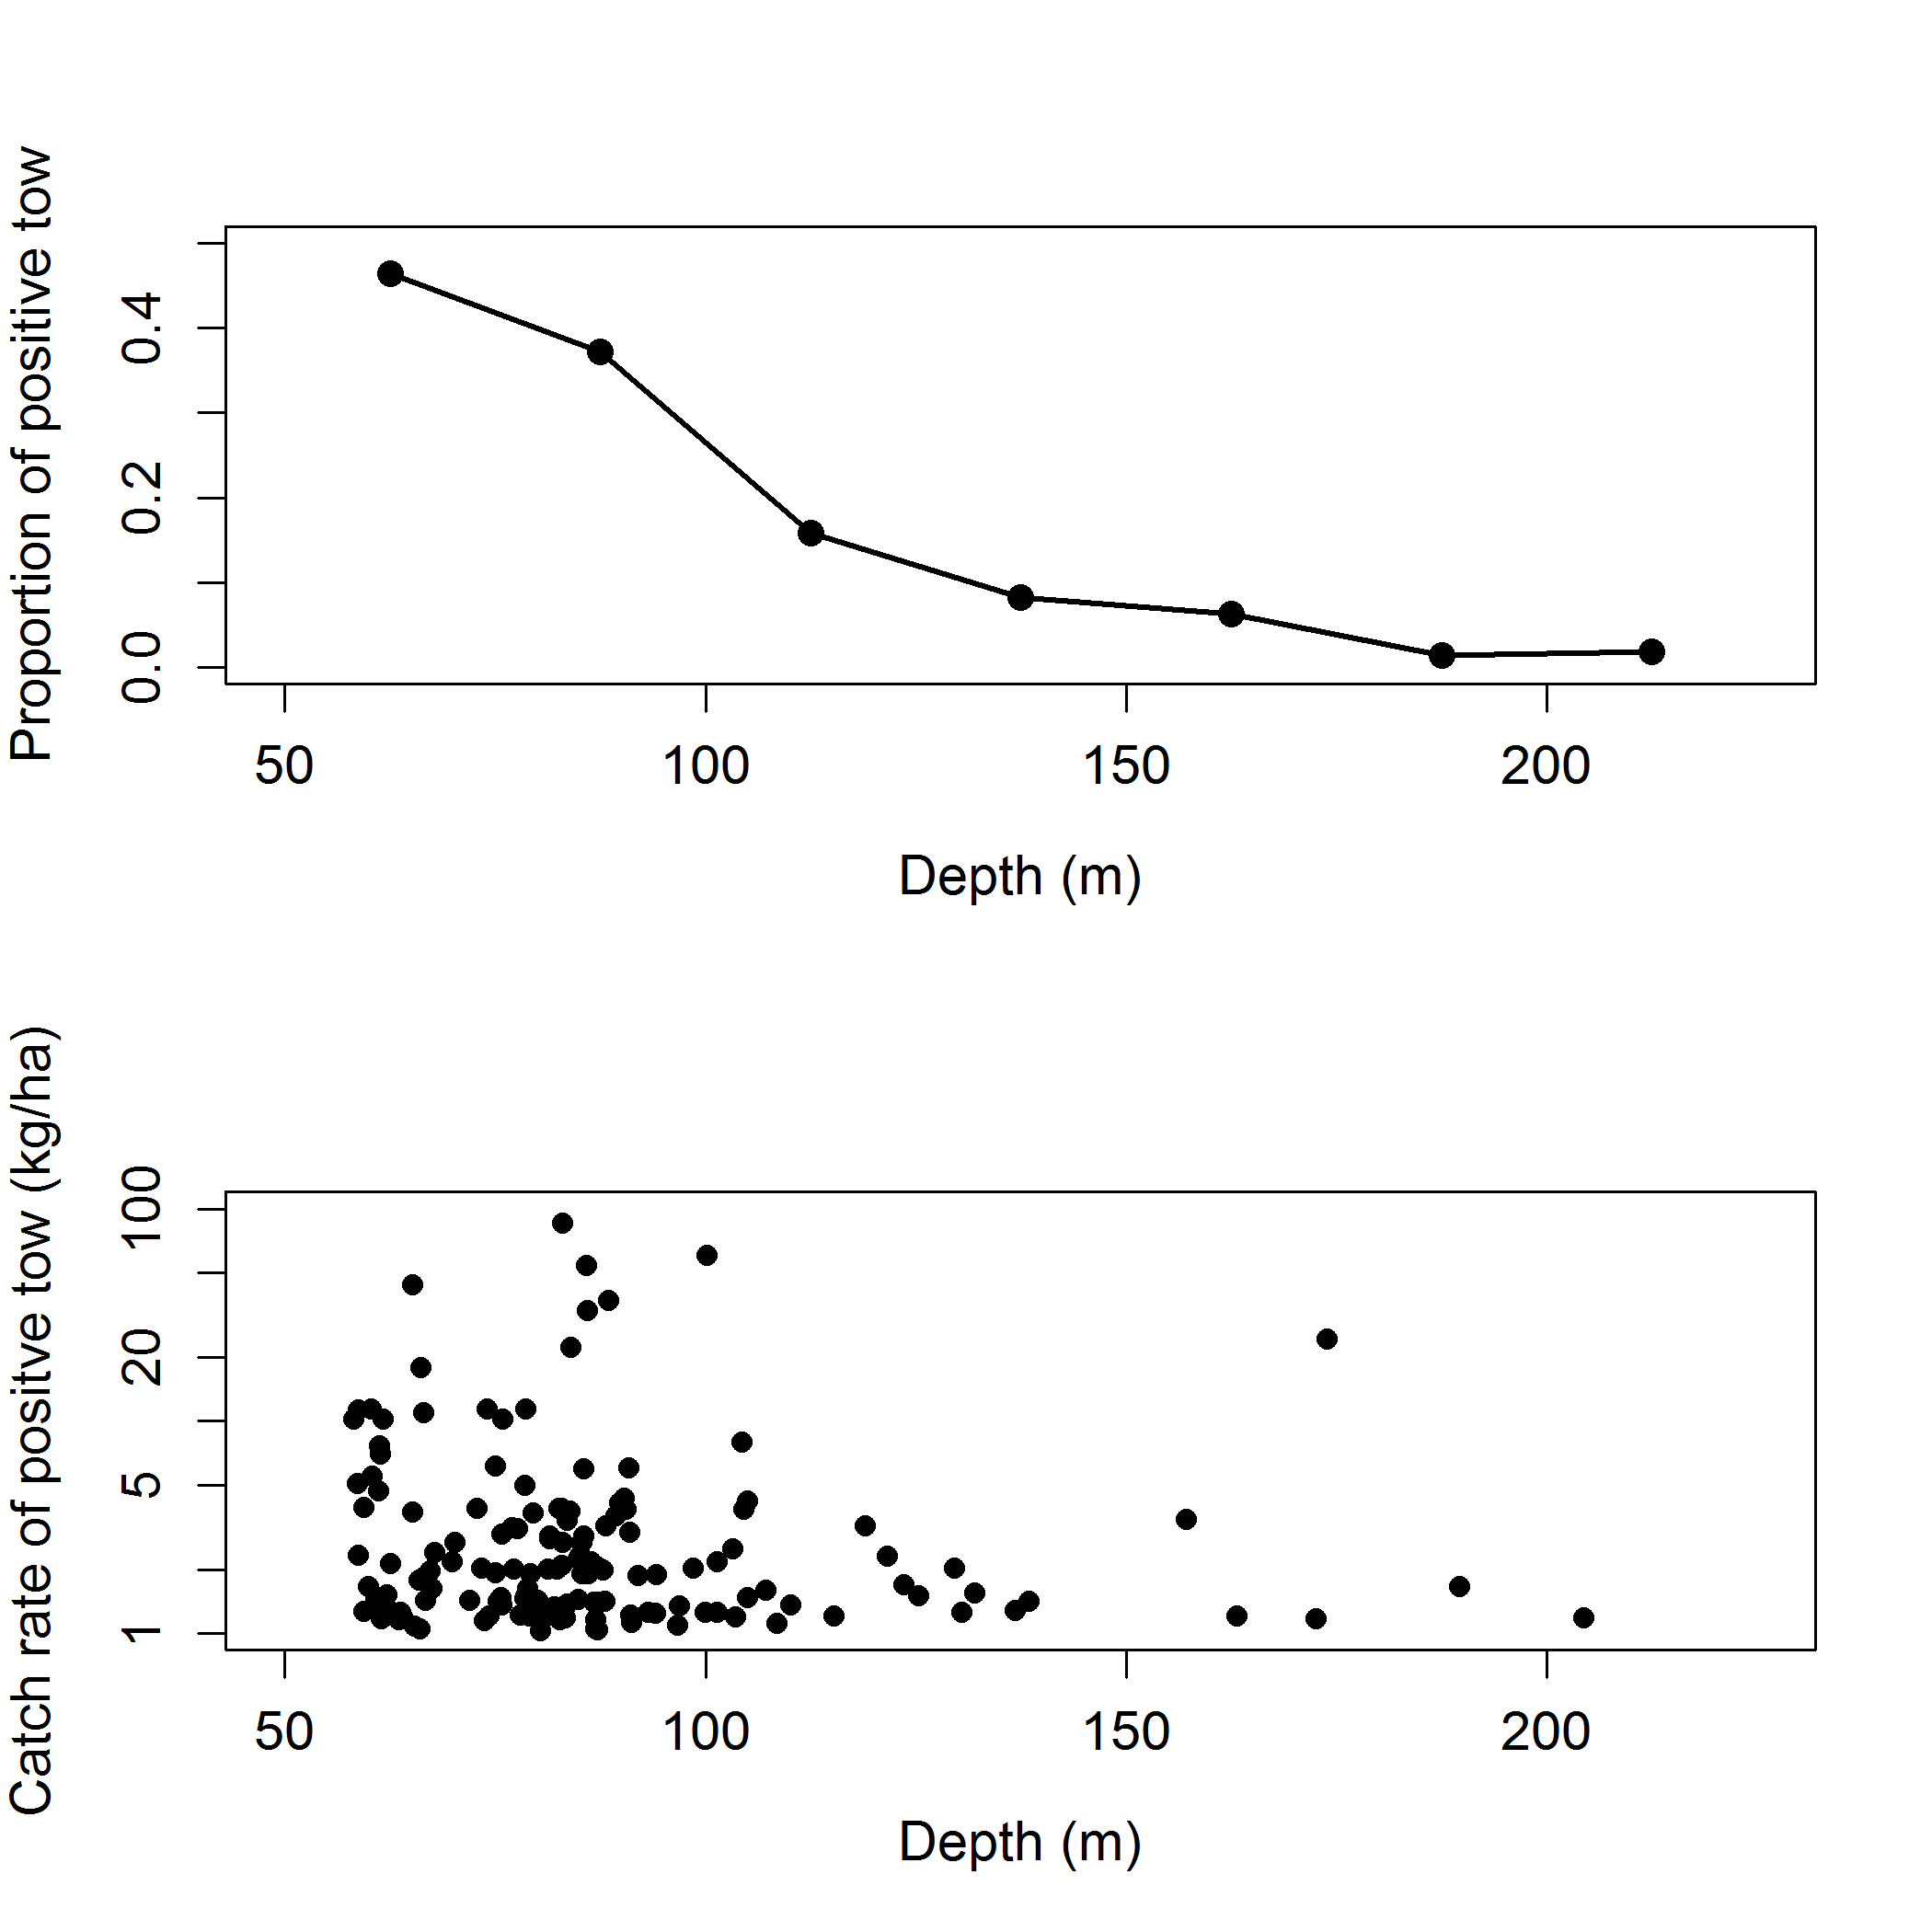
\includegraphics{Figures/NWFSCtrawl_posdepth.png}

\endcol
 \begincol{.5\textwidth}

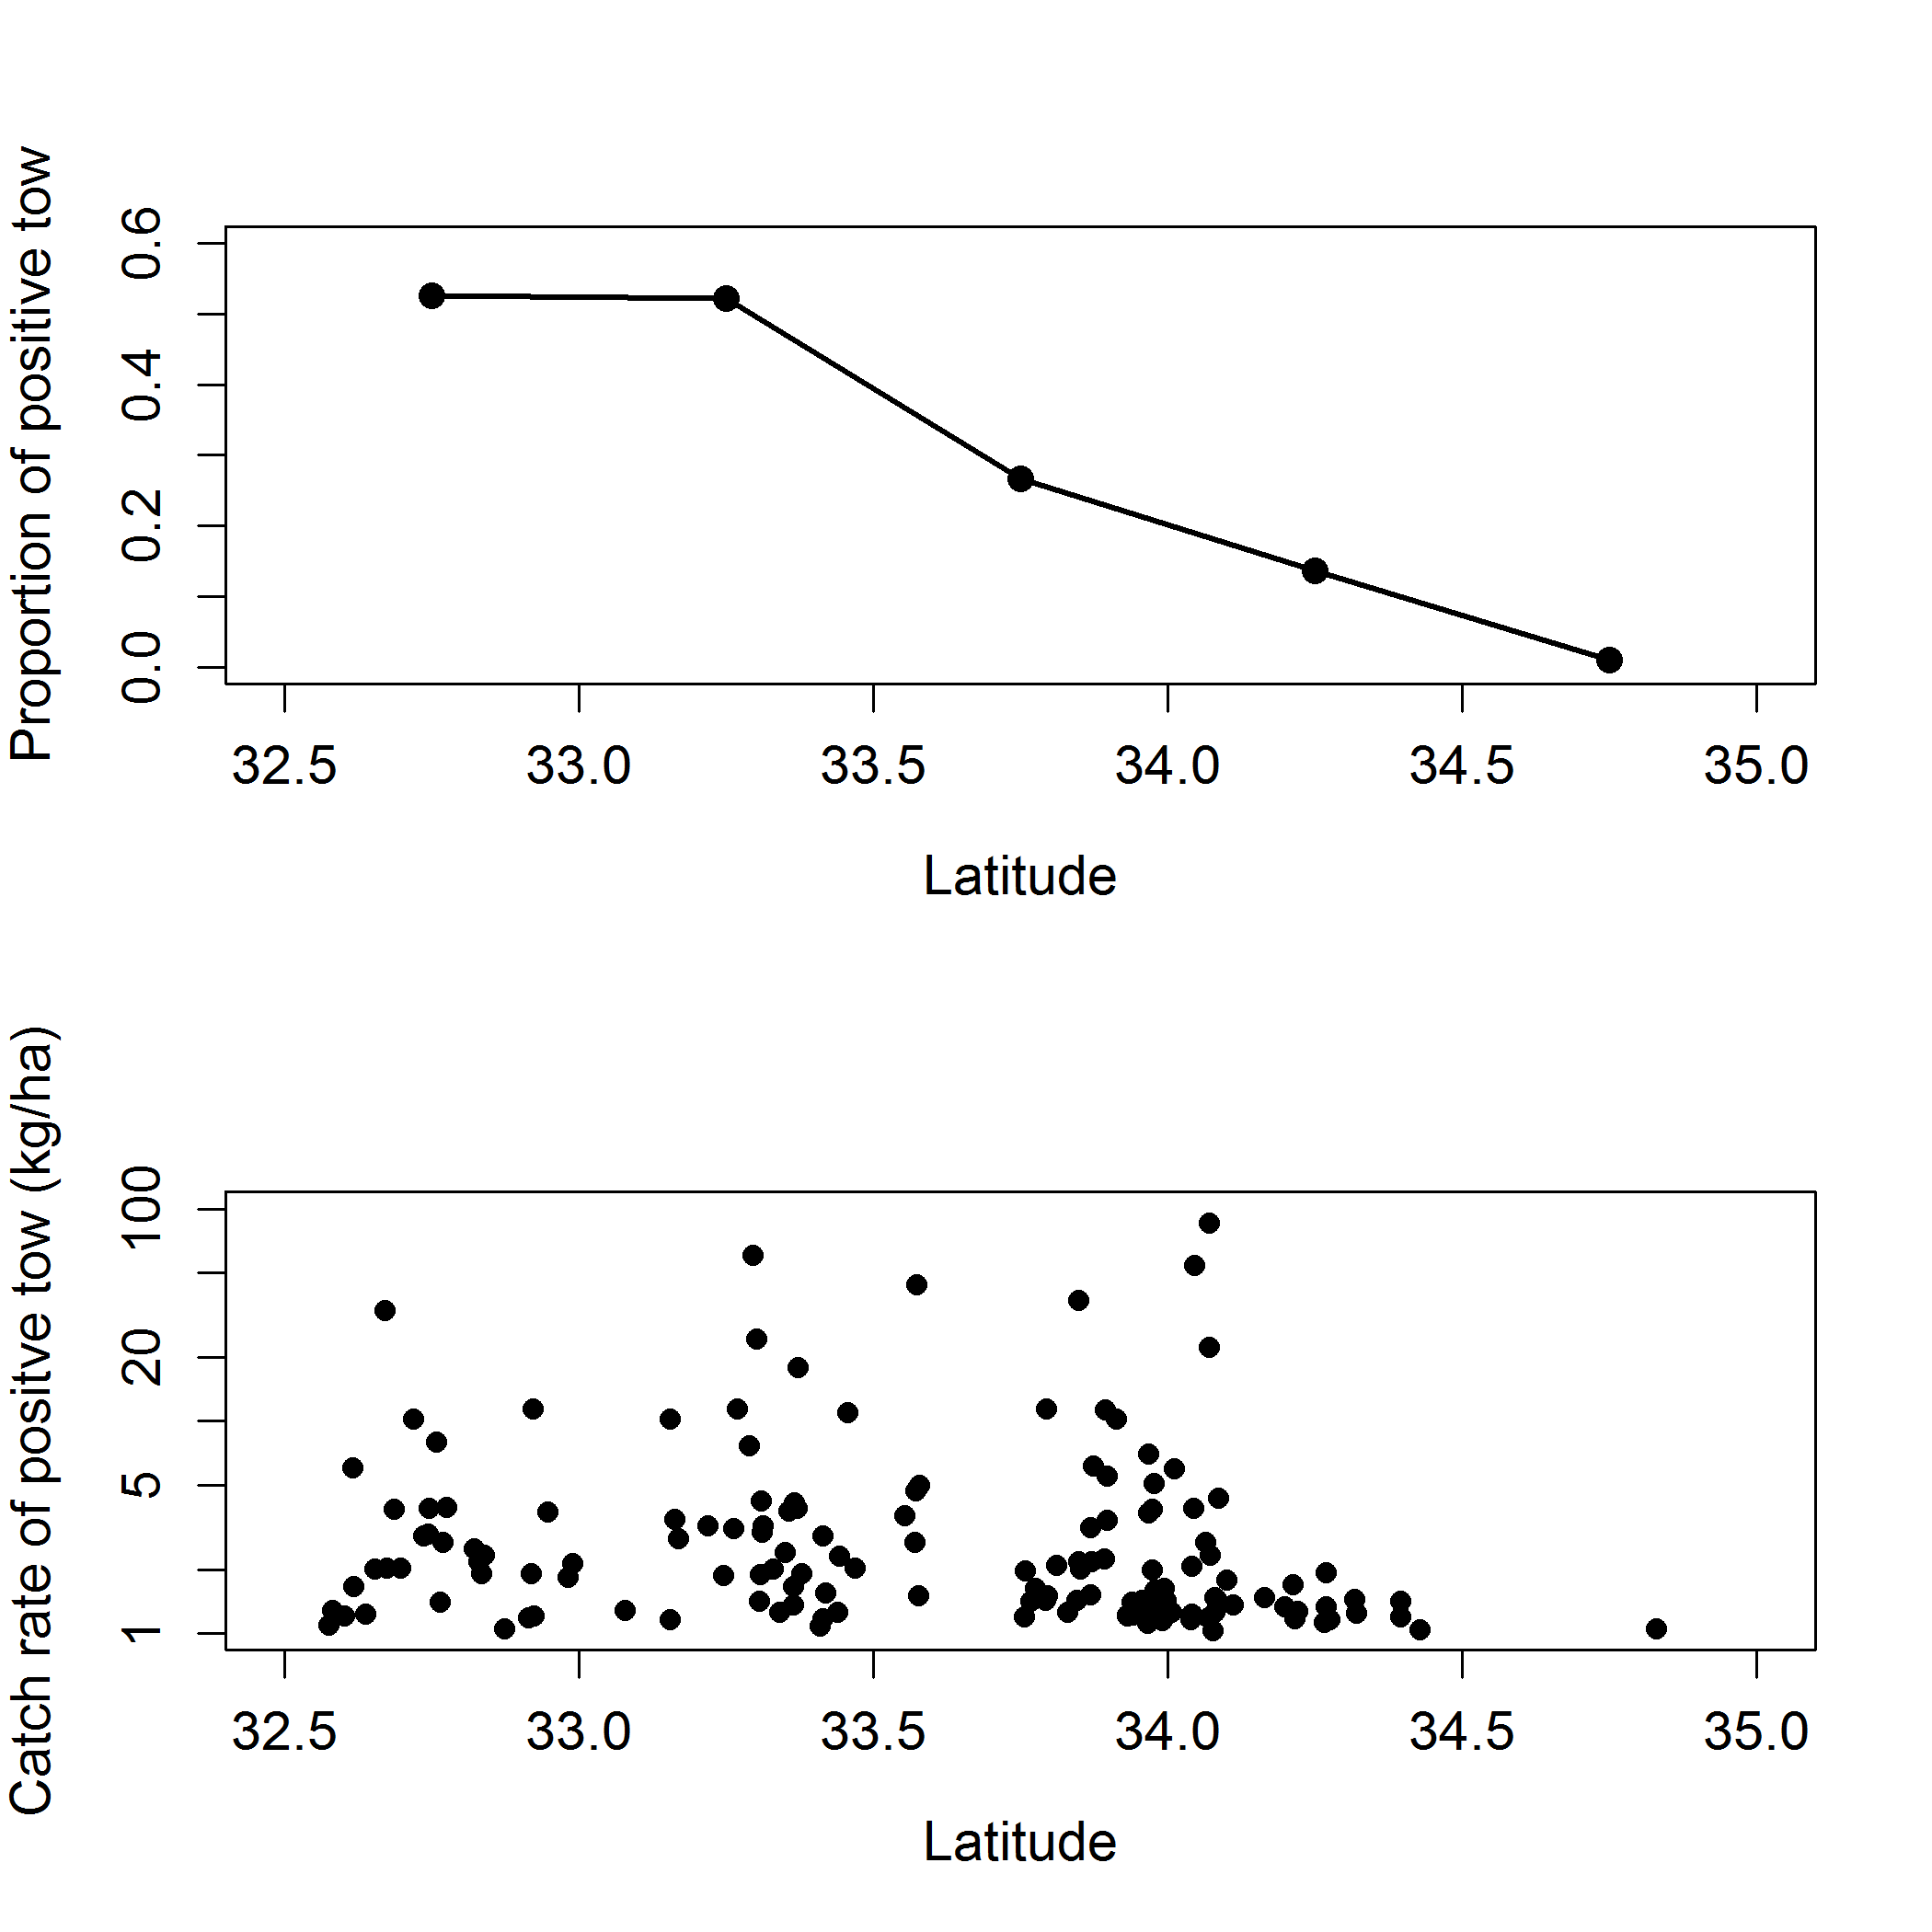
\includegraphics{Figures/NWFSCtrawl_poslat.png}

\endcol
\endcols

\end{frame}

\begin{frame}{NWFSC Trawl Survey Index}

Comparison of length data by sex and depth (left) and latitude (right)
\begincols
 \begincol{.5\textwidth}
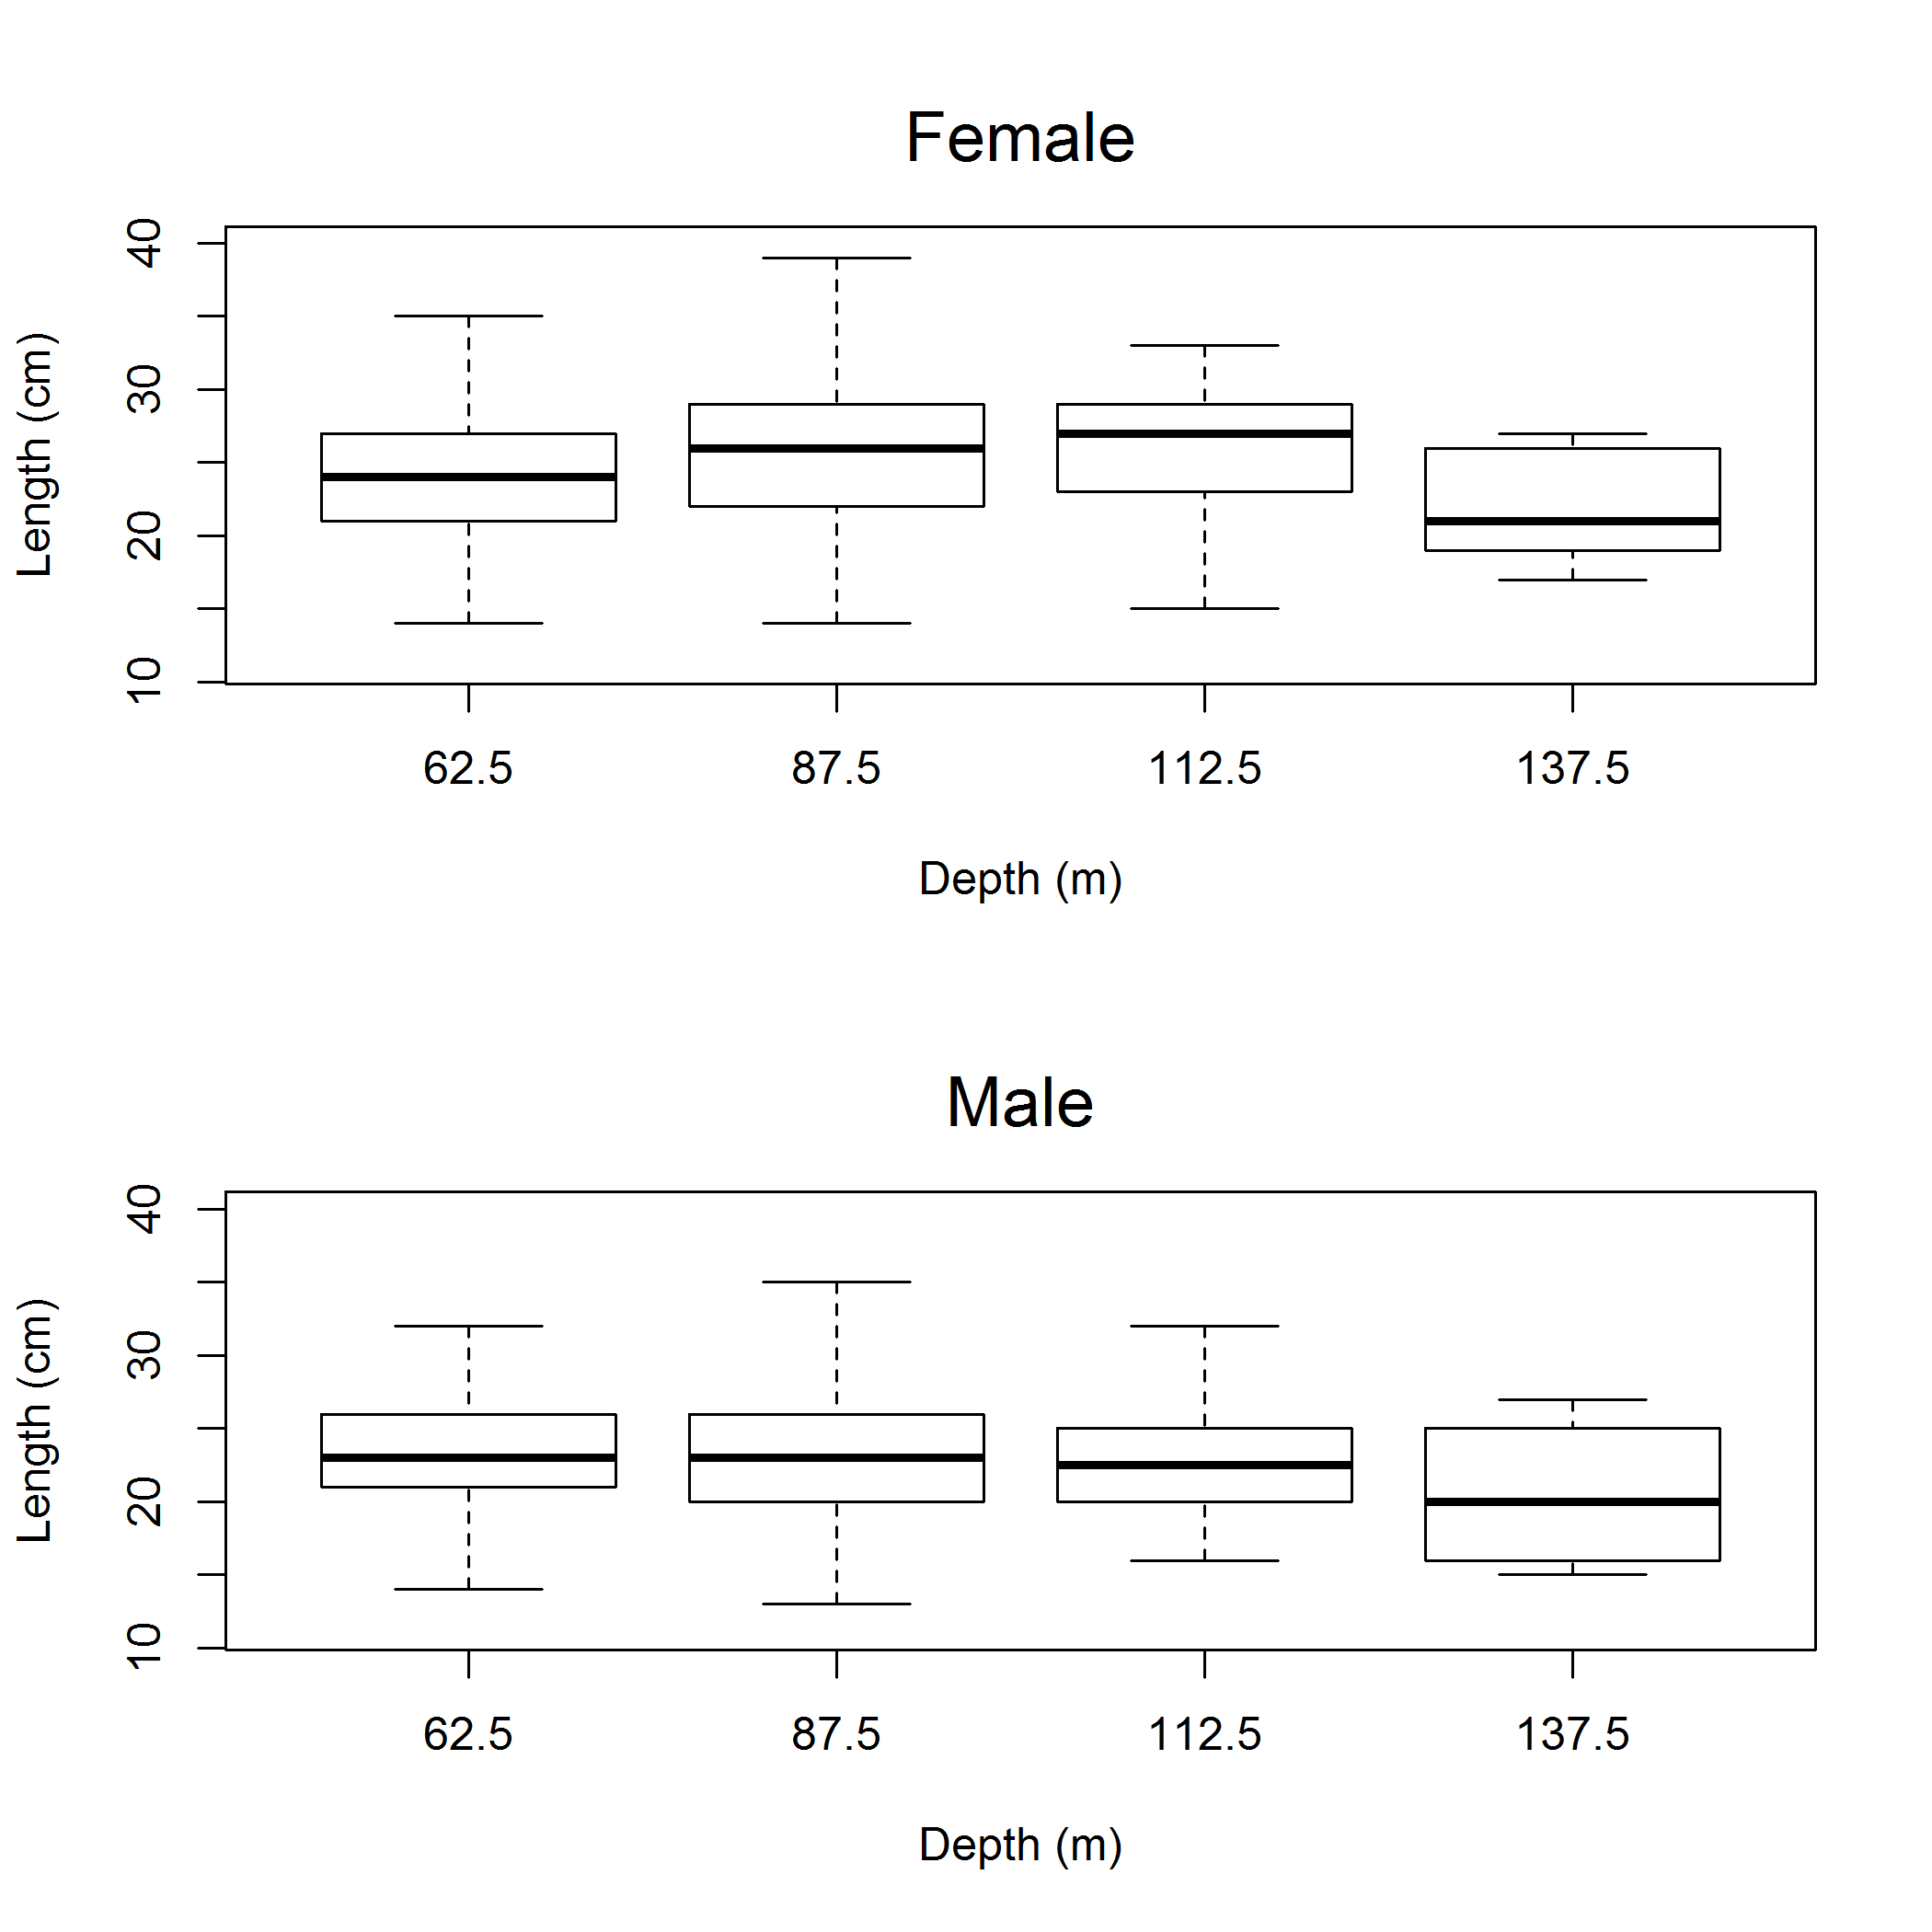
\includegraphics{Figures/NWFSCtrawl_lengthdepth.png}

\endcol
 \begincol{.5\textwidth}

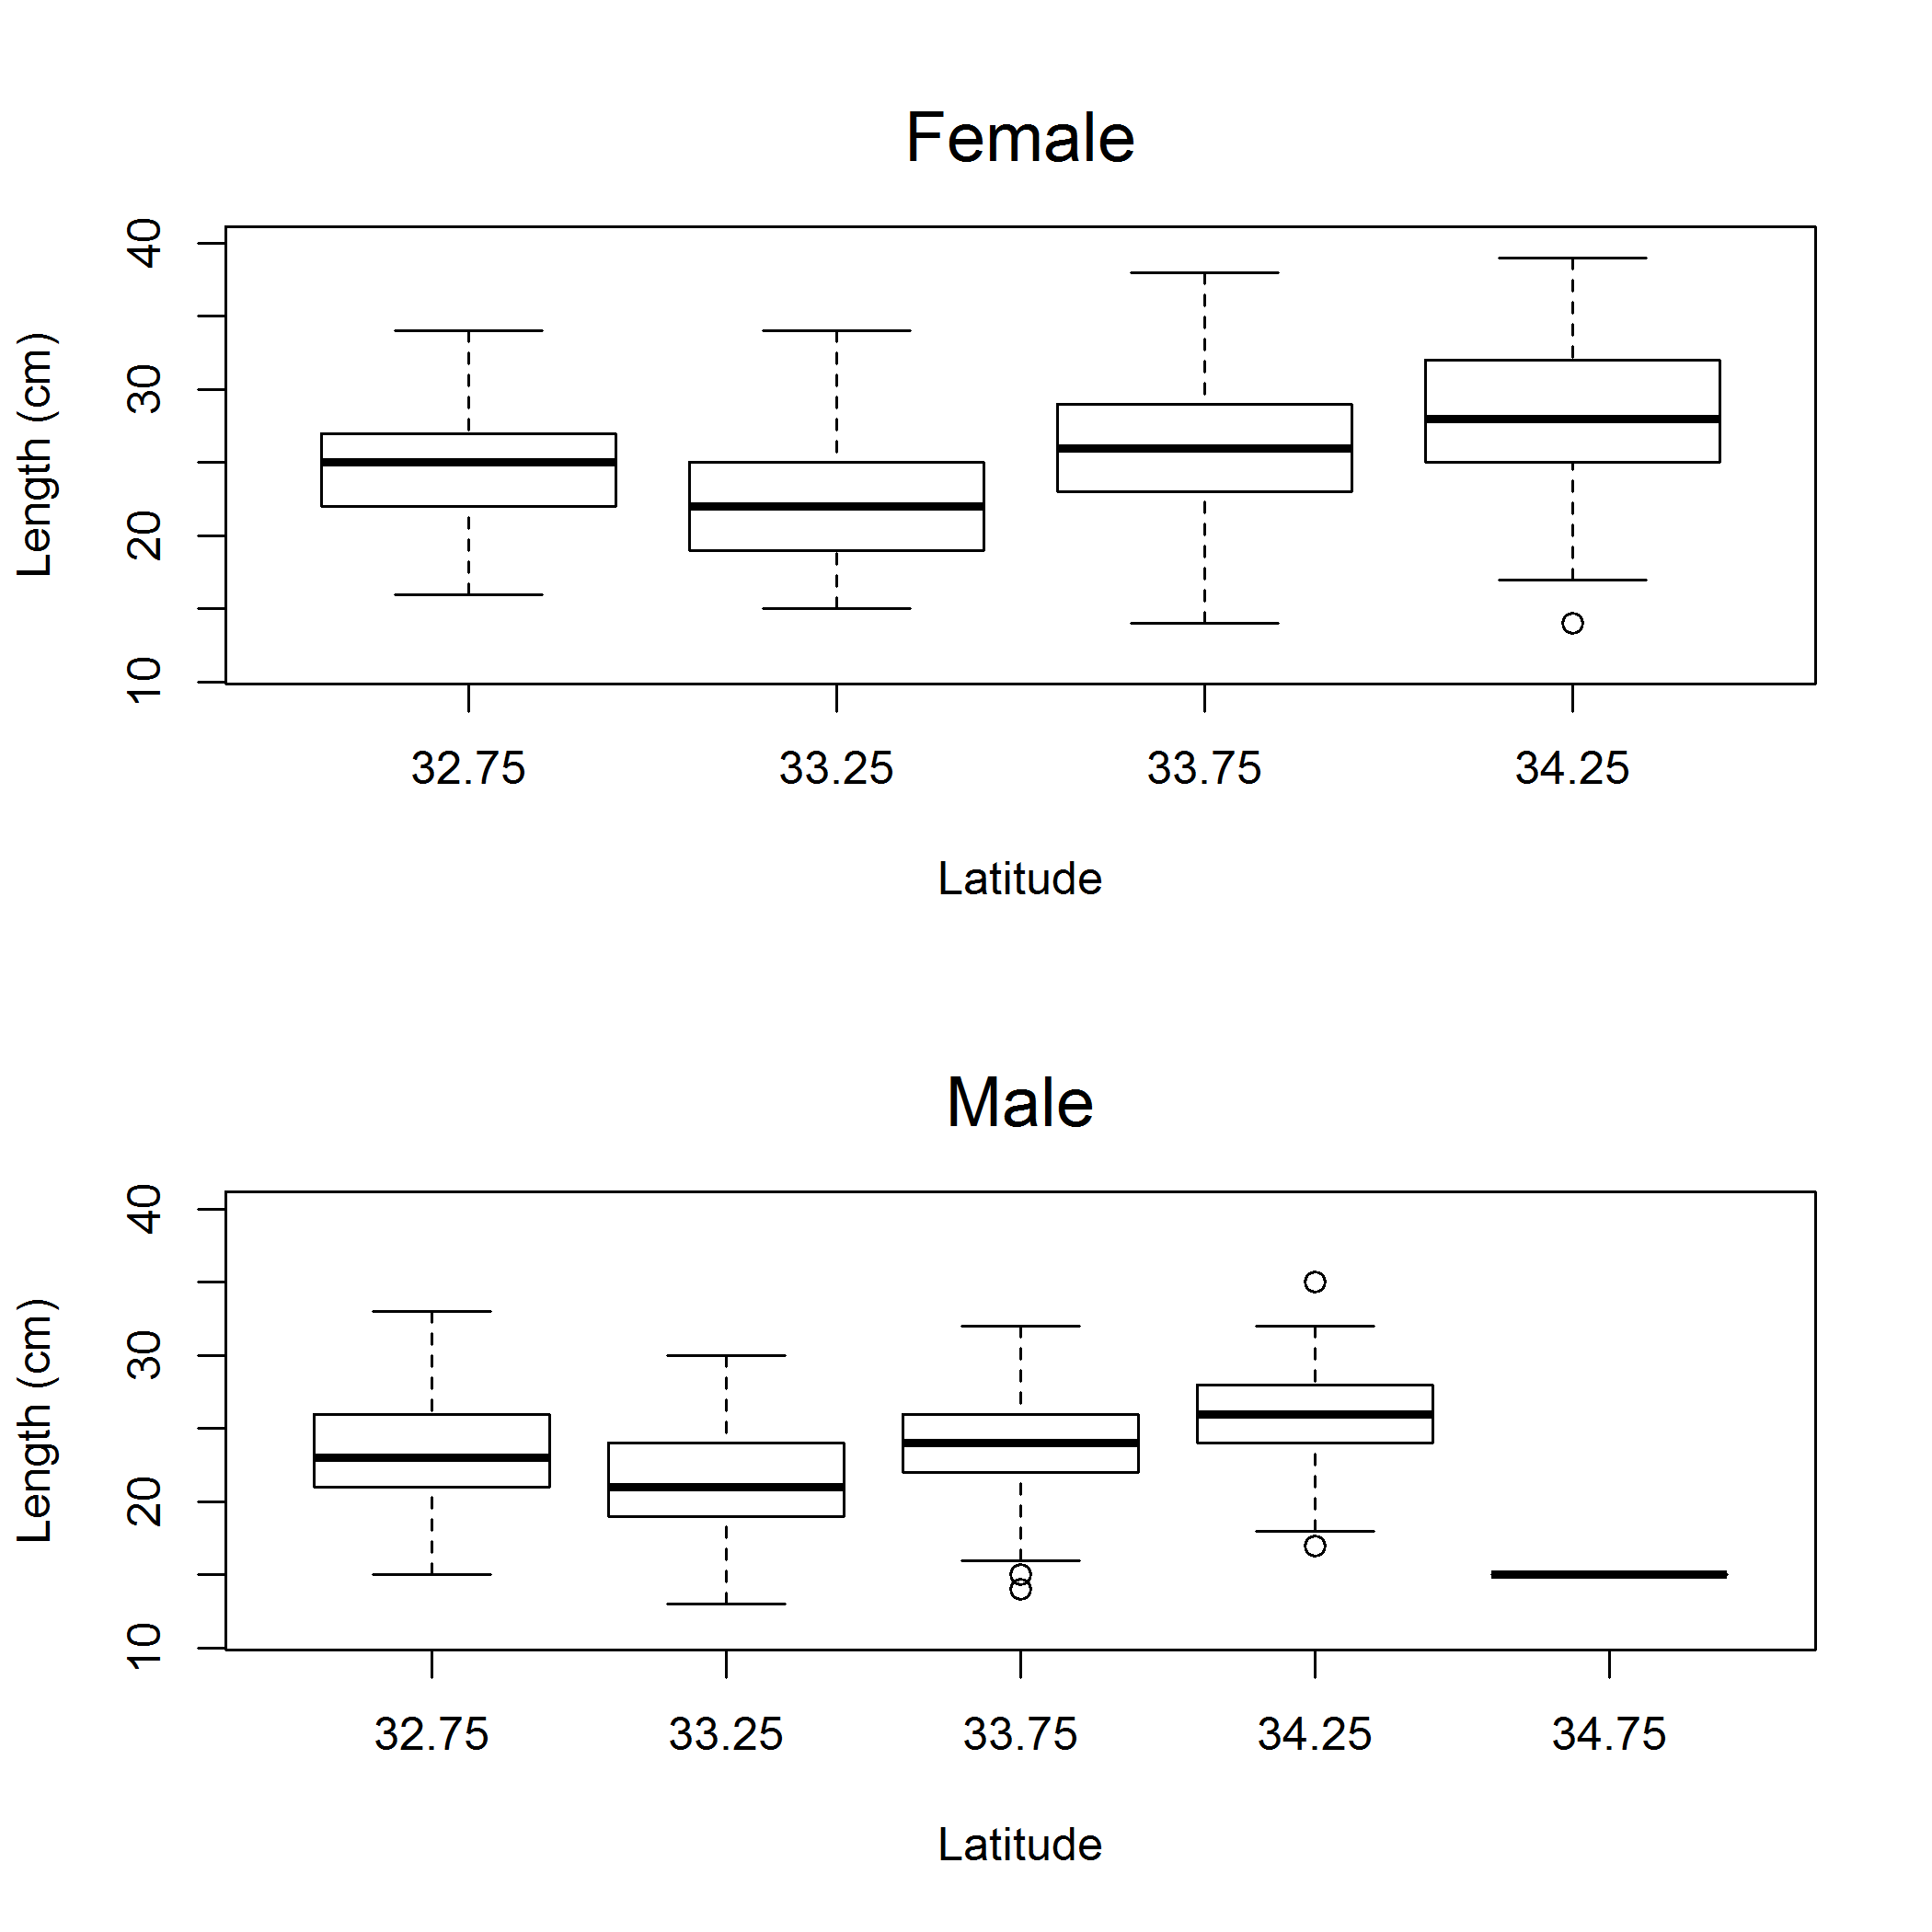
\includegraphics{Figures/NWFSCtrawl_lengthlat.png}

\endcol
\endcols

\end{frame}

\begin{frame}{NWFSC Trawl Survey Index}

\begincols
 \begincol{.5\textwidth}
\includegraphics[height=4cm]{Figures/Fleet8_NWFSCtrawl_CompareVAST.png}
\endcol
 \begincol{.5\textwidth}
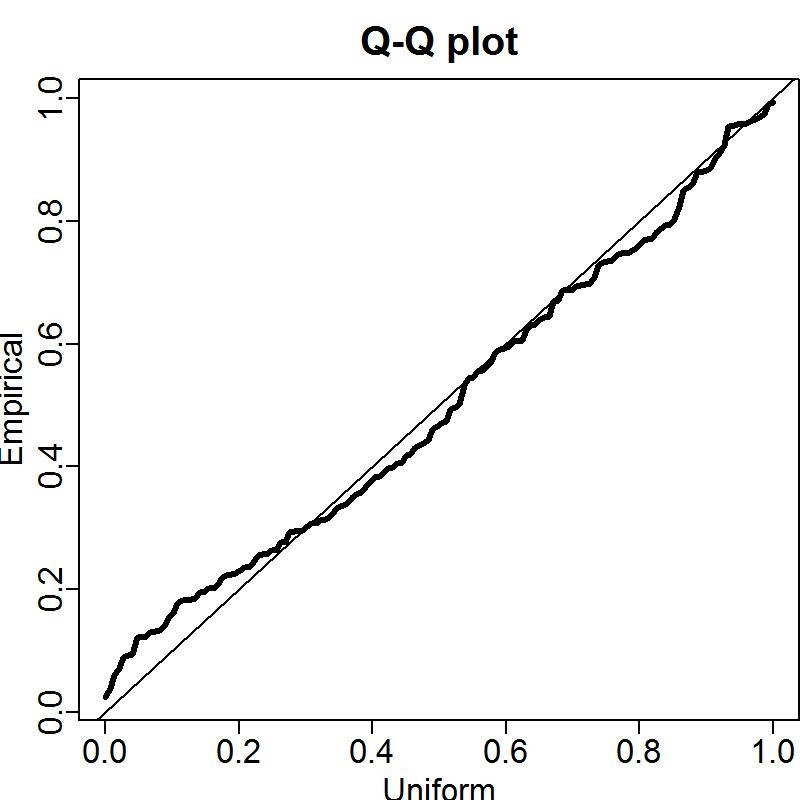
\includegraphics[height=4cm]{Figures/NWFSCtrawl_QQ.jpg}

\endcol
\endcols

\end{frame}

\begin{frame}{NWFSC Trawl Survey Index}

\textbf{Comparison with the GLMM}

\end{frame}

\begin{frame}{NWFSC Trawl Survey Index}

\centering
\includegraphics{r4ss/plots_mod1/index4_logcpuedata_NWFSCtrawl.png}

\end{frame}

\section{Composition}\label{composition}

\begin{frame}{Length compositions were provided from the following
sources:}

\begin{itemize}
  \item[$\bullet$] CDFW market category study (\emph{commercial dead fish}, 1996-2003)    
  \item[$\bullet$] CALCOM (\emph{commercial dead fish}, 2013-2016)    
  \item[$\bullet$] CDFW onboard observer (\emph{recreational charter discards}, 2003-2016)  
  \item[$\bullet$] Collins and Crooke onboard observer surveys (1975-1978) 
  \item[$\bullet$] Ally onboard observer study (\emph{recreational charter kept/discards}, 1984-1989)  
  \item[$\bullet$] MRFSS (1980-2003) and CRFS (2004-2014) (\emph{private and party/charter, kept})
  \item[$\bullet$] POTW trawl surveys (\emph{research}, 1970-2016)      
  \item[$\bullet$] CSUN/VRG gillnet survey (\emph{research}, 1995-2008)        
  \item[$\bullet$] Power plant impingement surveys (\emph{research}, 1974-2016)  
  \item[$\bullet$] Southern California Bight trawl survey (\emph{research}, 1994, 1998, 2003, 2008, 2013) 
\end{itemize}

\end{frame}

\begin{frame}{Aggregate length composition}

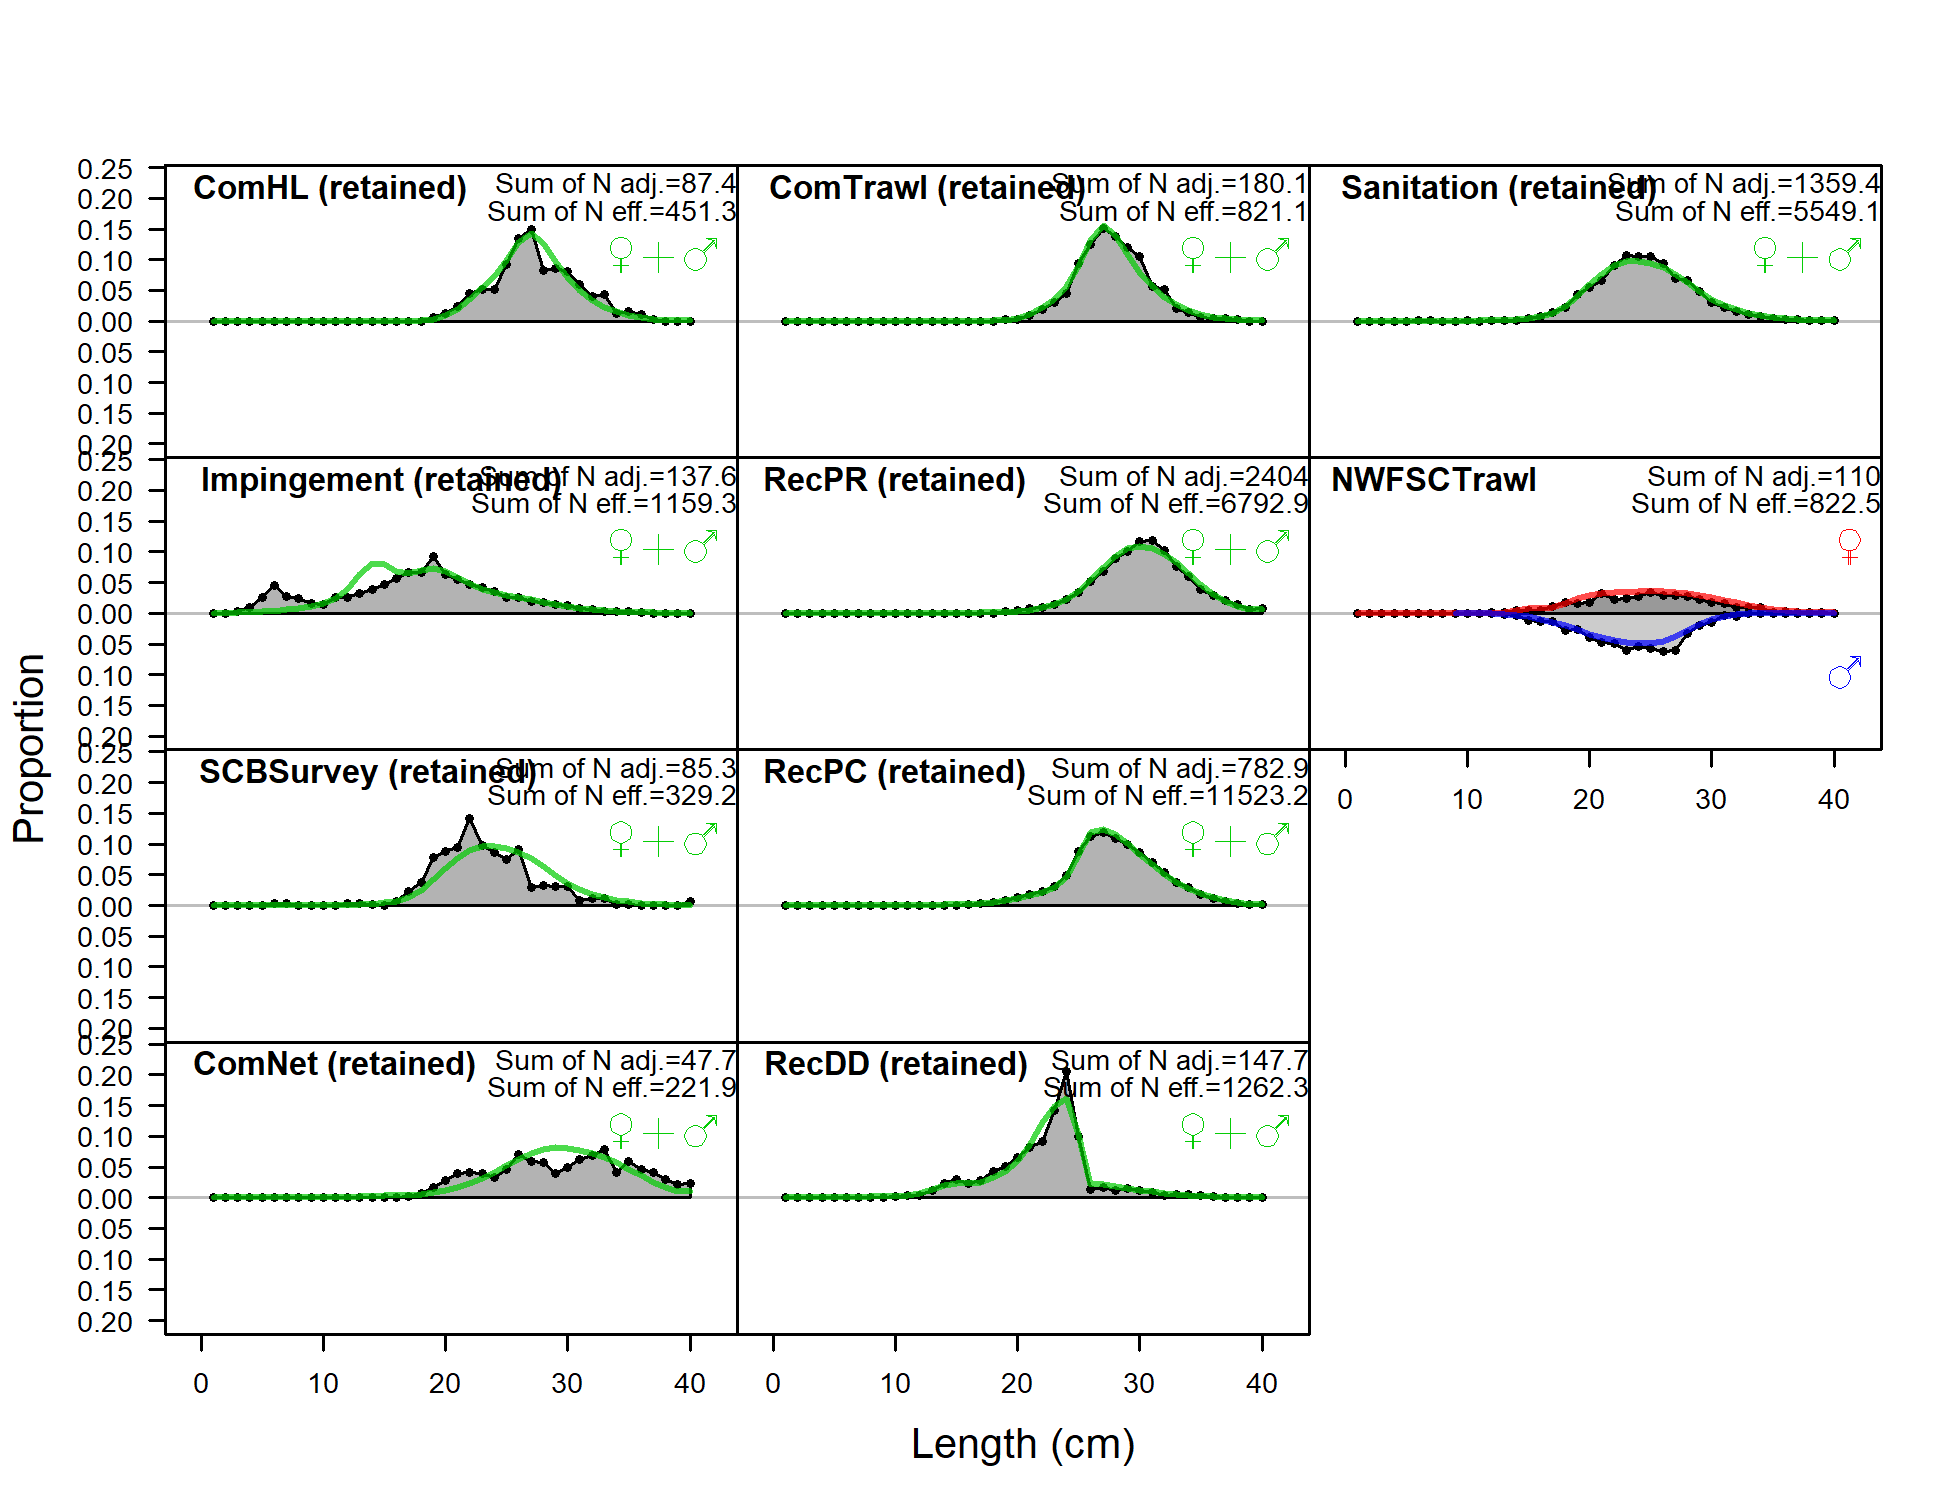
\includegraphics{r4ss/plots_mod1/comp_lenfit__aggregated_across_time.png}

\end{frame}

\begin{frame}{Commercial fishery length composition}

\begincols
 \begincol{.5\textwidth} \centering
 Commercial hook-and-line
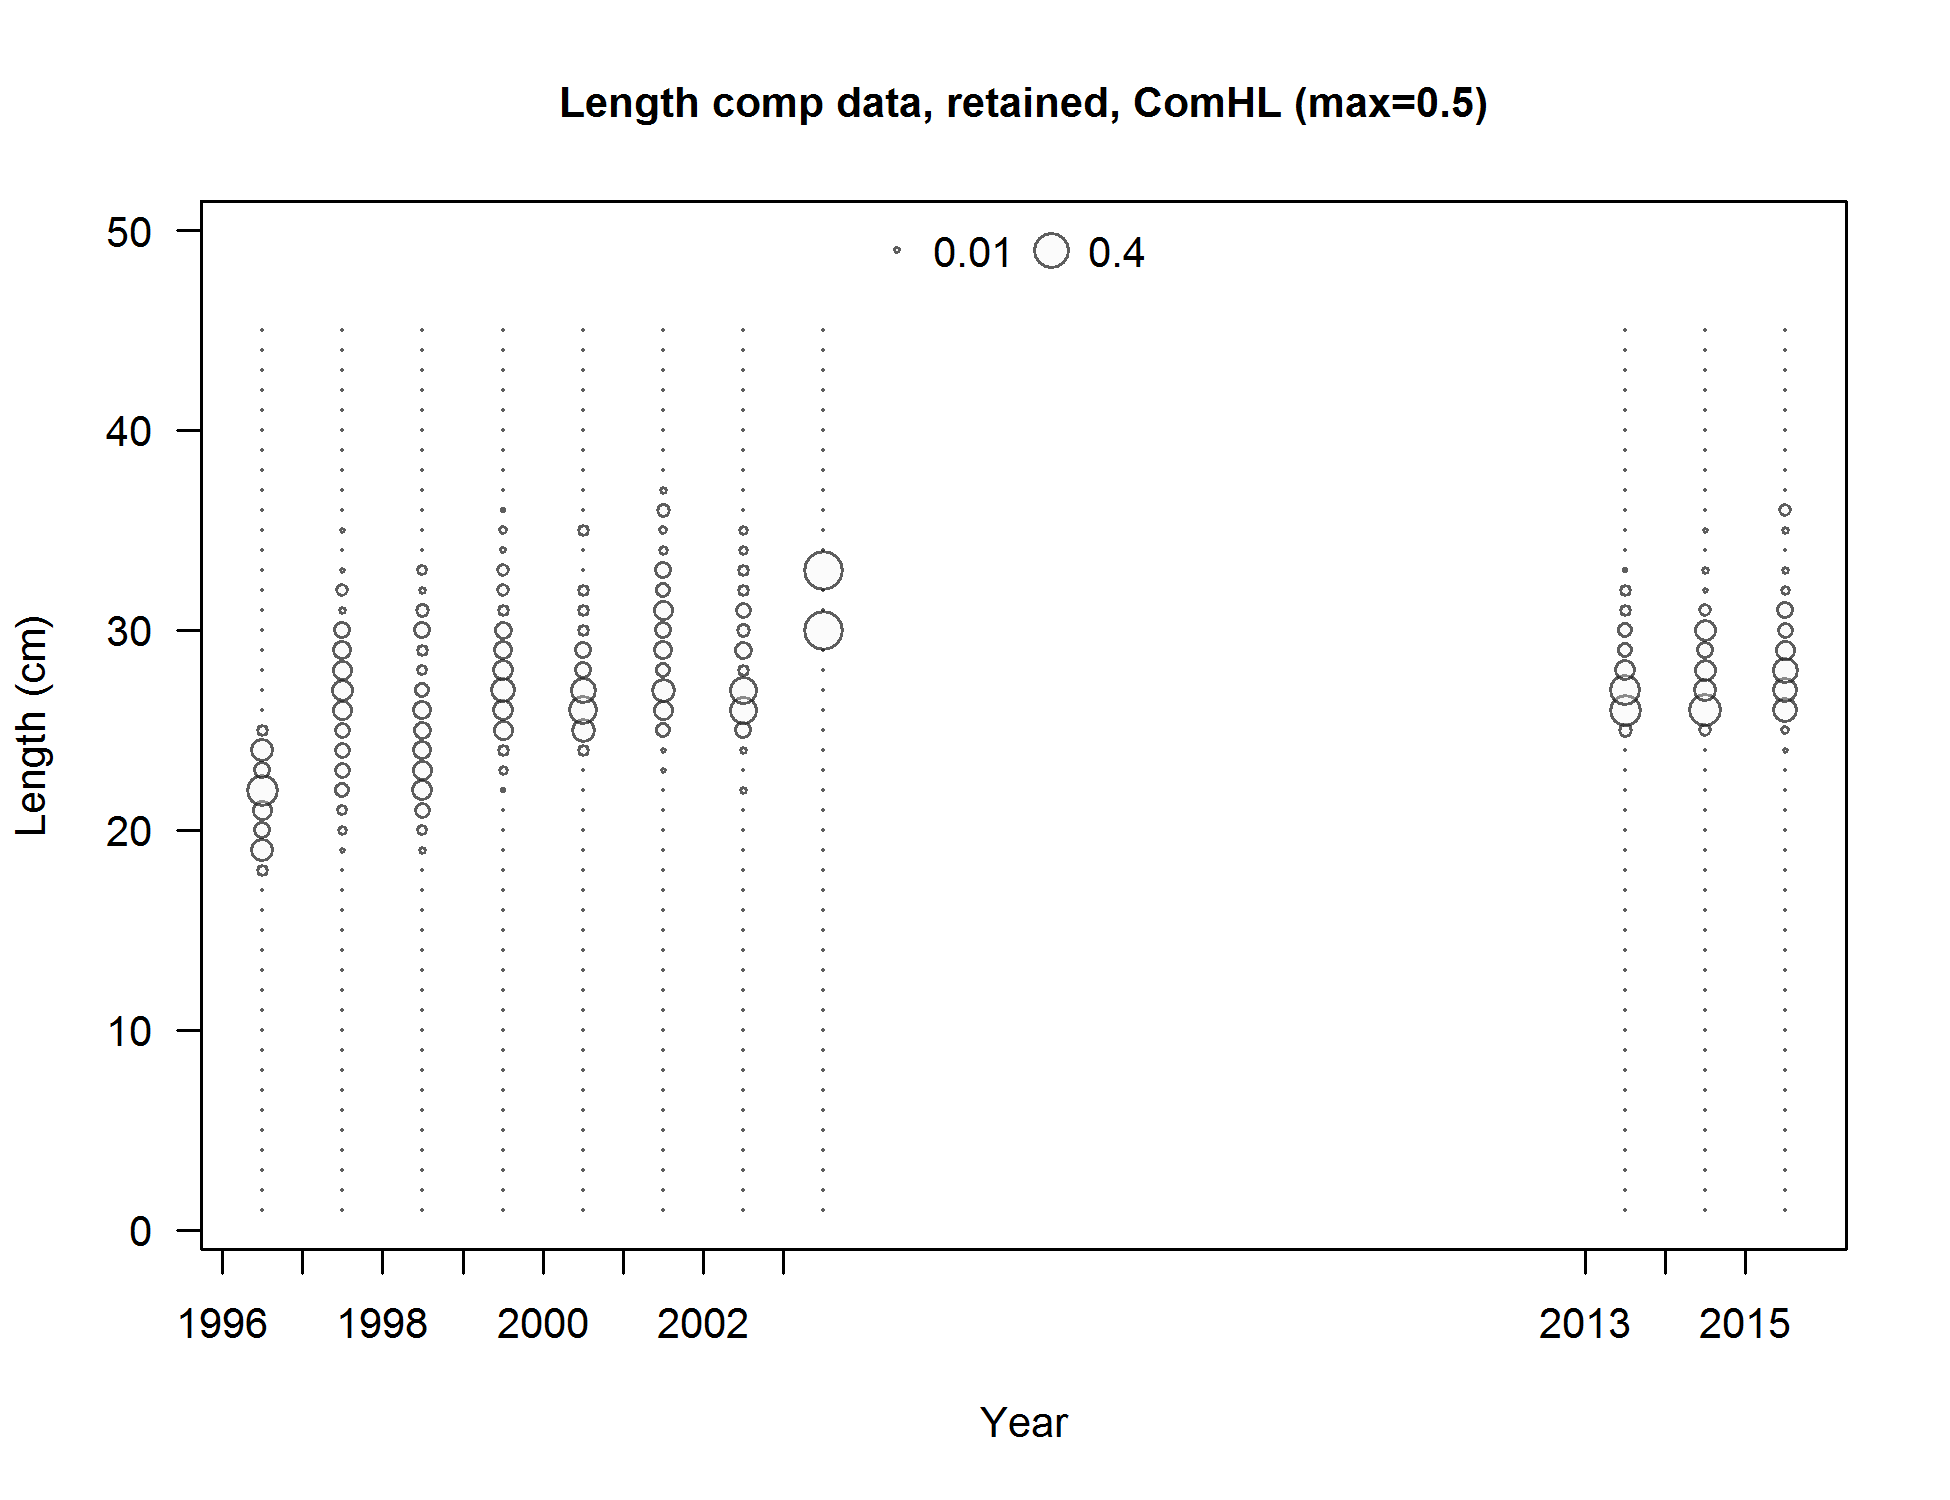
\includegraphics[height=3cm]{r4ss/plots_mod1/comp_lendat_bubflt1mkt2.png}

Commercial gillnet
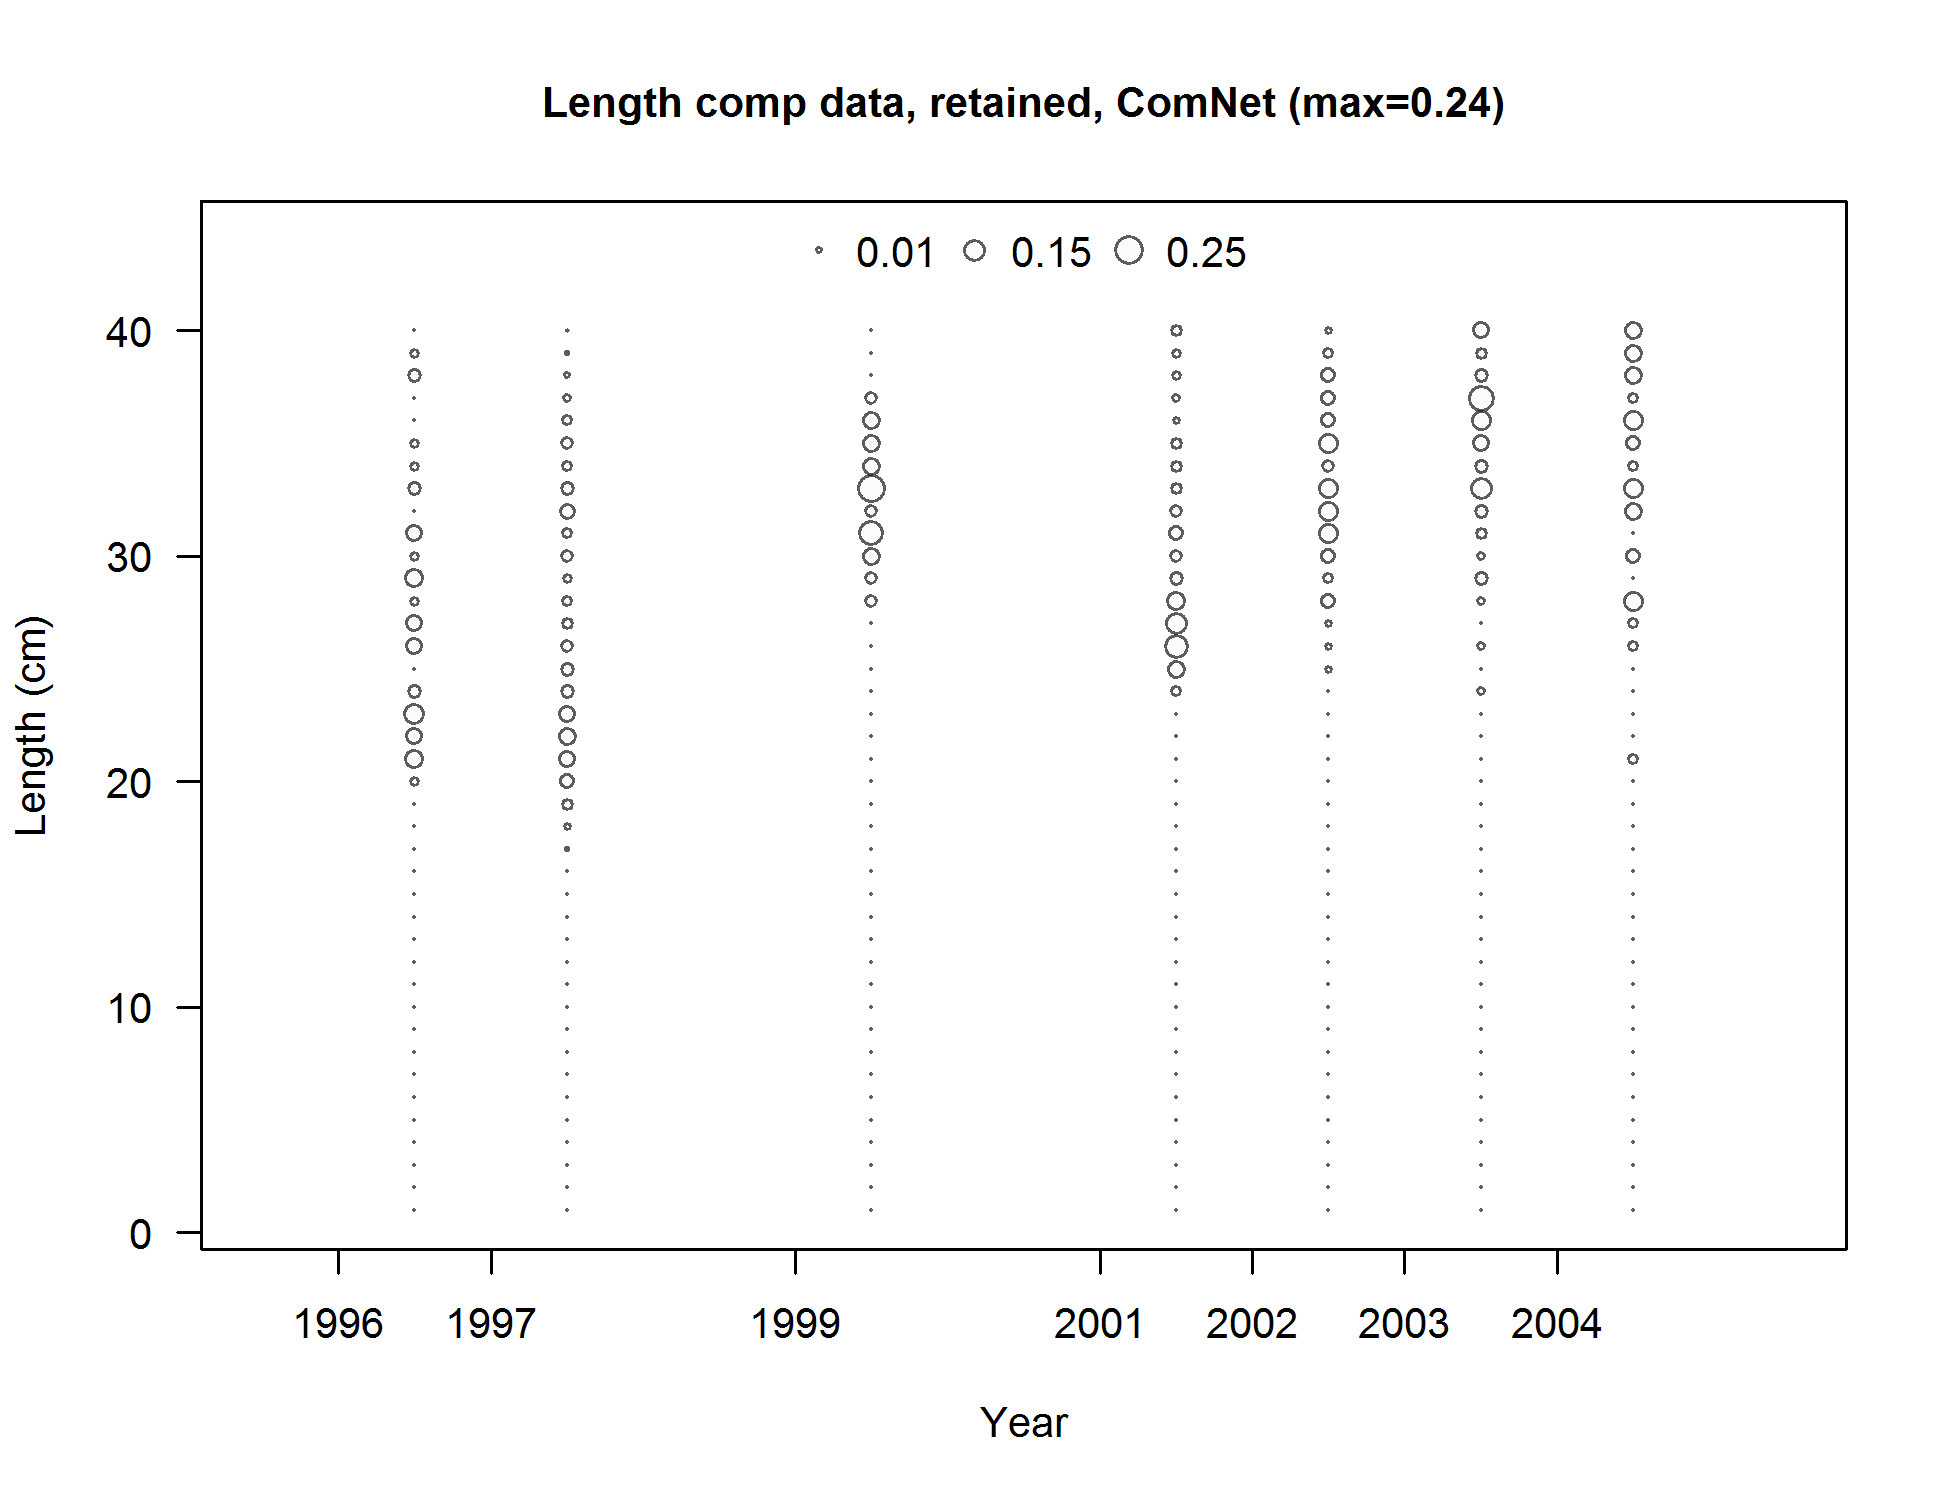
\includegraphics[height=3cm]{r4ss/plots_mod1/comp_lendat_bubflt2mkt2.png}
\endcol
 \begincol{.5\textwidth} \centering
 Commercial trawl
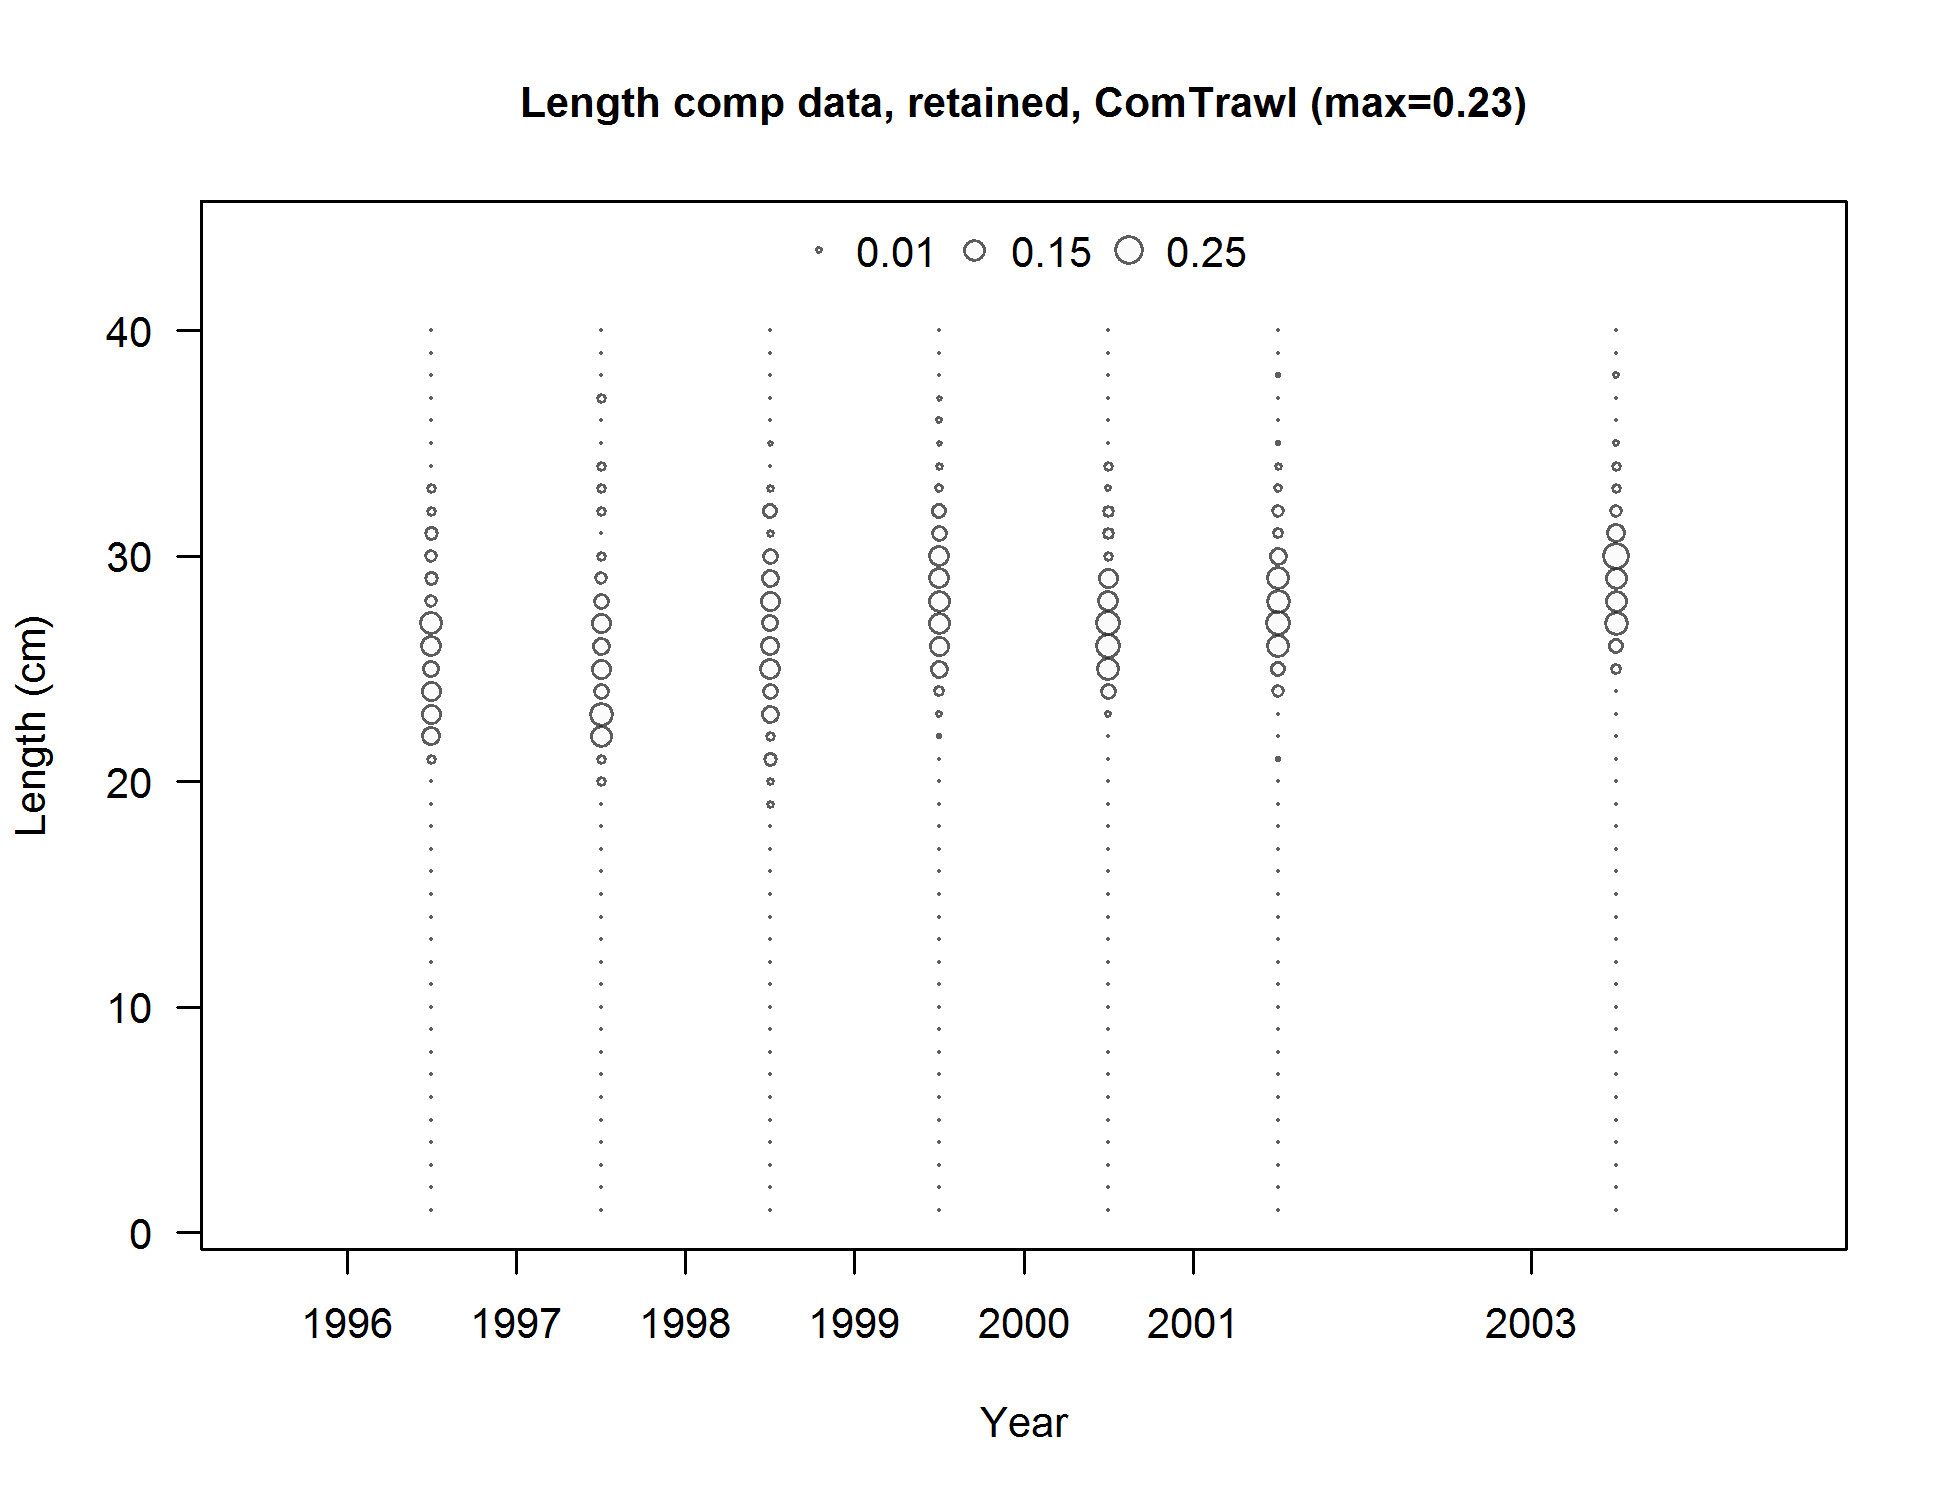
\includegraphics[height=4cm]{r4ss/plots_mod1/comp_lendat_bubflt3mkt2.png}
\endcol
\endcols

\end{frame}

\begin{frame}{Recreational fishery Length Composition}

\begincols
 \begincol{.5\textwidth} Recreational private fleet
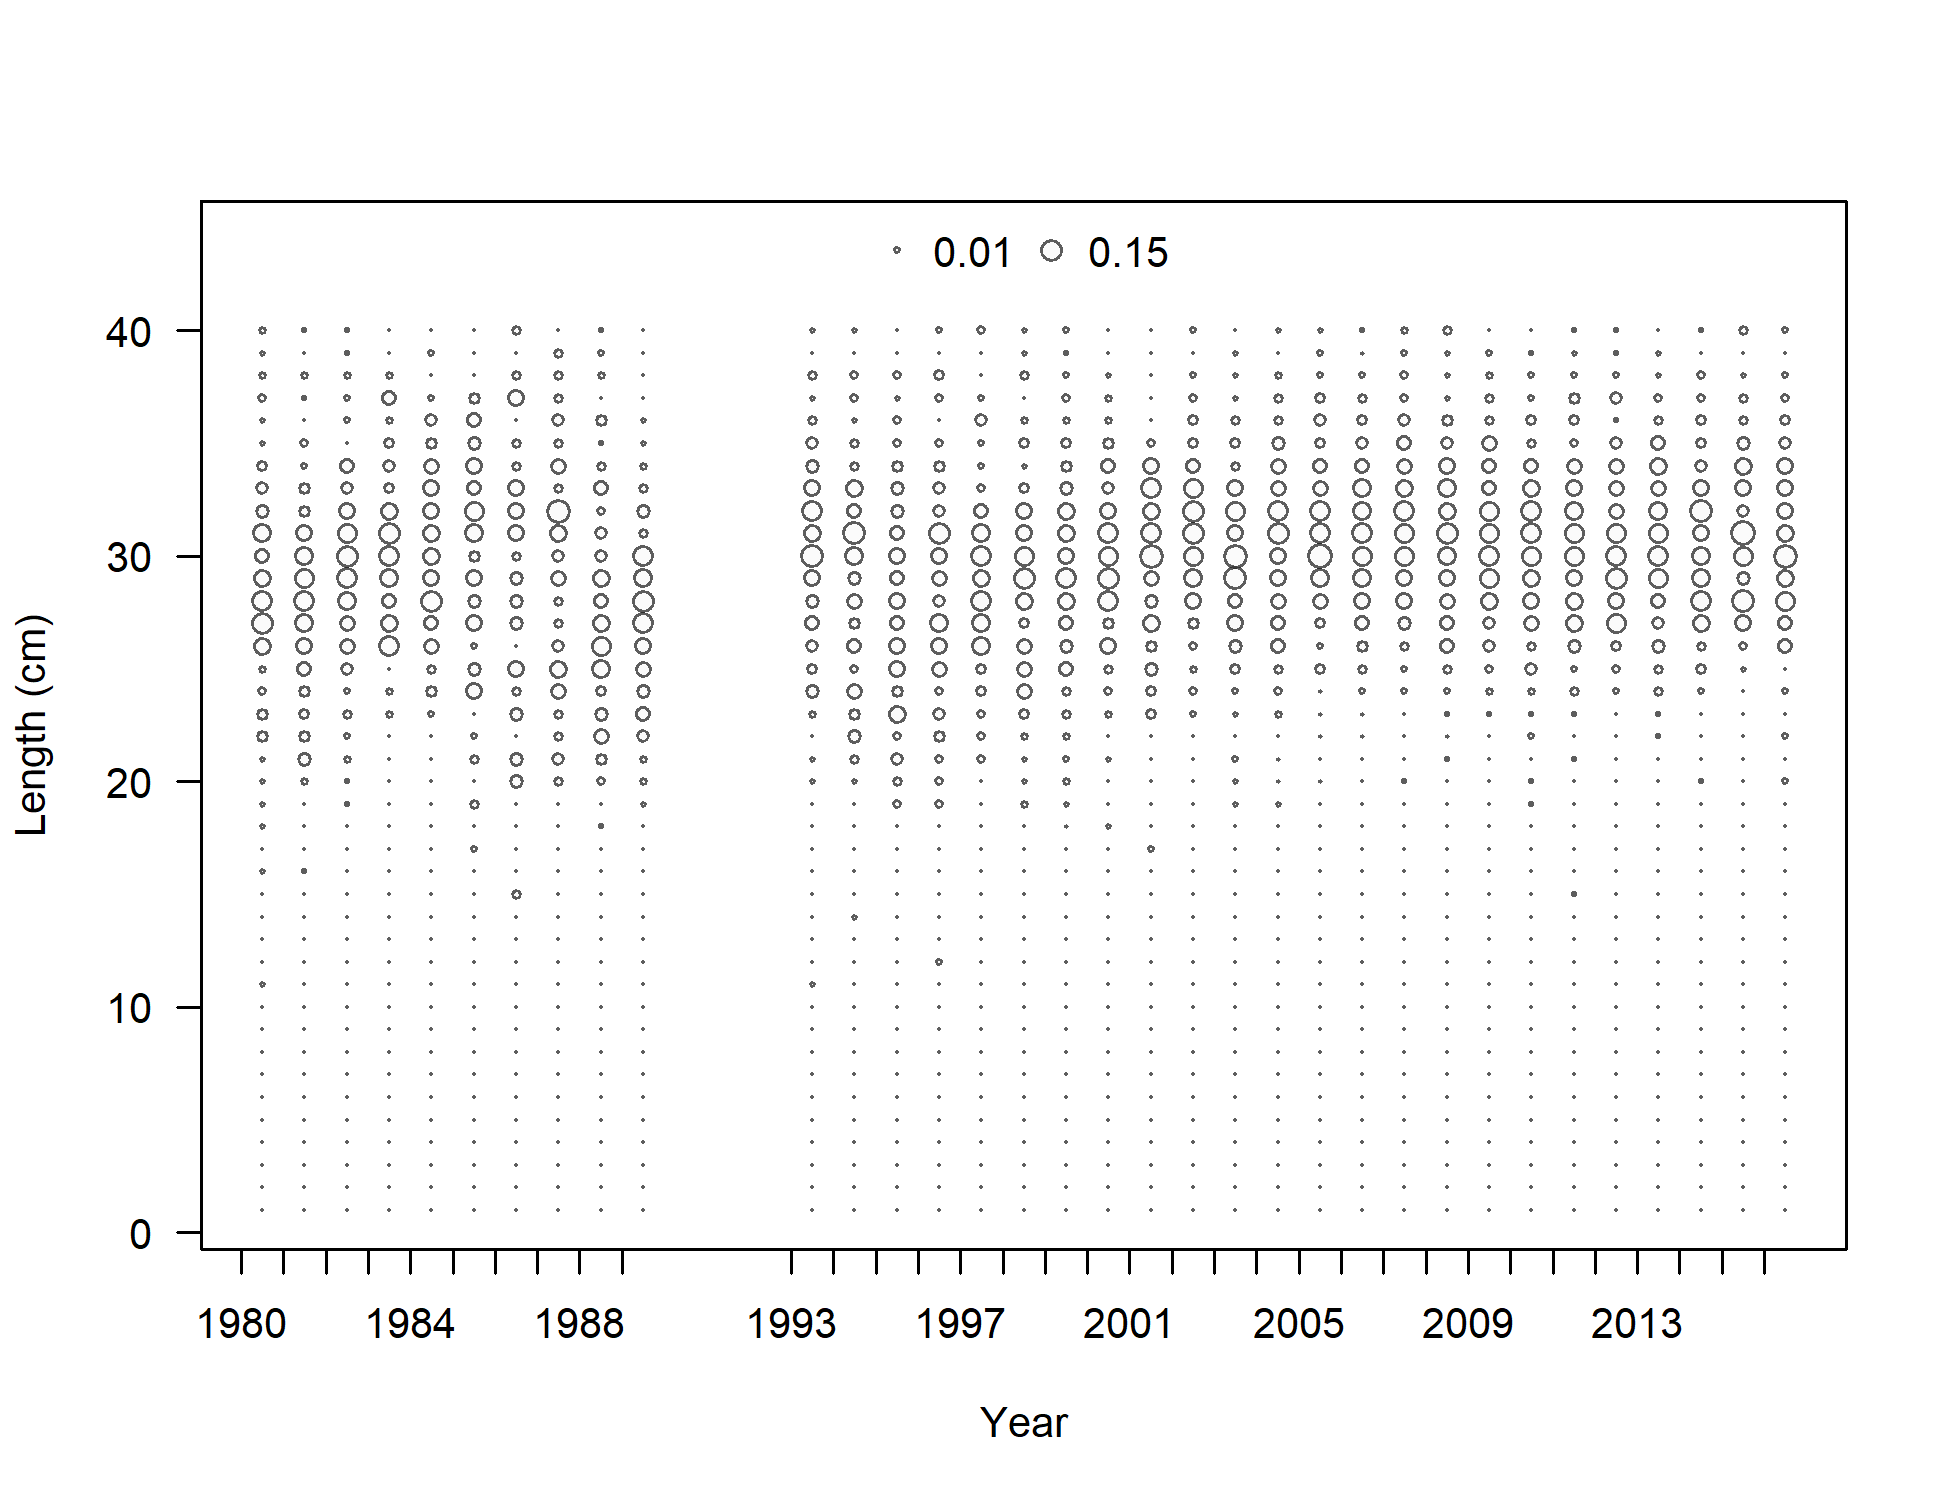
\includegraphics[height=3cm]{r4ss/plots_mod1/comp_lendat_bubflt4mkt2.png}

Recreational party/charter fleet
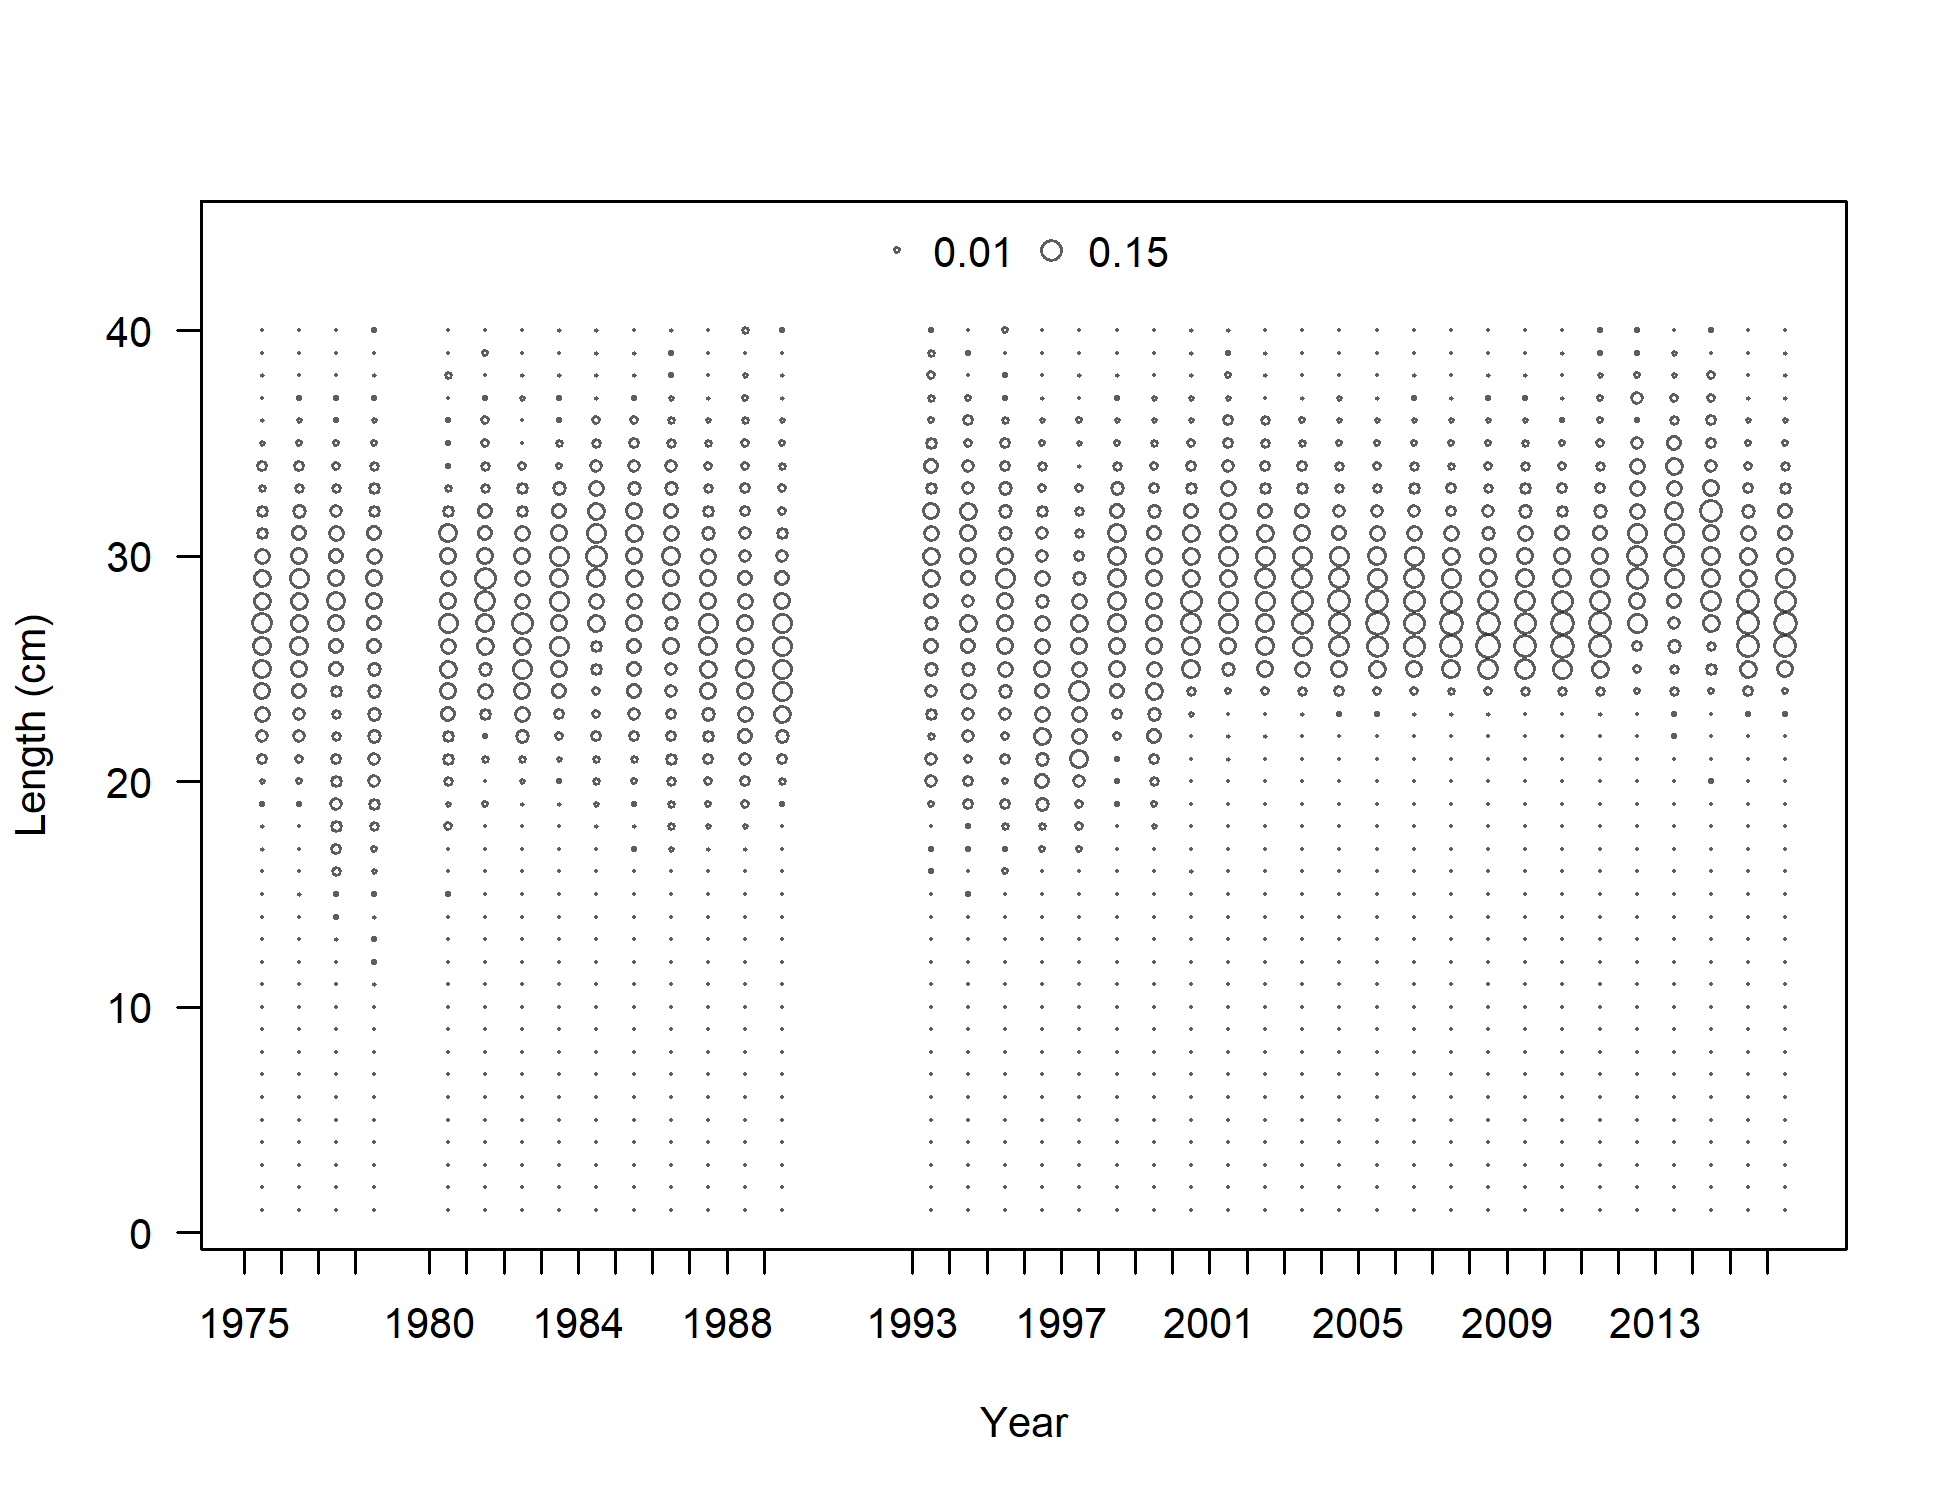
\includegraphics[height=3cm]{r4ss/plots_mod1/comp_lendat_bubflt5mkt2_page2.png}
\endcol
 \begincol{.5\textwidth} \centering

Recreational dead discards
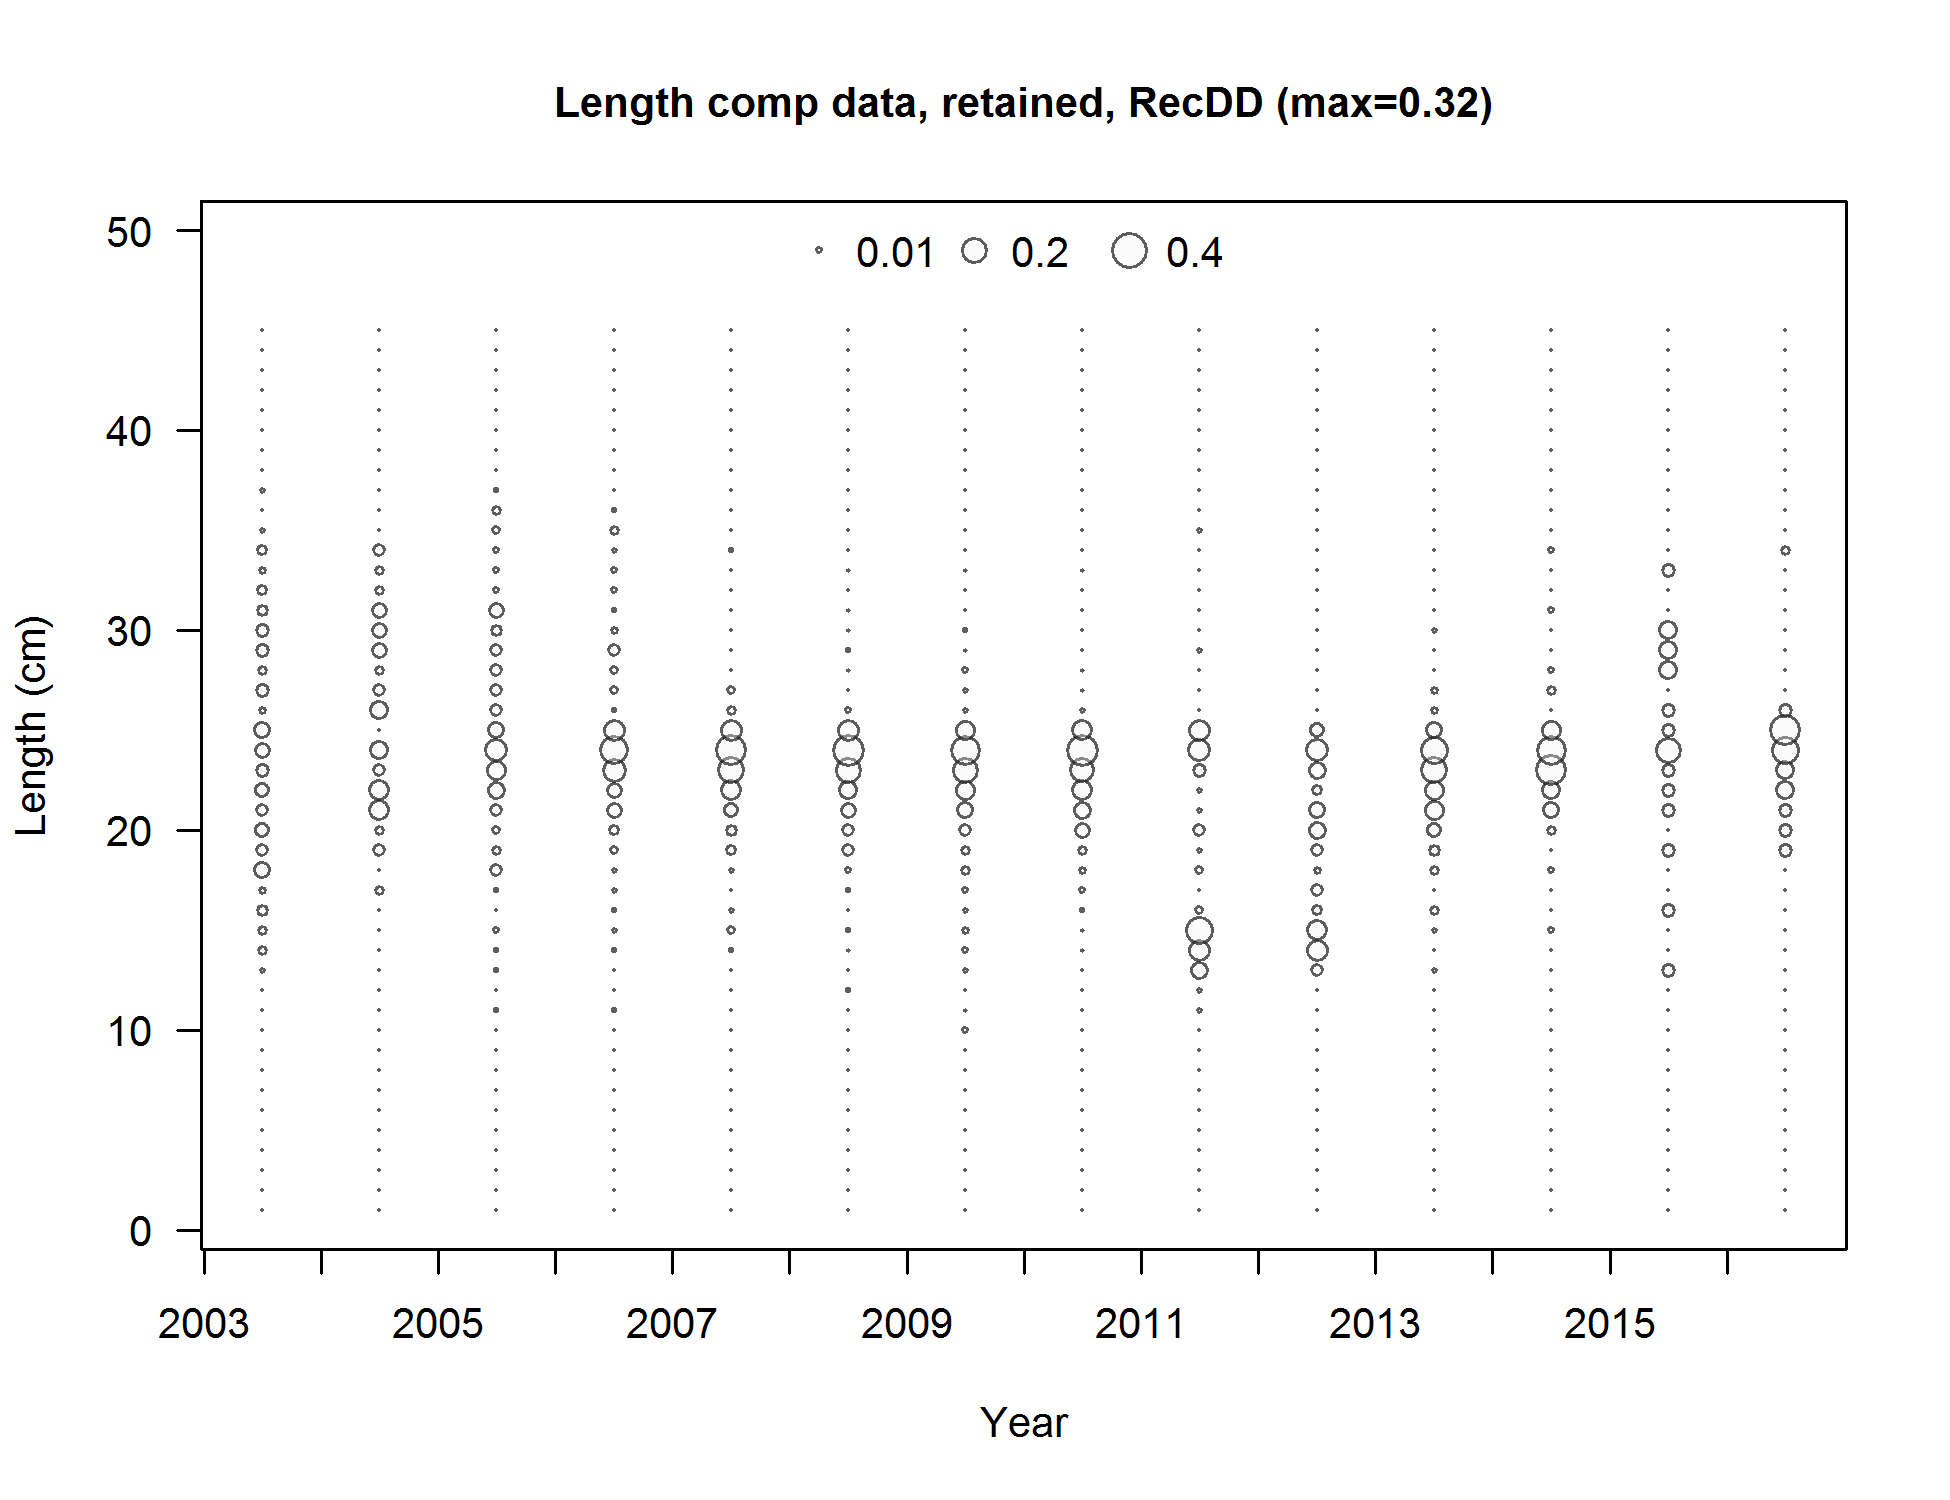
\includegraphics[height=4cm]{r4ss/plots_mod1/comp_lendat_bubflt6mkt2.png}
\endcol
\endcols

\end{frame}

\begin{frame}{Research Length Composition}

\begincols
 \begincol{.5\textwidth} POTW survey
\includegraphics[height=3cm]{r4ss/plots_mod1/comp_lendat_bubflt7mkt2_page2.png}

Gillnet survey
\includegraphics[height=3cm]{r4ss/plots_mod1/comp_lendat_bubflt9mkt2.png}
\endcol
 \begincol{.5\textwidth} Impingement survey
\includegraphics[height=3cm]{r4ss/plots_mod1/comp_lendat_bubflt10mkt2.png}

Bight trawl survey
\includegraphics[height=3cm]{r4ss/plots_mod1/comp_lendat_bubflt11mkt2.png}
\endcol
\endcols

\end{frame}

\begin{frame}{NWFSC Length and Age Composition}

Note: females in red and males in blue \begincols
 \begincol{.5\textwidth}
\includegraphics[height=.5\textheight]{r4ss/plots_mod1/comp_condAALdat_bubflt8mkt0_page1.png}
\endcol
 \begincol{.5\textwidth}
\includegraphics[height=.5\textheight]{r4ss/plots_mod1/comp_condAALdat_bubflt8mkt0_page2.png}
\endcol
\endcols

\end{frame}

\section{Biological}\label{biological}

\begin{frame}{Length data}

\begin{itemize}
\item[$\bullet$] 2005 assessment used standard length
\item[$\bullet$] Impingement, POTW, and Bight surveys measure standard length
\item[$\bullet$] 2017 assessment uses total length (conversion based on a CDFW halibut trawl study; measured both SL and TL)
\item[$\bullet$] To avoid gaps in TL length bins, TL = SL - 0.5 + U[0,1] 
\end{itemize}

\includegraphics[height=.5\textheight]{Figures/SL_to_TL_compare.png}

\end{frame}

\begin{frame}{Length data}

POTW lengths \begincols
 \begincol{.4\textwidth}
\includegraphics{Figures/Fleet7_Sanitation_lengthboxplots.png} \endcol
 \begincol{.6\textwidth}
\includegraphics{Figures/Fleet7_Sanitation_length_source.png}\\
\endcol
\endcols

\end{frame}

\begin{frame}{Length-at-Age}

\begincols
 \begincol{.4\textwidth}
\includegraphics[trim={0 0 0 2cm}, totalheight=0.65\textheight]{Figures/Age_length_bySex.png}
\endcol
 \begincol{.48\textwidth} \includegraphics{Figures/vonB_compare.png}
\endcol
\endcols

\end{frame}

\begin{frame}{Length-at-Age}

\begincols
 \begincol{.4\textwidth}
\includegraphics{Figures/NWFSCtrawl_lengthdepth.png} \endcol
\begincol{.48\textwidth}
\includegraphics{r4ss/plots_mod1/comp_lendat_bubflt8mkt0.png} \endcol
\endcols

\end{frame}

\begin{frame}{Maturity and Fecundity}

\begincols
 \begincol{.5\textwidth}

\begin{itemize}
\item[$\bullet$] Only information on maturity from Love et al. (1987)
\item[$\bullet$] Found over 50\% of females were mature by 18 cm TL, or two years of age. 
\item[$\bullet$] All fish were mature by 22 cm TL
\item[$\bullet$] No information available on fecundity of California scorpionfish
\end{itemize}

\endcol
 \begincol{.5\textwidth}
\includegraphics[height=5cm]{r4ss/plots_mod1/bio6_maturity.png} \endcol
\endcols

\end{frame}

\begin{frame}{Ageing Error}

\begincols
 \begincol{.5\textwidth}
\includegraphics[height=6cm]{Figures/otolith1.pdf} \endcol
 \begincol{.5\textwidth}

\includegraphics[height=6cm]{Figures/Fleet8_NWFSCTrawl_ageerror.png}\\
\endcol
\endcols

\end{frame}

\begin{frame}{Ageing Error}

\includegraphics{Figures/Fleet8_NWFSCTrawl_ageerror2.pdf}

\end{frame}

\begin{frame}{Weight-at-Length}

\centering
 \includegraphics{Figures/Length_weight.png}

\end{frame}

\begin{frame}{Natural Mortality}

\begin{itemize}
\item[$\bullet$] Prior based on maximum age of 21 (maximum observed age was 27, but fish older than 21 were rare in the available ages)
\item[$\bullet$] Lognormal distribution with a median of 0.25714 (Hamel/Then prior)
\item[$\bullet$] Base model fixes female natural mortality ($M$ = 0.25714)
\item[$\bullet$] Male $M$ estimated as offset from female (male $M$ = 0.207733)
\item[$\bullet$] Sensitivities explore estimating $M$
\end{itemize}

\end{frame}

\begin{frame}{Natural Mortality}

\begincols
 \begincol{.5\textwidth} Base model - fixed female \(M\), male \(M\)
estimated as offset (\(lnR_0\) = 8.16, depl. = 0.574, female \(M\) =
0.25714, male \(M\) = 0.2077)

\includegraphics[height=6cm]{r4ss/plots_mod1/ts7_Spawning_biomass_(mt)_with_95_asymptotic_intervals_intervals.png}
\endcol
 \begincol{.5\textwidth} Base model with one \(M\) estimated (\(lnR_0\)
= 8.54, depl. = 0.595, \(M\) = 0.266)

\includegraphics{Figures/SpawnB_BaseOneM.png}\\
\endcol
\endcols

\end{frame}

\begin{frame}{Steepness: Density-Dependent Recruitment Compensation}

\begin{itemize}
\item[$\bullet$] Predictive distribution for Pacific rockfish meta-analysis
\item[$\bullet$] Prior median in 2017 for steepness ($h$) = 0.718
\end{itemize}

\centering
\includegraphics[height=6cm]{Figures/h_prior.png}

\end{frame}

\section{Model}\label{model}

\begin{frame}{Model Specifications}

\begin{itemize}
\item[$\bullet$] Stock Synthesis version 3.30.05.04
\item[$\bullet$] Model starts in 1916, unfished equilibrium catch prior to that
\item[$\bullet$] Sex-specific growth and mortality with female $M$ fixed at 0.2571 (prior) and male $M$ offset is estimated at -0.2134 (male $M$ = 0.2077)
\begin{itemize}
\item[$\circ$] $M$ fixed at 0.25 for both sexes in 2005 assessment
\end{itemize}
\item[$\bullet$] Steepness fixed at 0.718 (from meta-analysis)
\begin{itemize}
\item[$\circ$] $h$ fixed at 0.7 in 2005 assessment
\end{itemize}
\item[$\bullet$] Maximum age of 21
\item[$\bullet$] One cm length bins
\item[$\bullet$] Recruitment deviations estimated
\end{itemize}

\end{frame}

\begin{frame}{Selectivity}

\begin{itemize}
\item[$\bullet$] Time blocks
\begin{itemize}
\item[$\circ$] Commercial fleet: 1916-1999 and 2000-2016 (10-in. minimum size limit as of 2000)
\item[$\circ$] Recreational fleets: 1916-2000 (few regulations), 2001-2005 (fishery closures), 2006-2016 (consistent regulations)
\end{itemize}
\item[$\bullet$] Double normal except for the impingement survey (Selectivity = 1.0 for all ages)
\item[$\bullet$] Fisheries selectivity parameters estimated for commercial hook-and-line, receational private, recreational party/charter, and recreational discard fleets
\end{itemize}

\end{frame}

\begin{frame}{Selectivity}

\begin{itemize}
\item[$\bullet$] Commercial gillnet and trawl fleets mirrored to the commercial hook-and-line fleet
\item[$\bullet$] Recreational CPFV onboard observer retained catch mirrored to the recreational party/charter fleet selectivity (same boats)
\item[$\bullet$] Survey selectivity parameters estimated for the POTW and NWFSC trawl surveys
\item[$\bullet$] The gillnet survey and Bight trawl survey mirrored to the POTW selectivity 
\end{itemize}

\centering
\includegraphics[height=4cm]{r4ss/plots_mod1/sel01_multiple_fleets_length1.png}

\end{frame}

\begin{frame}{Selectivity}

\begincols
 \begincol{.5\textwidth}
\includegraphics[height=4cm]{r4ss/plots_mod1/sel03_len_timevary_surf_flt1sex1.png}

\includegraphics[height=4cm]{r4ss/plots_mod1/sel03_len_timevary_surf_flt4sex1.png}
\endcol
 \begincol{.5\textwidth}

\includegraphics[height=4cm]{r4ss/plots_mod1/sel03_len_timevary_surf_flt5sex1.png}\\
\includegraphics[height=4cm]{r4ss/plots_mod1/sel09_len_flt6sex1.png}\\
\endcol
\endcols

\end{frame}

\begin{frame}{Gear Selectivity}

\begincols
 \begincol{.5\textwidth}
\includegraphics[height=4cm]{r4ss/plots_mod1/sel09_len_flt7sex1.png}

\endcol
 \begincol{.5\textwidth}
\includegraphics[height=4cm]{r4ss/plots_mod1/sel09_len_flt8sex1.png}
\endcol
\endcols

\end{frame}

\begin{frame}{Data Weighting}

\begin{itemize}
\item[$\bullet$] Extra SD estimated for indices
\item[$\bullet$] Francis weighting applied to length and age data
\item[$\bullet$] Conducted sensitivities to no weighting and harmonic means
\end{itemize}

\begincols
 \begincol{.5\textwidth}
\includegraphics[height=4cm]{Figures/Data_weighting_spawnb.png} \endcol
 \begincol{.5\textwidth}
\includegraphics[height=4cm]{Figures/Data_weighting_Bratio.png} \endcol
\endcols

\end{frame}

\begin{frame}{Convergence}

\begin{itemize}
\item[$\bullet$] Confirmed that the Hessian was positive definite
\item[$\bullet$] Final gradient is $<$0.0001
\item[$\bullet$] Performed 50 trials using a 'jitter' to assess the model's ability to recover similar likelihood esimates when initialized from dispersed starting points
\item[$\bullet$] The maximum difference in the likelihood from the jitter runs was 14.68 and 56\% of runs were at the minimum likelihood
\end{itemize}

\end{frame}

\begin{frame}{Pre-STAR Base Model Output (page 1)}

\begin{table}[ht]
\centering
\scalebox{0.5}{
\begin{tabular}{p{1.9in}p{.6in}p{.6in}p{.9in}p{.4in}p{.4in}p{2in}}
  \hline
Parameter & Value & Phase & Bounds & Status & SD & Prior (Exp.Val, SD) \\ 
  \hline
NatM\_p\_1\_Fem\_GP\_1 & 0.257 & -3 & (0.01, 1) &  &  & Log\_Norm (-1.3581, 0.438438) \\ 
  L\_at\_Amin\_Fem\_GP\_1 & 12.434 & 2 & (2, 30) & OK & 0.626 & None \\ 
  L\_at\_Amax\_Fem\_GP\_1 & 33.312 & 2 & (30, 50) & OK & 0.720 & None \\ 
  VonBert\_K\_Fem\_GP\_1 & 0.250 & 2 & (0.05, 0.5) & OK & 0.024 & None \\ 
  CV\_young\_Fem\_GP\_1 & 0.089 & 3 & (0.02, 0.5) & OK & 0.019 & None \\ 
  CV\_old\_Fem\_GP\_1 & 0.112 & 3 & (0.02, 0.75) & OK & 0.008 & None \\ 
  Wtlen\_1\_Fem & 0.000 & -3 & (-3, 3) &  &  & None \\ 
  Wtlen\_2\_Fem & 3.058 & -3 & (2, 4) &  &  & None \\ 
  Mat50\%\_Fem & 18.000 & -3 & (10, 30) &  &  & None \\ 
  Mat\_slope\_Fem & -1.200 & -3 & (-3, 3) &  &  & None \\ 
  Eggs/kg\_inter\_Fem & 1.000 & -3 & (-3, 3) &  &  & None \\ 
  Eggs/kg\_slope\_wt\_Fem & 0.000 & -3 & (-3, 3) &  &  & None \\ 
  NatM\_p\_1\_Mal\_GP\_1 & -0.213 & 2 & (-1, 1) & OK & 0.049 & Normal (0, 99) \\ 
  L\_at\_Amin\_Mal\_GP\_1 & 0.000 & -2 & (-3, 3) &  &  & None \\ 
  L\_at\_Amax\_Mal\_GP\_1 & -0.159 & 2 & (-3, 3) & OK & 0.026 & None \\ 
  VonBert\_K\_Mal\_GP\_1 & -0.295 & 2 & (-3, 3) & OK & 0.183 & None \\ 
  CV\_young\_Mal\_GP\_1 & 1.300 & 3 & (-3, 3) & OK & 0.218 & None \\ 
  CV\_old\_Mal\_GP\_1 & -0.452 & 3 & (-3, 3) & OK & 0.158 & None \\ 
  Wtlen\_1\_Mal & 0.000 & -5 & (0, 1) &  &  & None \\ 
  Wtlen\_2\_Mal & 2.981 & -5 & (2, 4) &  &  & None \\ 
  CohortGrowDev & 1.000 & -1 & (1, 1) &  &  & None \\ 
  FracFemale\_GP\_1 & 0.500 & -4 & (0.000001, 0.999999) &  &  & None \\ 
  SR\_LN(R0) & 8.160 & 1 & (0, 31) & OK & 0.157 & None \\ 
  SR\_BH\_steep & 0.718 & -2 & (0.21, 0.99) &  &  & Full\_Beta (0.718, 0.158) \\ 
   \hline
\end{tabular}
}
\end{table}

\end{frame}

\begin{frame}{Pre-STAR Base Model Output (page 2)}

\begin{table}[ht]
\centering
\scalebox{0.5}{
\begin{tabular}{p{1.9in}p{.6in}p{.6in}p{.9in}p{.4in}p{.4in}p{2in}}
  \hline
Parameter & Value & Phase & Bounds & Status & SD & Prior (Exp.Val, SD) \\ 
  \hline
SR\_sigmaR & 0.600 & -2 & (0, 2) &  &  & None \\ 
  SR\_regime & 0.000 & -4 & (-5, 5) &  &  & None \\ 
  SR\_autocorr & 0.000 & -3 & (0, 0.5) &  &  & None \\ 
  LnQ\_base\_RecPR(4) & -6.775 & -1 & (-15, 15) &  &  & None \\ 
  Q\_extraSD\_RecPR(4) & 0.013 & 4 & (0.0001, 1) & OK & 0.020 & None \\ 
  LnQ\_base\_RecPC(5) & -11.223 & -1 & (-15, 15) &  &  & None \\ 
  Q\_extraSD\_RecPC(5) & 0.267 & 4 & (0.0001, 1) & OK & 0.047 & None \\ 
  LnQ\_base\_RecDD(6) & -10.894 & -1 & (-15, 15) &  &  & None \\ 
  Q\_extraSD\_RecDD(6) & 0.078 & 4 & (0.0001, 1) & OK & 0.044 & None \\ 
  LnQ\_base\_Sanitation(7) & -10.544 & -1 & (-15, 15) &  &  & None \\ 
  Q\_extraSD\_Sanitation(7) & 0.225 & 4 & (0.0001, 1) & OK & 0.047 & None \\ 
  LnQ\_base\_NWFSCTrawl(8) & -1.023 & -1 & (-15, 15) &  &  & None \\ 
  Q\_extraSD\_NWFSCTrawl(8) & 0.250 & 4 & (0.0001, 1) & OK & 0.145 & None \\ 
  LnQ\_base\_GillnetSurvey(9) & -12.050 & -1 & (-15, 15) &  &  & None \\ 
  Q\_extraSD\_GillnetSurvey(9) & 0.122 & 4 & (0.0001, 1) & OK & 0.070 & None \\ 
  LnQ\_base\_SCBSurvey(11) & -11.052 & -1 & (-15, 15) &  &  & None \\ 
  Q\_extraSD\_SCBSurvey(11) & 0.166 & 4 & (0.0001, 1) & OK & 0.142 & None \\ 
  LnQ\_base\_RecPCOBR(12) & -10.171 & -1 & (-15, 15) &  &  & None \\ 
  Q\_extraSD\_RecPCOBR(12) & 0.140 & 4 & (0.0001, 1) & OK & 0.046 & None \\ 
  SizeSel\_P1\_ComHL(1) & 25.963 & 5 & (13, 44) & OK & 2.868 & None \\ 
  SizeSel\_P2\_ComHL(1) & 15.000 & -3 & (-10, 16) &  &  & None \\ 
  SizeSel\_P3\_ComHL(1) & 2.761 & 5 & (-1, 10) & OK & 0.954 & None \\ 
  SizeSel\_P4\_ComHL(1) & 15.000 & -3 & (-1, 16) &  &  & None \\ 
  SizeSel\_P5\_ComHL(1) & -15.902 & 5 & (-25, -1) & OK & 121.578 & None \\ 
  SizeSel\_P6\_ComHL(1) & 10.000 & -3 & (-5, 11) &  &  & None \\ 
  SizeSel\_P1\_ComNet(2) & 1.000 & -2 & (1, 45) &  &  & None \\ 
   \hline
\end{tabular}
}
\end{table}

\end{frame}

\begin{frame}{Pre-STAR Base Model Output (page 3)}

\begin{table}[ht]
\centering
\scalebox{0.5}{
\begin{tabular}{p{1.9in}p{.6in}p{.6in}p{.9in}p{.4in}p{.4in}p{2.1in}}
  \hline
Parameter & Value & Phase & Bounds & Status & SD & Prior (Exp.Val, SD) \\ 
  \hline
SizeSel\_P2\_ComNet(2) & 45.000 & -3 & (1, 45) &  &  & None \\ 
  SizeSel\_P1\_ComTrawl(3) & 1.000 & -2 & (1, 45) &  &  & None \\ 
  SizeSel\_P2\_ComTrawl(3) & 45.000 & -3 & (1, 45) &  &  & None \\ 
  SizeSel\_P1\_RecPR(4) & 41.212 & 5 & (13, 44) & OK & 2.054 & None \\ 
  SizeSel\_P2\_RecPR(4) & 15.000 & -3 & (-10, 16) &  &  & None \\ 
  SizeSel\_P3\_RecPR(4) & 4.493 & 5 & (-1, 10) & OK & 0.163 & None \\ 
  SizeSel\_P4\_RecPR(4) & 15.000 & -3 & (-1, 16) &  &  & None \\ 
  SizeSel\_P5\_RecPR(4) & -8.340 & 5 & (-25, -1) & OK & 0.784 & None \\ 
  SizeSel\_P6\_RecPR(4) & 10.000 & -3 & (-5, 11) &  &  & None \\ 
  SizeSel\_P1\_RecPC(5) & 36.624 & 5 & (13, 44) & OK & 1.358 & None \\ 
  SizeSel\_P2\_RecPC(5) & 15.000 & -3 & (-10, 16) &  &  & None \\ 
  SizeSel\_P3\_RecPC(5) & 4.473 & 5 & (-1, 10) & OK & 0.158 & None \\ 
  SizeSel\_P4\_RecPC(5) & 15.000 & -3 & (-1, 16) &  &  & None \\ 
  SizeSel\_P5\_RecPC(5) & -8.344 & 5 & (-25, -1) & OK & 1.872 & None \\ 
  SizeSel\_P6\_RecPC(5) & 10.000 & -3 & (-5, 11) &  &  & None \\ 
  SizeSel\_P1\_RecDD(6) & 24.530 & 5 & (13, 44) & OK & 0.074 & None \\ 
  SizeSel\_P2\_RecDD(6) & -11.238 & 4 & (-15, 16) & OK & 57.708 & None \\ 
  SizeSel\_P3\_RecDD(6) & 2.727 & 4 & (-1, 10) & OK & 0.518 & None \\ 
  SizeSel\_P4\_RecDD(6) & -9.302 & 4 & (-20, 5) & OK & 65.524 & None \\ 
  SizeSel\_P5\_RecDD(6) & -2.156 & 5 & (-25, 3) & OK & 0.472 & None \\ 
  SizeSel\_P6\_RecDD(6) & -1.709 & 4 & (-5, 11) & OK & 0.457 & None \\ 
  SizeSel\_P1\_Sanitation(7) & 24.627 & 4 & (13, 44) & OK & 0.580 & None \\ 
  SizeSel\_P2\_Sanitation(7) & 15.000 & -3 & (-10, 16) &  &  & None \\ 
  SizeSel\_P3\_Sanitation(7) & 3.388 & 4 & (-1, 10) & OK & 0.140 & None \\ 
  SizeSel\_P4\_Sanitation(7) & 15.000 & -3 & (-1, 16) &  &  & None \\ 
   \hline
\end{tabular}
}
\end{table}

\end{frame}

\begin{frame}{Pre-STAR Base Model Output (page 4)}

\begin{table}[ht]
\centering
\scalebox{0.5}{
\begin{tabular}{p{2.5in}p{.6in}p{.6in}p{.9in}p{.4in}p{.4in}p{.4in}}
  \hline
Parameter & Value & Phase & Bounds & Status & SD & Prior (Exp.Val, SD) \\ 
  \hline
SizeSel\_P4\_Sanitation(7) & 15.000 & -3 & (-1, 16) &  &  & None \\ 
  SizeSel\_P5\_Sanitation(7) & -4.618 & 4 & (-25, 5) & OK & 0.633 & None \\ 
  SizeSel\_P6\_Sanitation(7) & 10.000 & -3 & (-5, 11) &  &  & None \\ 
  SizeSel\_P1\_NWFSCTrawl(8) & 24.306 & 4 & (13, 44) & OK & 2.258 & None \\ 
  SizeSel\_P2\_NWFSCTrawl(8) & 15.000 & -3 & (-10, 16) &  &  & None \\ 
  SizeSel\_P3\_NWFSCTrawl(8) & 3.652 & 4 & (-1, 10) & OK & 0.558 & None \\ 
  SizeSel\_P4\_NWFSCTrawl(8) & 15.000 & -3 & (-1, 16) &  &  & None \\ 
  SizeSel\_P5\_NWFSCTrawl(8) & -12.844 & 4 & (-25, 5) & OK & 166.385 & None \\ 
  SizeSel\_P6\_NWFSCTrawl(8) & 10.000 & -3 & (-5, 11) &  &  & None \\ 
  SizeSel\_P1\_GillnetSurvey(9) & 1.000 & -2 & (1, 45) &  &  & None \\ 
  SizeSel\_P2\_GillnetSurvey(9) & 45.000 & -3 & (1, 45) &  &  & None \\ 
  SizeSel\_P1\_SCBSurvey(11) & 1.000 & -2 & (1, 45) &  &  & None \\ 
  SizeSel\_P2\_SCBSurvey(11) & 45.000 & -3 & (1, 45) &  &  & None \\ 
  SizeSel\_P1\_RecPCOBR(12) & 1.000 & -2 & (1, 45) &  &  & None \\ 
  SizeSel\_P2\_RecPCOBR(12) & 45.000 & -3 & (1, 45) &  &  & None \\ 
  SizeSel\_P1\_ComHL(1)\_BLK1repl\_1999 & 28.442 & 6 & (13, 44) & OK & 0.489 & None \\ 
  SizeSel\_P3\_ComHL(1)\_BLK1repl\_1999 & 2.007 & 6 & (-1, 10) & OK & 0.251 & None \\ 
  SizeSel\_P1\_RecPR(4)\_BLK2repl\_2000 & 36.584 & 6 & (13, 44) & OK & 1.031 & None \\ 
  SizeSel\_P1\_RecPR(4)\_BLK2repl\_2006 & 35.815 & 6 & (13, 44) & OK & 0.652 & None \\ 
  SizeSel\_P3\_RecPR(4)\_BLK2repl\_2000 & 3.602 & 6 & (-1, 10) & OK & 0.165 & None \\ 
  SizeSel\_P3\_RecPR(4)\_BLK2repl\_2006 & 3.463 & 6 & (-1, 10) & OK & 0.110 & None \\ 
  SizeSel\_P1\_RecPC(5)\_BLK2repl\_2000 & 31.799 & 6 & (13, 44) & OK & 1.370 & None \\ 
  SizeSel\_P1\_RecPC(5)\_BLK2repl\_2006 & 26.886 & 6 & (13, 44) & OK & 0.464 & None \\ 
  SizeSel\_P3\_RecPC(5)\_BLK2repl\_2000 & 3.041 & 6 & (-1, 10) & OK & 0.417 & None \\ 
  SizeSel\_P3\_RecPC(5)\_BLK2repl\_2006 & 1.066 & 6 & (-1, 10) & OK & 0.412 & None \\ 
   &  &  &  &  &  &  \\ 
   \hline
\end{tabular}
}
\end{table}

\end{frame}

\begin{frame}{Pre-STAR Base Model Output}

\begin{table}[ht]
\centering
\scalebox{0.8}{
\begin{tabular}{lp{1in}p{1.2in}p{1in}p{1.2in}}
  \hline
Year & Spawning biomass (mt) & \~{} 95\% confidence interval & Estimated depletion & \~{} 95\% confidence interval \\ 
  \hline
2008 & 963.57 & (555.81-1371.32) & 0.70 & (0.572-0.837) \\ 
  2009 & 927.07 & (539.76-1314.38) & 0.68 & (0.554-0.802) \\ 
  2010 & 878.16 & (513.26-1243.07) & 0.64 & (0.526-0.758) \\ 
  2011 & 841.15 & (494.98-1187.31) & 0.61 & (0.508-0.722) \\ 
  2012 & 814.87 & (483.41-1146.34) & 0.60 & (0.495-0.696) \\ 
  2013 & 765.85 & (451.39-1080.3) & 0.56 & (0.465-0.655) \\ 
  2014 & 693.82 & (401.18-986.46) & 0.51 & (0.417-0.598) \\ 
  2015 & 644.49 & (362.67-926.31) & 0.47 & (0.382-0.561) \\ 
  2016 & 681.67 & (382.78-980.56) & 0.50 & (0.399-0.597) \\ 
  2017 & 785.33 & (439.85-1130.8) & 0.57 & (0.455-0.694) \\ 
   \hline
\end{tabular}
}
\end{table}

\end{frame}

\begin{frame}{Pre-STAR Base Model Output}

\begin{table}[ht]
\centering
\scalebox{0.7}{
\begin{tabular}{p{.8in}p{.8in}p{.8in}p{.8in}p{.8in}p{.8in}}
  \hline
Year & OFL & ABC & ACL & ACT & Total Catch \\ 
  \hline
\textbf{2007} & 219 &  & 175 &  & 139.583 \\ 
  \textbf{2008} & 219 &  & 175 &  & 103.887 \\ 
  \textbf{2009} & 175 &  & 175 &  & 113.318 \\ 
  \textbf{2010} & 155 &  & 155 &  & 105.968 \\ 
  \textbf{2011} & 141 & 135 & 135 &  & 105.215 \\ 
  \textbf{2012} & 132 & 126 & 126 &  & 120.008 \\ 
  \textbf{2013} & 126 & 120 & 120 &  & 115.142 \\ 
  \textbf{2014} & 122 & 117 & 117 &  & 123.822 \\ 
  \textbf{2015} & 119 & 114 & 114 &  & 83.8908 \\ 
  \textbf{2016} & 117 & 111 & 111 &  & 74.1613 \\ 
  \textbf{2017} & 289 & 264 & 150 & 110 & - \\ 
  \textbf{2018} & 278 & 254 & 150 & 110 & - \\ 
   \hline
\end{tabular}
}
\end{table}

\end{frame}

\begin{frame}{Pre-STAR Base Model Output}

Switch to browser for r4SS output

\end{frame}

\section{Uncertainty}\label{uncertainty}

\begin{frame}{Retrospective Analysis}

Retro1 = Remove one year; Retro2 = Remove last two years; etc.
\begincols
 \begincol{.5\textwidth}
\includegraphics[height=5cm]{Figures/retro_recdev.png} \endcol
 \begincol{.5\textwidth}
\includegraphics[height=5cm]{Figures/retro_spawnb.png} \endcol
\endcols

\end{frame}

\begin{frame}{Likelihood Profiles - Natural Mortality}

\begincols
 \begincol{.5\textwidth}
\includegraphics[height=5cm]{Figures/profile_m_depl.png} \endcol
 \begincol{.5\textwidth}
\includegraphics[height=5cm]{Figures/profile_m_like.png}\\
\endcol
\endcols

\end{frame}

\begin{frame}{Likelihood Profiles - Steepness}

\begincols
 \begincol{.5\textwidth}
\includegraphics[height=5cm]{Figures/profile_h_depl.png} \endcol
 \begincol{.5\textwidth}
\includegraphics[height=5cm]{Figures/profile_h_like.png}\\
\endcol
\endcols

\end{frame}

\begin{frame}{Likelihood Profiles - \(lnR_0\)}

\begincols
 \begincol{.5\textwidth}
\includegraphics[height=5cm]{Figures/profile_R0_depl.png} \endcol
 \begincol{.5\textwidth}
\includegraphics[height=5cm]{Figures/profile_R0_like.png}\\
\endcol
\endcols

\end{frame}

\begin{frame}{Sensitivities}

Sensitivities to Likelihood Components and Model Specification
\begincols
 \begincol{.5\textwidth} \includegraphics{Figures/Sensitivity_All.pdf}
\endcol
 \begincol{.5\textwidth}

\begin{itemize}
\item Remove fleets, only one index, or length composition only
\item Sensitivity relative to the base model
\item Boxes are the 95\% CI from the base model
\item Metrics
\begin{itemize}
\item $SB_0$ Population scale
\item $SB_{2017}$ Population scale
\item $SB_{2017}/SB_{0}$ Depletion/Population status
\item $MSY_{SPR50\%}$ Yield/Productivity/scale
\end{itemize}
\end{itemize}

\endcol
\endcols

\end{frame}

\begin{frame}{Sensitivities - \(SB_0\)}

\includegraphics{Figures/Sensitivity_SB0.pdf}

\end{frame}

\begin{frame}{Sensitivities - \(SB_{2017}\)}

\includegraphics{Figures/Sensitivity_SB2017.pdf}

\end{frame}

\begin{frame}{Sensitivities - Depletion}

\includegraphics{Figures/Sensitivity_depl.pdf}

\end{frame}

\begin{frame}{Sensitivities - Yield at \(SPR_{50\%}\)}

\includegraphics{Figures/Sensitivity_Yield.pdf}

\end{frame}

\begin{frame}{Sensitivities - All}

\includegraphics{Figures/Sensitivity_Yield.pdf}

\end{frame}

\begin{frame}{Sensitivities}

\begincols
 \begincol{.5\textwidth}
\includegraphics[height=5cm]{Figures/sensitivity_spawnbio.png} \endcol
 \begincol{.5\textwidth}
\includegraphics[height=5cm]{Figures/sensitivity1_spawnbio.png}\\
\endcol
\endcols

\end{frame}

\begin{frame}{Sensitivities}

\includegraphics[height=5cm]{Figures/sensitivity2_spawnbio.png}

\end{frame}

\section{Appendix}\label{appendix}

\begin{frame}{Length Composition Fits}\includegraphics{./r4ss/plots_mod1/comp_lenfit_flt1mkt2.png}\end{frame}

\begin{frame}{Length Composition Fits}\includegraphics{./r4ss/plots_mod1/comp_lenfit_flt2mkt2.png}\end{frame}

\begin{frame}{Length Composition Fits}\includegraphics{./r4ss/plots_mod1/comp_lenfit_flt3mkt2.png}\end{frame}

\begin{frame}{Length Composition Fits}\includegraphics{./r4ss/plots_mod1/comp_lenfit_flt4mkt2.png}\end{frame}

\begin{frame}{Length Composition Fits}\includegraphics{./r4ss/plots_mod1/comp_lenfit_flt5mkt2_page1.png}\end{frame}

\begin{frame}{Length Composition Fits}\includegraphics{./r4ss/plots_mod1/comp_lenfit_flt5mkt2_page2.png}\end{frame}

\begin{frame}{Length Composition Fits}\includegraphics{./r4ss/plots_mod1/comp_lenfit_flt6mkt2.png}\end{frame}

\begin{frame}{Length Composition Fits}\includegraphics{./r4ss/plots_mod1/comp_lenfit_flt7mkt2_page1.png}\end{frame}

\begin{frame}{Length Composition Fits}\includegraphics{./r4ss/plots_mod1/comp_lenfit_flt7mkt2_page2.png}\end{frame}

\begin{frame}{Length Composition Fits}\includegraphics{./r4ss/plots_mod1/comp_lenfit_flt8mkt0.png}\end{frame}

\begin{frame}{Length Composition Fits}\includegraphics{./r4ss/plots_mod1/comp_lenfit_flt9mkt2.png}\end{frame}

\begin{frame}{Length Composition Fits}\includegraphics{./r4ss/plots_mod1/comp_lenfit_flt10mkt2.png}\end{frame}

\begin{frame}{Length Composition Fits}\includegraphics{./r4ss/plots_mod1/comp_lenfit_flt11mkt2.png}\end{frame}

\begin{frame}{Hull Method (Onboard observer index)}

\includegraphics{Figures/hull_method.png}

\end{frame}

\begin{frame}{VAST Diagnostics}

\begincols
 \begincol{.5\textwidth}

\includegraphics{Figures/Fleet8_encounter_pearson.png}

\endcol
 \begincol{.5\textwidth}

\includegraphics{Figures/Fleet8_catchrate_pearson.png}\\
\endcol
\endcols

\end{frame}

\end{document}
